\documentclass[a4paper, 12pt]{article}
\title{Adogption}
\date{2024-05-10}
\author{Laura Vega Palacios}
\renewcommand{\contentsname}{Tabla de contenidos}
\renewcommand{\listtablename}{Tabla de contenidos}
\renewcommand{\listfigurename}{Abbildungsverzeichnis}

% Paquetes
\usepackage{subcaption}
\usepackage[table]{xcolor}% http://ctan.org/pkg/xcolor
\usepackage{caption}
\usepackage{float}
\usepackage{color}
\usepackage{graphicx}
\usepackage{epsfig}
\usepackage{multirow}
\usepackage{colortbl}
\usepackage[table]{xcolor}
\usepackage{array} 
\usepackage[parfill]{parskip}
\setlength{\parindent}{30pt}
\usepackage{graphicx}
\usepackage{imakeidx}
\usepackage[spanish]{babel}
\usepackage[utf8]{inputenc}
\makeindex[columns=3, title=Indice]
\usepackage{hyperref}
\hypersetup{
    colorlinks=true,
    linkcolor=blue,
    filecolor=magenta,      
    urlcolor=cyan,
    pdftitle={Adogption},
    pdfpagemode=FullScreen,
}
\usepackage{geometry}
\usepackage{enumitem}

% Setup
\setcounter{section}{0}
\providecommand{\keywords}[1]{\textbf{\textit{Palabras clave:}} #1}
\renewcommand{\baselinestretch}{1}
\captionsetup[figure]{}
\captionsetup[table]{labelformat=empty}

% Empieza el documento
\begin{document}

% Portada
\begin{titlepage}
	\pagestyle{plain}
	\centering
	{
\includegraphics[width=1\textwidth]{logoUGR.png}\par}
	{\bfseries\LARGE Universidad de Granada \par}
	{\scshape\Large Ingeniería Informática \par}
	\vspace{0.5cm}
	{\itshape\Large Trabajo fin de grado \par}
	{\scshape\Huge Desarrollo de Aplicación Móvil para Adopción Canina \par}
	\vfill
	{\Large Autora \par}
	{\Large Laura Vega Palacios\par}

	{\Large Tutor \par}
	{\Large Juan José Escobar Pérez\par}
	\vfill
	{\Large Junio de 2024 \par}
\end{titlepage} 

% Contra portada
\newpage
\thispagestyle{empty}
\mbox{}

% Resumen
\newpage
\pagestyle{plain}
\section*{Resumen}
A día de hoy, comenzar un proceso de adopción puede ser algo tedioso debido a lo descentralizada que está toda la información relacionada con las protectoras y refugios, una persona que quiera adoptar algún animal normalmente va a necestar consultar diversas plataformas o redes para encontrar una protectora cercana o un animal que se adapte a su estilo de vida.

El desarrollo de este \textit{Trabajo de Fin de Grado} tiene como finalidad la planificación y desarrollo de una aplicación móvil que permita la gestión de adopciones, la información de las protectoras y facilite la comunicación entre los adoptantes y las protectoras. En esta aplicación se podrán dar de alta protectoras o refugios, con sus correspondientes datos y ubicación. Las protectoras o refugios que estén verificadas por los administradores tendrán la capacidad de subir a la plataforma todos los caninos, que aparecerán en las listas de adopción o acogida dependiendo de lo que se haya marcado para cada canino. También se podrán dar de alta usuarios que busquen adoptar o acoger algún perro. Existirán formularios para dar de alta o editar la información del perro, con distintos apartados para cumplimentar todos los datos requeridos como la descripción, la raza, la edad, el peso, etc. Los usuarios también dispondrán de formularios para darse de alta y editar su información. La aplicación utilizará un sistema de geolocalización para mostrar a los usuarios resultados dentro de la aplicación y su distancia. Se podrán ver los resultados de la aplicación en un mapa insertado en la misma. También se incluirán barras de búsqueda y filtros rápidos para acotar resultados según los requisitos del usuario. Se incluirá dentro de la aplicación un sistema de mensajería para facilitar la comunicación, tanto entre usuarios y protectoras como con los administradores. El chat permitirá mensajes de texto e imágenes. Se añadirá, además, un sistema de favoritos y la posibilidad de compartir caninos de la aplicación de forma externa a través de un enlace. La aplicación constará de una página de información legal y de contacto a disposición del usuario.


% Pagina en blanco
\newpage
\pagestyle{plain}
\thispagestyle{empty}
\mbox{}

% Abstract
\newpage
\pagestyle{plain}
\section*{Abstract}
Currently, starting an adoption process can be quite tedious due to how decentralized all the information related to shelters and refuges is, a person who wants to adopt an animal usually will need to use various platforms or networks to find a nearby shelter or an animal that fits their lifestyle.

The purpose of this \textit{Final Degree Project} is the planning and development of a mobile application that allows the management of adoptions, information on shelters, and facilitates communication between adopters and shelters. In this application, shelters or refuges can register, with their corresponding data and location. Shelters or refuges verified by administrators will have the ability to upload all the canines to the platform, which will appear in the adoption or foster lists depending on what has been marked for each canine. Users looking to adopt or foster a dog can also register. There will be forms to register or edit the dog's information, with different sections to complete all the required data such as description, breed, age, weight, etc. Users will also have forms to register and edit their information. The application will use a geolocation system to show users results within the application and their distance. The application results can be viewed on a map embedded in it. Search bars and quick filters will also be included to narrow results according to user requirements. A messaging system will be included in the application to facilitate communication, both between users and shelters, as well as with administrators. The chat will allow text messages and images. Additionally, a favorites system will be added, and it will be possible to share canines from the application externally via a link. The application will consist of a legal information and contact page available to the user.

% Pagina en blanco
\newpage
\thispagestyle{empty}
\mbox{}

% Agradecimientos
\newpage
\section*{Agradecimientos}
\begin{center} 
\vspace*{\fill}
A mis tíos, que me dieron la oportunidad de estudiar y seguir adelante.
\vspace*{\fill}
\end{center} 

% Pagina en blanco
\newpage
\thispagestyle{empty}
\mbox{}
% Pagina en blanco
\newpage
\thispagestyle{empty}
\mbox{}

% Indice
\tableofcontents
\listoftables
\listoffigures

% Pagina en blanco
\newpage
\thispagestyle{empty}
\mbox{}

% Introduccion
\newpage
\section{Introducción}

% Motivación
\subsection{Motivación}
Numerosas familias, todos los años, se animan a incluir a una mascota en su círculo. Sin embargo, miles de mascotas son a su vez abandonadas por muchas de estas familias en todo el mundo. Existen \href{https://www.fundacion-affinity.org/perros-gatos-y-personas/busco-un-animal-de-compania/las-cifras-del-abandono-de-perros-y-gatos-aun}{estudios} \cite{affinity} que indican que casi 300.000 perros y gatos fueron recogidos durante 2022. Estos datos hacen saltar las alarmas de muchas de las asociaciones que luchan por el bienestar y los derechos de los animales. De todos los animales que son abandonados, muchos permanecen en las calles durante el resto de su vida; otros son recogidos por las autoridades pertinentes y terminan en protectoras o refugios, a la espera de encontrar otra familia. Existen organizaciones sin ánimo de lucro que se encargan de ayudar a muchas de las mascotas que están en las calles. Algunas de estas organizaciones son públicas y subvencionadas por el estado. Para garantizar el bienestar y la protección de los animales, en España se publicó una \href{https://www.boe.es/buscar/doc.php?id=BOE-A-2023-7936}{ley} \cite{ley} en la que se tratan principalmente los siguientes puntos:
\begin{itemize}[noitemsep]
\item \textbf{Principios generales}
	\begin{itemize}[noitemsep]
	\item Reconocimiento de los animales como seres dotados de sensibilidad.
	\item Fomento de la adopción en lugar de la compra de animales.
	\item Prohibición de prácticas que causen sufrimiento o estrés innecesario a los animales.
	\item Concienciar acerca del bienestar y respeto animal.
	\end{itemize}
\item \textbf{Responsabilidad y tenencia responsable de animales de compañía}
	\begin{itemize}[noitemsep]
	\item Establecimiento de requisitos mínimos de bienestar, cuidado y alojamiento.
	\item Obligación de identificación y registro de los animales de compañía.
	\item Establecimiento de las obligaciones de los propietarios en cuanto a la tenencia responsable, incluyendo la alimentación, hogar y atención veterinaria.
	\item Prohibición de mantener animales en condiciones inadecuadas o de privarles de cuidados esenciales.
	\end{itemize}[noitemsep]
\item \textbf{Cria y comercio de animales}
	\begin{itemize}[noitemsep]
	\item Regulación estricta de la cría y comercio de animales de compañía para evitar la explotación y el maltrato.
	\item Obligación de los criadores y comerciantes de cumplir con requisitos específicos de bienestar animal.
	\item Prohibición de la cría indiscriminada y la venta de animales en tiendas físicas, salvo excepciones debidamente justificadas.
	\end{itemize}
\item \textbf{Concienciación y medidas del estado contra abandonos y abusos}
	\begin{itemize}[noitemsep]
	\item Promoción de la educación y el respeto y protección de los animales.
	\item Campañas de conciencación pública sobre el bienestar animal y la tenencia responsable.
	\item Tipificación de conductas de maltrato y abandono como infracciones administrativas o penales, además del establecimiento de sanciones proporcionales a la gravedad de las infracciones.
	\item Obligación de las administraciones públicas de establecer y mantener refugios y centros de acogida para animales abandonados.
	\item Creación de un registro nacional de animales de compañía y establecimientos relacionados con ellos.
	\end{itemize}
\end{itemize}

Esta ley ha sido un avance muy significativo en la legislación española en materia de protección animal, ayudando a crear un entorno más respetuoso y justo para los animales.

A pesar de que la compra de animales en España es legal, muchas organizaciones de bienestar animal y de los derechos de los animales recomiendan optar por la adopción en lugar de la compra. Esta recomendación viene de la mano de que es habitual encontrar criaderos donde los animales no disponen de las condiciones necesarias para vivir adecuadamente. Algunos de estos criaderos carecen de cuidados veterinarios, de una alimentación adecuada y de higiene. En algunos \href{https://investigaciones.petalatino.com/animales-sufren-comercio-mascotas/}{artículos}\cite{petalatino} podemos encontrar más información sobre esta problemática. Si se opta finalmente por la compra, se recomienda visitar los criaderos a los que se va a comprar el animal para poder garantizar que no se están fomentando criaderos ilegales y que cumplen con las ley de bienestar animal.


Cuando se opta por la adopción, es necesario cumplir un proceso que puede variar según la organización a la que se acuda. Hay ciertos pasos que son comunes después de escoger una organización:

\begin{itemize}[noitemsep]
\item \textbf{Elección del perro:} en este paso, se deberán tener en cuenta las necesidades de la mascota para determinar cuál se adapta mejor al estilo de vida del hogar donde va a residir. Lo habitual en esta etapa es interactuar con diferentes mascotas candidatas a ser adoptadas.
\item \textbf{Solicitud de adopción:} es común que se tenga que cumplimentar un formulario y realizar una entrevista posterior para asegurar que el animal va a ir a un hogar adecuado.
\item \textbf{Evaluación del hogar:} se organiza una visita al hogar donde va a ir el animal para garantizar que el entorno es seguro y adecuado. También se verifica que se disponga de todo lo necesario para recibir a la mascota, como comederos, juguetes, cama, etc.
\item \textbf{Contrato de adopción:} es indispensable para garantizar la protección legal de las mascotas adoptadas. El nuevo dueño debe comprometerse legalmente a proporcionar atención veterinaria y a no abandonar al animal, entre otros puntos. En la mayoría de las organizaciones, es habitual vacunar y colocar un chip al animal antes de que vaya al hogar del nuevo dueño.
\item \textbf{Recogida del animal:} el día de la recogida, se entrega todo el historial médico del animal (si se dispone de él) y la organización suele proporcionar consejos para los nuevos dueños.
\item \textbf{Seguimiento:} se requiere un seguimiento posterior a la adopción para garantizar el bienestar del animal y brindar apoyo o asesoramiento al dueño.
\end{itemize}

Todo este proceso es guiado por la organización correspondiente y es importante completarlo, aunque pueda resultar un poco tedioso. Para iniciar este proceso de adopción, la persona deberá ponerse en contacto previamente con las distintas protectoras o refugios en su área. Esta fase inicial puede presentar diferentes problemas a los adoptantes. En la mayoría de las protectoras, trabajan voluntarios y se sostienen de donaciones, por lo que es común que no cuenten con fondos para generar visibilidad. Muchas protectoras utilizan diversas redes sociales o sus propios sitios web para promocionarse, lo que implica que una persona interesada en adoptar podría tener que utilizar varias plataformas para ponerse en contacto con alguna. A veces, es difícil mantener una comunicación adecuada con diferentes protectoras incluso después de la adopción. Otro problema es que los futuros adoptantes pueden encontrar dificultades al elegir una mascota, ya que la información sobre las diferentes mascotas está dispersa y puede ser una tarea complicada buscar una que cumpla con todos los requisitos del adoptante.

Después de revisar los pasos y los posibles inconvenientes para solicitar un proceso de adopción, se propone una solución en forma de aplicación móvil. Con esta aplicación se pretende solventar la problemática de la fase inicial de búsqueda de protectoras, proporcionando a los usuarios listas de protectoras cercanas y de los perros disponibles, incluyendo filtros para acotar la búsqueda. También se propone como una forma de facilitar a las protectoras la gestión de sus perros y posibles adoptantes. Para poder facilitar la comunicación entre usuarios y protectoras se añadirá un chat en tiempo real dentro de la aplicación. La idea principal de esta aplicación es centralizar la información de las organizaciones y sus mascotas, además de concienciar e incentivar a los usuarios a adoptar.


% Objetivos
\newpage
\subsection{Objetivos del proyecto}

Para cubrir las necesidades del proyecto propuesto, se han definido una serie de objetivos divididos en obligatorios, que serán los requeridos para que la aplicación funcione como se espera, y opcionales, para añadir funcionalidades extra o facilitar el uso de la aplicación.


% Objetivo 1
\begin{table}[H]
	\captionsetup{width=0.95\linewidth}%
   	\captionsetup{singlelinecheck=false}%
	\captionsetup{font=bf}
	\caption{Objetivo 1}
	\begin{tabular}{ | m{3cm} | m{10cm} | }
		\hline \cellcolor{lightgray}\textbf{Título} & \cellcolor{gray} \textcolor{white}{\textit{Registro de usuarios con diferentes roles}}  \\ \hline
		\cellcolor{lightgray}\textbf{Tipo} & Obligatorio \\ \hline
		\cellcolor{lightgray}\textbf{Descripción} & La aplicación debe ofrecer la opción de registrarse tanto como usuario o como protectora, debe proporcionar los formularios correspondientes y almacenar los datos en la base de datos.  \\ \hline
	\end{tabular}
\end{table} 

% Objetivo 2
\begin{table}[H]
	\captionsetup{width=0.95\linewidth}%
   	\captionsetup{singlelinecheck=false}%
	\captionsetup{font=bf}
	\caption{Objetivo 2}
	\begin{tabular}{ | m{3cm} | m{10cm} | }
		\hline \cellcolor{lightgray}\textbf{Título} & \cellcolor{gray} \textcolor{white}{\textit{Registro de caninos}}  \\ \hline
		\cellcolor{lightgray}\textbf{Tipo} & Obligatorio \\ \hline
		\cellcolor{lightgray}\textbf{Descripción} & La aplicación debe ofrecer la posibilidad de registrar a varios perros con diferentes características por parte de los usuarios registrados como protectoras y almacenar los datos en la base de datos.  \\ \hline
	\end{tabular}
\end{table} 

% Objetivo 3
\begin{table}[H]
	\captionsetup{width=0.95\linewidth}%
   	\captionsetup{singlelinecheck=false}%
	\captionsetup{font=bf}
	\caption{Objetivo 3}
	\begin{tabular}{ | m{3cm} | m{10cm} | }
		\hline \cellcolor{lightgray}\textbf{Título} & \cellcolor{gray} \textcolor{white}{\textit{Listas de caninos con filtros y búsqueda}}  \\ \hline
		\cellcolor{lightgray}\textbf{Tipo} & Obligatorio \\ \hline
		\cellcolor{lightgray}\textbf{Descripción} & La aplicación debe mostrar diferentes listas de perros, permitiendo aplicar filtros rápidos y realizar búsquedas. \\ \hline
	\end{tabular}
\end{table} 

% Objetivo 4
\begin{table}[H]
	\captionsetup{width=0.95\linewidth}%
   	\captionsetup{singlelinecheck=false}%
	\captionsetup{font=bf}
	\caption{Objetivo 4}
	\begin{tabular}{ | m{3cm} | m{10cm} | }
		\hline \cellcolor{lightgray}\textbf{Título} & \cellcolor{gray} \textcolor{white}{\textit{Listas de usuarios con búsqueda}}  \\ \hline
		\cellcolor{lightgray}\textbf{Tipo} & Obligatorio \\ \hline
		\cellcolor{lightgray}\textbf{Descripción} & La aplicación debe mostrar diversas listas de usuarios que permitan realizar búsquedas en ellas.  \\ \hline
	\end{tabular}
\end{table} 

% Objetivo 5
\begin{table}[H]
	\captionsetup{width=0.95\linewidth}%
   	\captionsetup{singlelinecheck=false}%
	\captionsetup{font=bf}
	\caption{Objetivo 5}
	\begin{tabular}{ | m{3cm} | m{10cm} | }
		\hline \cellcolor{lightgray}\textbf{Título} & \cellcolor{gray} \textcolor{white}{\textit{Sección de perros favoritos}}  \\ \hline
		\cellcolor{lightgray}\textbf{Tipo} & Obligatorio \\ \hline
		\cellcolor{lightgray}\textbf{Descripción} & Se debe incluir un botón de favoritos en los perfiles de los perros que permita a los usuarios añadir a su sección de favoritos aquellos perros que marquen como favoritos.  \\ \hline
	\end{tabular}
\end{table} 

% Objetivo 6
\begin{table}[H]
	\captionsetup{width=0.95\linewidth}%
   	\captionsetup{singlelinecheck=false}%
	\captionsetup{font=bf}
	\caption{Objetivo 6}
	\begin{tabular}{ | m{3cm} | m{10cm} | }
		\hline \cellcolor{lightgray}\textbf{Título} & \cellcolor{gray} \textcolor{white}{\textit{Sistema de mensajería entre usuarios}}  \\ \hline
		\cellcolor{lightgray}\textbf{Tipo} & Obligatorio \\ \hline
		\cellcolor{lightgray}\textbf{Descripción} & Se debe permitir a los usuarios abrir un chat con otros usuarios dentro de la aplicación. Además, los usuarios deberán recibir una notificación cuando reciban un mensaje.  \\ \hline
	\end{tabular}
\end{table} 

% Objetivo 7
\begin{table}[H]
	\captionsetup{width=0.95\linewidth}%
   	\captionsetup{singlelinecheck=false}%
	\captionsetup{font=bf}
	\caption{Objetivo 7}
	\begin{tabular}{ | m{3cm} | m{10cm} | }
		\hline \cellcolor{lightgray}\textbf{Título} & \cellcolor{gray} \textcolor{white}{\textit{Geolocalización y mapas con  resultados}}  \\ \hline
		\cellcolor{lightgray}\textbf{Tipo} & Obligatorio \\ \hline
		\cellcolor{lightgray}\textbf{Descripción} & Se debe incluir el uso de la ubicación para ordenar los resultados de la aplicación según la distancia del usuario. Además, se debe agregar una página con un mapa que muestre la ubicación de los resultados junto con una lista de los mismos.  \\ \hline
	\end{tabular}
\end{table} 

% Objetivo 8
\begin{table}[H]
	\captionsetup{width=0.95\linewidth}%
   	\captionsetup{singlelinecheck=false}%
	\captionsetup{font=bf}
	\caption{Objetivo 8}
	\begin{tabular}{ | m{3cm} | m{10cm} | }
		\hline \cellcolor{lightgray}\textbf{Título} & \cellcolor{gray} \textcolor{white}{\textit{Actualizar datos de caninos}}  \\ \hline
		\cellcolor{lightgray}\textbf{Tipo} & Obligatorio \\ \hline
		\cellcolor{lightgray}\textbf{Descripción} & Se debe permitir actualizar los datos de los caninos, como el peso, edad, descripción, etc. Además, se debe proporcionar la opción de marcar si un perro está disponible para adoptar/acoger o si ya ha sido adoptado. \\ \hline
	\end{tabular}
\end{table} 

% Objetivo 9
\begin{table}[H]
	\captionsetup{width=0.95\linewidth}%
   	\captionsetup{singlelinecheck=false}%
	\captionsetup{font=bf}
	\caption{Objetivo 9}
	\begin{tabular}{ | m{3cm} | m{10cm} | }
		\hline \cellcolor{lightgray}\textbf{Título} & \cellcolor{gray} \textcolor{white}{\textit{Actualizar datos de usuarios}}  \\ \hline
		\cellcolor{lightgray}\textbf{Tipo} & Obligatorio \\ \hline
		\cellcolor{lightgray}\textbf{Descripción} & Se debe permitir a un usuario actualizar sus datos personales, así como sus credenciales. \\ \hline
	\end{tabular}
\end{table} 

% Objetivo 10
\begin{table}[H]
	\captionsetup{width=0.95\linewidth}%
   	\captionsetup{singlelinecheck=false}%
	\captionsetup{font=bf}
	\caption{Objetivo 10}
	\begin{tabular}{ | m{3cm} | m{10cm} | }
		\hline \cellcolor{lightgray}\textbf{Título} & \cellcolor{gray} \textcolor{white}{\textit{Barra de búsqueda de direcciones}}  \\ \hline
		\cellcolor{lightgray}\textbf{Tipo} & Opcional \\ \hline
		\cellcolor{lightgray}\textbf{Descripción} & Se debe permitir a un usuario buscar su dirección y autocompletar automáticamente los diferentes campos del formulario. \\ \hline
	\end{tabular}
\end{table}

% Objetivo 11
\begin{table}[H]
	\captionsetup{width=0.95\linewidth}%
   	\captionsetup{singlelinecheck=false}%
	\captionsetup{font=bf}
	\caption{Objetivo 11}
	\begin{tabular}{ | m{3cm} | m{10cm} | }
		\hline \cellcolor{lightgray}\textbf{Título} & \cellcolor{gray} \textcolor{white}{\textit{Tema oscuro en la aplicación}}  \\ \hline
		\cellcolor{lightgray}\textbf{Tipo} & Opcional \\ \hline
		\cellcolor{lightgray}\textbf{Descripción} & Se debe permitir al usuario cambiar al tema oscuro dentro de la aplicación. \\ \hline
	\end{tabular}
\end{table}  

% Objetivo 12
\begin{table}[H]
	\captionsetup{width=0.95\linewidth}%
   	\captionsetup{singlelinecheck=false}%
	\captionsetup{font=bf}
	\caption{Objetivo 12}
	\begin{tabular}{ | m{3cm} | m{10cm} | }
		\hline \cellcolor{lightgray}\textbf{Título} & \cellcolor{gray} \textcolor{white}{\textit{Blog}}  \\ \hline
		\cellcolor{lightgray}\textbf{Tipo} & Opcional \\ \hline
		\cellcolor{lightgray}\textbf{Descripción} & Se debe permitir al usuario añadir publicaciones con imágenes y textos, además de añadir comentarios en las publicaciones para compartir ideas con otros usuarios. \\ \hline
	\end{tabular}
\end{table}  

% Objetivo 13
\begin{table}[H]
	\captionsetup{width=0.95\linewidth}%
   	\captionsetup{singlelinecheck=false}%
	\captionsetup{font=bf}
	\caption{Objetivo 13}
	\begin{tabular}{ | m{3cm} | m{10cm} | }
		\hline \cellcolor{lightgray}\textbf{Título} & \cellcolor{gray} \textcolor{white}{\textit{Compartir perros a través de enlace}}  \\ \hline
		\cellcolor{lightgray}\textbf{Tipo} & Opcional \\ \hline
		\cellcolor{lightgray}\textbf{Descripción} & Se debe añadir un botón de compartir que permita al usuario generar un enlace al perro correspondiente para poder compartirlo de forma externa a la aplicación. \\ \hline
	\end{tabular}
\end{table}  

% Objetivo 14
\begin{table}[H]
	\captionsetup{width=0.95\linewidth}%
   	\captionsetup{singlelinecheck=false}%
	\captionsetup{font=bf}
	\caption{Objetivo 14}
	\begin{tabular}{ | m{3cm} | m{10cm} | }
		\hline \cellcolor{lightgray}\textbf{Título} & \cellcolor{gray} \textcolor{white}{\textit{Mandar imágenes dentro del chat}}  \\ \hline
		\cellcolor{lightgray}\textbf{Tipo} & Opcional \\ \hline
		\cellcolor{lightgray}\textbf{Descripción} & Se debe permitir enviar imágenes dentro del chat. \\ \hline
	\end{tabular}
\end{table} 

% Planificación
\newpage

\section{Diagrama de Gannt}

En esta sección se definen todas las etapas en las que se va a dividir este proyecto, condensadas en un Diagrama de Gannt. Este diagrama abarca desde enero de 2024 hasta junio del mismo año, estableciendo un marco temporal para cada fase del proyecto y asignando recursos de manera eficiente para alcanzar los objetivos establecidos.

\begin{figure}[H]
	{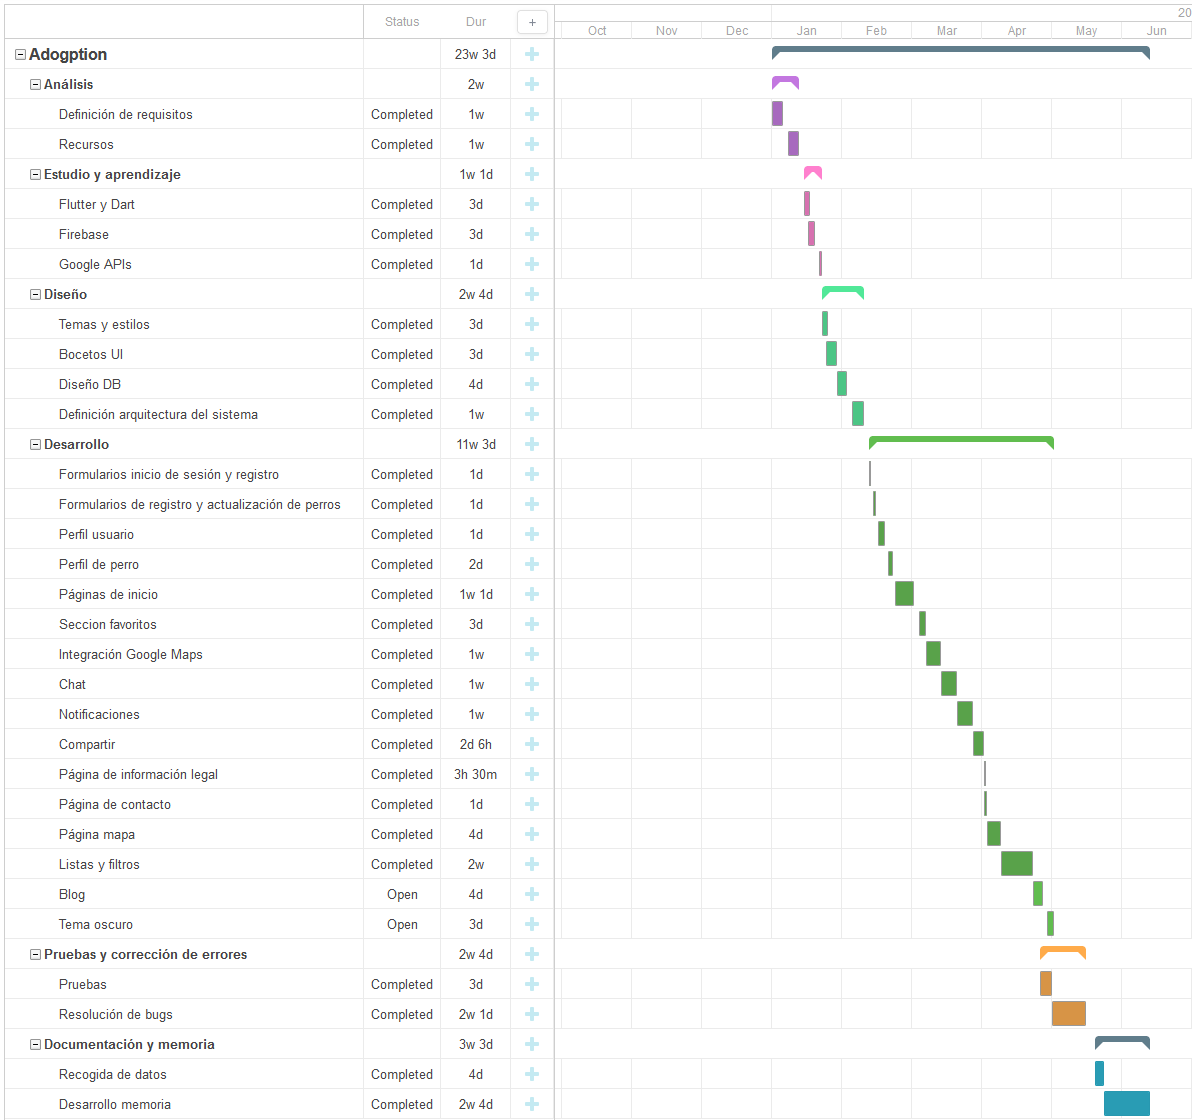
\includegraphics[width=15cm]{GanntSmall2.png}\par}
	\caption{Diagrama de Gannt}
\end{figure}

Dentro del diagrama se pueden ver las diferentes etapas:
\begin{itemize}[noitemsep]
	\item \textbf{Análisis:} Esta etapa consta de unas dos semanas de tiempo, en esta se definen todos los requisitos del sistema y se identifican todos los recursos humanos, de hardware y software necesarios. 
	\item \textbf{Estudio y aprendizaje:} Se destina un breve período previo para aprender a utilizar los lenguajes y servicios que se emplean en el desarrollo de la aplicación.
	\item \textbf{Diseño:} Se reservan casi tres semanas para definir temas, bocetos, diseño de datos y la arquitectura del sistema.
	\item \textbf{Desarrollo:} La etapa más extensa, dividida en secciones para cada funcionalidad a desarrollar a las que se asigna un tiempo adecuado, considerando los servicios y componentes involucrados que definirán su dificultad.
	\item \textbf{Pruebas y corrección de errores:} Una vez completado el desarrollo, es necesario realizar pruebas exhaustivas para identificar errores y faltas de funcionalidades. Se reserva tiempo suficiente para corregir bugs o implementar mejoras de rendimiento si es necesario.
	\item \textbf{Documentación y memoria:} Se dedica un período para recopilar todos los datos y elaborar la memoria en Latex, que documentará el proceso y los resultados obtenidos en las etapas anteriores.
\end{itemize}


% Análisis
\newpage
\section{Análisis}

% Definición y Especificación de Requisitos
\subsection{Definición y especificación de Requisitos}

En esta sección, se detallan los requisitos funcionales y no funcionales identificados para la aplicación que se va a desarrollar. Es esencial definir y comprender estos requisitos para garantizar buenos resultados en el desarrollo y diseño del sistema.

\subsubsection{Requisitos funcionales}

Los requisitos funcionales describen las acciones específicas que el sistema debe realizar, los servicios que debe proporcionar y cómo debe responder a diversas entradas. Estos requisitos se centran en el "qué" del sistema, delineando las funcionalidades clave que los usuarios esperan encontrar en la aplicación.

% RF1
\begin{table}[H]
\captionsetup{justification=raggedright,singlelinecheck=false}
\caption{\textbf{RF1:} Registro de usuarios y protectoras.}
\label{tab:RF1}
	\begin{tabular}{|m{5cm}|m{10cm}|}
	\hline
	\textbf{Datos de Entrada} & Datos ingresados por el usuario en el formulario de registro. Incluyendo datos de contacto, correo electrónico y dirección. \\ 
	\hline
	\textbf{Datos de Salida} & Datos del usuario almacenados en la base de datos. \\ 
	\hline
\end{tabular}
\end{table}

% RF2
\begin{table}[H]
\captionsetup{justification=raggedright,singlelinecheck=false}
\caption{\textbf{RF2:} Registro de caninos.}
\label{tab:RF2}
	\begin{tabular}{|m{5cm}|m{10cm}|}
	\hline
	\textbf{Explicación} & Ofrecer un formulario de registro para añadir perros con características específicas. \\ 
	\hline
	\textbf{Datos de Entrada} & Datos ingresados por la protectora, tales como raza, peso, edad, color y descripción. \\ 
	\hline
	\textbf{Datos de Salida} & Datos del perro almacenados en la base de datos, junto al id de su protectora. \\ 
	\hline
\end{tabular}
\end{table}

% RF3
\begin{table}[H]
\captionsetup{justification=raggedright,singlelinecheck=false}
\caption{\textbf{RF3:} Mostrar listas de usuarios.}
\label{tab:RF23}
	\begin{tabular}{|m{5cm}|m{10cm}|}
	\hline
	\textbf{Explicación} & Mostrar diferentes listas de usuarios en la aplicación, con filtros predeterminados. \\ 
	\hline
	\textbf{Datos de Entrada} & Ninguno. \\ 
	\hline
	\textbf{Datos de Salida} & Listas de usuarios de la aplicación que cumplen con los filtros.  \\ 
	\hline
\end{tabular}
\end{table}

% RF4
\begin{table}[H]
\captionsetup{justification=raggedright,singlelinecheck=false}
\caption{\textbf{RF4:} Mostrar listas de perros.}
\label{tab:RF4}
	\begin{tabular}{|m{5cm}|m{10cm}|}
	\hline
	\textbf{Explicación} & Mostrar diferentes listas de perros en la aplicación, con filtros predeterminados \\ 
	\hline
	\textbf{Datos de Entrada} & Ninguno. \\ 
	\hline
	\textbf{Datos de Salida} & Listas de perros de la aplicación que cumplen con los filtros. \\ 
	\hline
\end{tabular}
\end{table}

% RF5
\begin{table}[H]
\captionsetup{justification=raggedright,singlelinecheck=false}
\caption{\textbf{RF5:} Capacidad de filtrado por propiedades en listas de perros.}
\label{tab:RF5}
	\begin{tabular}{|m{5cm}|m{10cm}|}
	\hline
	\textbf{Explicación} & Proporcionar diferentes filtros para las listas de perros, que corresponden con las diferentes propiedades que puede tener un perro en la aplicación. \\ 
	\hline
	\textbf{Datos de Entrada} & Valores de los filtros proporcionados por el usuario. \\ 
	\hline
	\textbf{Datos de Salida} & Lista de perros de la aplicación que cumplen con los filtros. \\ 
	\hline
\end{tabular}
\end{table}

% RF6
\begin{table}[H]
\captionsetup{justification=raggedright,singlelinecheck=false}
\caption{\textbf{RF6:} Capacidad de filtrado por búsqueda en listas de perros.}
\label{tab:RF6}
	\begin{tabular}{|m{5cm}|m{10cm}|}
	\hline
	\textbf{Explicación} & Filtrar resultados de listas según el texto ingresado en una barra de búsqueda, la búsqueda se realiza en diferentes campos de los perros. \\ 
	\hline
	\textbf{Datos de Entrada} & Texto de búsqueda ingresado por el usuario. \\ 
	\hline
	\textbf{Datos de Salida} &  Lista de perros de la aplicación que cumplen con el criterio de búsqueda en alguno de los campos. \\ 
	\hline
\end{tabular}
\end{table}

% RF7
\begin{table}[H]
\captionsetup{justification=raggedright,singlelinecheck=false}
\caption{\textbf{RF7:} Capacidad de filtrado por búsqueda en listas de usuarios..}
\label{tab:RF7}
	\begin{tabular}{|m{5cm}|m{10cm}|}
\hline
	\textbf{Explicación} & Filtrar resultados de listas según el texto ingresado en una barra de búsqueda, la búsqueda se realiza en diferentes campos de los usuarios. \\ 
	\hline
	\textbf{Datos de Entrada} & Texto de búsqueda ingresado por el usuario. \\ 
	\hline
	\textbf{Datos de Salida} &  Lista de usuarios de la aplicación que cumplen con el criterio de búsqueda en alguno de los campos. \\ 
	\hline
\end{tabular}
\end{table}

% RF8
\begin{table}[H]
\captionsetup{justification=raggedright,singlelinecheck=false}
\caption{\textbf{RF8:}  Proporcionar botón de mapa de resultados en listas de usuarios.}
\label{tab:RF8}
	\begin{tabular}{|m{5cm}|m{10cm}|}
	\hline
	\textbf{Explicación} & Botón en listas de usuarios que redirige a una página con mapa con todos los resultados con ubicación. \\ 
	\hline
	\textbf{Datos de Entrada} & Ninguno \\ 
	\hline
	\textbf{Datos de Salida} & Botón con capacidad de redirección a la página del mapa. \\ 
	\hline
\end{tabular}
\end{table}

% RF9
\begin{table}[H]
\captionsetup{justification=raggedright,singlelinecheck=false}
\caption{\textbf{RF9:} Proporcionar botón de favoritos en perfiles de perros.}
\label{tab:RF9}
	\begin{tabular}{|m{5cm}|m{10cm}|}
	\hline
	\textbf{Explicación} & Permitir a un usuario o protectora marcar como favorito a un perro. \\ 
	\hline
	\textbf{Datos de Entrada} & Click del usuario sobre el botón. \\ 
	\hline
	\textbf{Datos de Salida} & Datos del perro con la actualización de ids de usuarios que lo han marcado/desmarcado como favorito.\\ 
	\hline
\end{tabular}
\end{table}

% RF10
\begin{table}[H]
\captionsetup{justification=raggedright,singlelinecheck=false}
\caption{\textbf{RF10:} Mostrar sección de perros favoritos. }
\label{tab:RF10}
	\begin{tabular}{|m{5cm}|m{10cm}|}
	\hline
	\textbf{Explicación} & Muestra una sección de perros marcados como favoritos en ese momento por el usuario en su página de inicio. \\ 
	\hline
	\textbf{Datos de Entrada} & Ninguno. \\ 
	\hline
	\textbf{Datos de Salida} & Lista horizontal de perros favoritos en la parte inferiro de la página de inicio de los usuarios. \\ 
	\hline
\end{tabular}
\end{table}

% RF11
\begin{table}[H]
\captionsetup{justification=raggedright,singlelinecheck=false}
\caption{\textbf{RF11:} Mostrar adopciones recientes.}
\label{tab:RF11}
	\begin{tabular}{|m{5cm}|m{10cm}|}
	\hline
	\textbf{Explicación} & Muestra un swiper con imágenes de perros marcados como adoptados recientemente. \\ 
	\hline
	\textbf{Datos de Entrada} & Ninguno. \\ 
	\hline
	\textbf{Datos de Salida} & Swiper con imágenes y nombres de perros adoptados en la aplicación. \\ 
	\hline
\end{tabular}
\end{table}

% RF12
\begin{table}[H]
\captionsetup{justification=raggedright,singlelinecheck=false}
\caption{\textbf{RF12:} Proporcionar botón de cerrar sesión.}
\label{tab:RF12}
	\begin{tabular}{|m{5cm}|m{10cm}|}
	\hline
	\textbf{Explicación} & Mostrar botón de cerrar sesión en el menú de acciones en la app bar de la aplicación. \\ 
	\hline
	\textbf{Datos de Entrada} & Ninguno. \\ 
	\hline
	\textbf{Datos de Salida} & Mostrar página de inicio de sesión, después de haber eliminado todos los datos relacionados con el usuario iniciado. \\ 
	\hline
\end{tabular}
\end{table}

% RF13
\begin{table}[H]
\captionsetup{justification=raggedright,singlelinecheck=false}
\caption{\textbf{RF13:} Proporcionar botón de contacto.}
\label{tab:RF13}
	\begin{tabular}{|m{5cm}|m{10cm}|}
	\hline
	\textbf{Explicación} & Mostrar botón de contacto en el menú de acciones en la app bar de la aplicación. \\ 
	\hline
	\textbf{Datos de Entrada} & Ninguno. \\ 
	\hline
	\textbf{Datos de Salida} & Mostrar página de contacto. \\ 
	\hline
\end{tabular}
\end{table}

% RF14
\begin{table}[H]
\captionsetup{justification=raggedright,singlelinecheck=false}
\caption{\textbf{RF14:} Botón de menu lateral en la app bar.}
\label{tab:RF14}
	\begin{tabular}{|m{5cm}|m{10cm}|}
	\hline
	\textbf{Explicación} & Mostrar botón que abre menú lateral. \\ 
	\hline
	\textbf{Datos de Entrada} & Ninguno. \\ 
	\hline
	\textbf{Datos de Salida} & Menu lateral con las páginas disponibles para ese usuario. \\ 
	\hline
\end{tabular}
\end{table}

% RF15
\begin{table}[H]
\captionsetup{justification=raggedright,singlelinecheck=false}
\caption{\textbf{RF15:} Mostrar datos personales en el menú lateral.}
\label{tab:RF15}
	\begin{tabular}{|m{5cm}|m{10cm}|}
	\hline
	\textbf{Explicación} & Muestra los datos del usuario iniciado en el menú lateral. \\ 
	\hline
	\textbf{Datos de Entrada} & Ninguno. \\ 
	\hline
	\textbf{Datos de Salida} & Datos del usuario almacenados en la base de datos. \\ 
	\hline
\end{tabular}
\end{table}

% RF16
\begin{table}[H]
\captionsetup{justification=raggedright,singlelinecheck=false}
\caption{\textbf{RF16:} Botón de 'Inicio' en el menú lateral.}
\label{tab:RF16}
	\begin{tabular}{|m{5cm}|m{10cm}|}
	\hline
	\textbf{Explicación} & Proporcionar botón para redirigir al usuario a la página de inicio de la aplicación. \\ 
	\hline
	\textbf{Datos de Entrada} &  Ninguno. \\ 
	\hline
	\textbf{Datos de Salida} &  Página de inicio de la aplicación. \\ 
	\hline
\end{tabular}
\end{table}

% RF17
\begin{table}[H]
\captionsetup{justification=raggedright,singlelinecheck=false}
\caption{\textbf{RF17:} Botón de 'Perfil personal' en el menú lateral.}
\label{tab:RF17}
	\begin{tabular}{|m{5cm}|m{10cm}|}
	\hline
	\textbf{Explicación} & Proporcionar botón para redirigir al usuario a la página de inicio de la aplicación. \\ 
	\hline
	\textbf{Datos de Entrada} &  Ninguno. \\ 
	\hline
	\textbf{Datos de Salida} &  Página de perfil personal. \\ 
	\hline
\end{tabular}
\end{table}

% RF18
\begin{table}[H]
\captionsetup{justification=raggedright,singlelinecheck=false}
\caption{\textbf{RF18:} Botón de 'Mensajes' en el menú lateral.}
\label{tab:RF18}
	\begin{tabular}{|m{5cm}|m{10cm}|}
	\hline
	\textbf{Explicación} & Proporcionar botón para redirigir al usuario a la página de chats de la aplicación. \\ 
	\hline
	\textbf{Datos de Entrada} &  Ninguno. \\ 
	\hline
	\textbf{Datos de Salida} &  Página de chats. \\ 
	\hline
\end{tabular}
\end{table}

% RF19
\begin{table}[H]
\captionsetup{justification=raggedright,singlelinecheck=false}
\caption{\textbf{RF19:} Botón de 'Protectoras' en el menú lateral.}
\label{tab:RF19}
	\begin{tabular}{|m{5cm}|m{10cm}|}
	\hline
	\textbf{Explicación} & Proporcionar botón para redirigir al usuario a la lista de protectoras de la aplicación. \\ 
	\hline
	\textbf{Datos de Entrada} &  Ninguno. \\ 
	\hline
	\textbf{Datos de Salida} &  Lista de protectoras ya verificadas en la aplicación. \\ 
	\hline
\end{tabular}
\end{table}

% RF20
\begin{table}[H]
\captionsetup{justification=raggedright,singlelinecheck=false}
\caption{\textbf{RF20:} Botón de 'Mis perros' en el menú lateral.}
\label{tab:RF20}
	\begin{tabular}{|m{5cm}|m{10cm}|}
	\hline
	\textbf{Explicación} & Proporcionar botón para redirigir al usuario a la lista de sus perros de la aplicación \\ 
	\hline
	\textbf{Datos de Entrada} &  Ninguno. \\ 
	\hline
	\textbf{Datos de Salida} &  Lista de perros que ha dado de alta el usuario en la aplicación. \\ 
	\hline
\end{tabular}
\end{table}

% RF21
\begin{table}[H]
\captionsetup{justification=raggedright,singlelinecheck=false}
\caption{\textbf{RF21:} Botón de 'Usuarios' en el menú lateral.}
\label{tab:RF21}
	\begin{tabular}{|m{5cm}|m{10cm}|}
	\hline
	\textbf{Explicación} & Proporcionar botón para redirigir al usuario a la lista de usuarios de la aplicación. \\ 
	\hline
	\textbf{Datos de Entrada} &  Ninguno. \\ 
	\hline
	\textbf{Datos de Salida} &  Lista de usuarios que no son protectoras en la aplicación. \\ 
	\hline
\end{tabular}
\end{table}

% RF22
\begin{table}[H]
\captionsetup{justification=raggedright,singlelinecheck=false}
\caption{\textbf{RF22:} Botón de 'Información legal' en el menú lateral.}
\label{tab:RF22}
	\begin{tabular}{|m{5cm}|m{10cm}|}
	\hline
	\textbf{Explicación} & Proporcionar botón para redirigir al usuario a la página de información legal de la aplicación. \\ 
	\hline
	\textbf{Datos de Entrada} &  Ninguno. \\ 
	\hline
	\textbf{Datos de Salida} &  Página de información legal de la aplicación. \\ 
	\hline
\end{tabular}
\end{table}

% RF23
\begin{table}[H]
\captionsetup{justification=raggedright,singlelinecheck=false}
\caption{\textbf{RF23:} Edición de datos personales y de contacto.}
\label{tab:RF23}
	\begin{tabular}{|m{5cm}|m{10cm}|}
	\hline
	\textbf{Explicación} & Proporcionar formularios de edición para los datos del usuario. \\ 
	\hline
	\textbf{Datos de Entrada} & Datos ingresados por el usuario en el formulario. Puede haber datos sin actualizar. \\ 
	\hline
	\textbf{Datos de Salida} &  Datos del usuario actualizados en la base de datos. \\ 
	\hline
\end{tabular}
\end{table}

% RF24
\begin{table}[H]
\captionsetup{justification=raggedright,singlelinecheck=false}
\caption{\textbf{RF24:} Edición de datos de perros.}
\label{tab:RF24}
	\begin{tabular}{|m{5cm}|m{10cm}|}
	\hline
	\textbf{Explicación} & Propocionar formularios de edición para los datos de los caninos. \\ 
	\hline
	\textbf{Datos de Entrada} &  Datos ingresados por el usuario en el formulario. Puede haber datos sin actualizar.  \\ 
	\hline
	\textbf{Datos de Salida} &   Datos del canino actualizados en la base de datos. \\ 
	\hline
\end{tabular}
\end{table}

% RF25
\begin{table}[H]
\captionsetup{justification=raggedright,singlelinecheck=false}
\caption{\textbf{RF25:} Recuperación de contraseña.}
\label{tab:RF25}
	\begin{tabular}{|m{5cm}|m{10cm}|}
	\hline
	\textbf{Explicación} & Proporcionar formularios de recuperación de contraseña para los usuarios y protectoras. \\ 
	\hline
	\textbf{Datos de Entrada} & Correo electrónico ingresado por el usuario. \\ 
	\hline
	\textbf{Datos de Salida} & Correo electrónico con las instrucciones de recuperación de contraseña. \\ 
	\hline
\end{tabular}
\end{table}

% RF26
\begin{table}[H]
\captionsetup{justification=raggedright,singlelinecheck=false}
\caption{\textbf{RF26:} Mostrar página de perfil de usuario/protectora.}
\label{tab:RF26}
	\begin{tabular}{|m{5cm}|m{10cm}|}
	\hline
	\textbf{Explicación} & Proporcionar una interfaz que condense toda la información de un usuario en una sola página. \\ 
	\hline
	\textbf{Datos de Entrada} & Ninguno. \\ 
	\hline
	\textbf{Datos de Salida} & Datos del usuario correspondinte, incluyendo foto de perfil, correo y los perros (si los tiene). Además incluirá el botón de contacto para abir chat. \\ 
	\hline
\end{tabular}
\end{table}

% RF27
\begin{table}[H]
\captionsetup{justification=raggedright,singlelinecheck=false}
\caption{\textbf{RF27:} Mostrar página de perfil de canino.}
\label{tab:RF27}
	\begin{tabular}{|m{5cm}|m{10cm}|}
	\hline
	\textbf{Explicación} & Proporcionar una interfaz que condense toda la información relacionada con un perro en una sola página. \\ 
	\hline
	\textbf{Datos de Entrada} & Ninguno. \\ 
	\hline
	\textbf{Datos de Salida} & Datos del perro correspondiente, incluyendo foto de perfil, características del canino (edad, raza, peso, descripción...). Además de un mapa indicando su ubicación, el bóton de favoritos y de compartir. También incluye el botón de abrir chat. Contendrá los botones de edición si el perro es del usuario que visita el perfil. \\ 
	\hline
\end{tabular}
\end{table}

% RF28
\begin{table}[H]
\captionsetup{justification=raggedright,singlelinecheck=false}
\caption{\textbf{RF28:} Compartir perros a través de enlace.}
\label{tab:RF28}
	\begin{tabular}{|m{5cm}|m{10cm}|}
	\hline
	\textbf{Explicación} & Proporcionar un botón que genere un enlace para redirigir a un usuario al perfil de ese perro en concreto. \\ 
	\hline
	\textbf{Datos de Entrada} & Ninguno. \\ 
	\hline
	\textbf{Datos de Salida} & Url a la aplicación con los parámetros correspondientes para redirigir al perfil de perro. \\ 
	\hline
\end{tabular}
\end{table}

% RF29
\begin{table}[H]
\captionsetup{justification=raggedright,singlelinecheck=false}
\caption{\textbf{RF29:} Página del mapa.}
\label{tab:RF29}
	\begin{tabular}{|m{5cm}|m{10cm}|}
	\hline
	\textbf{Explicación} & Proporcionar una interfaz que contenga un mapa con diferentes marcadores para cada una de las protectoras y un listado de las mismas debajo del mapa. \\ 
	\hline
	\textbf{Datos de Entrada} & Ninguno. \\ 
	\hline
	\textbf{Datos de Salida} & Mapa con marcadores y listado de protectoras, con elementos que pueden mover la cámara a los diferentes marcadores del mapa. \\ 
	\hline
\end{tabular}
\end{table}


% RF30
\begin{table}[H]
\captionsetup{justification=raggedright,singlelinecheck=false}
\caption{\textbf{RF30:} Página de chats.}
\label{tab:RF30}
	\begin{tabular}{|m{5cm}|m{10cm}|}
	\hline
	\textbf{Explicación} & Proporcionar una interfaz que contenga un listado de chats abiertos dentro de la aplicación. \\ 
	\hline
	\textbf{Datos de Entrada} & Ninguno. \\ 
	\hline
	\textbf{Datos de Salida} & Listado de chats disponibles en la aplicación, incluyen una preview del último mensaje y datos del usuario correspondiente. \\ 
	\hline
\end{tabular}
\end{table}


% RF31
\begin{table}[H]
\captionsetup{justification=raggedright,singlelinecheck=false}
\caption{\textbf{RF31:} Enviar mensajes al chat.}
\label{tab:RF31}
	\begin{tabular}{|m{5cm}|m{10cm}|}
	\hline
	\textbf{Explicación} & Permitir mandar mensajes a otro usuario dentro de la aplicación. \\ 
	\hline
	\textbf{Datos de Entrada} & Texto ingresado por el usuario. \\ 
	\hline
	\textbf{Datos de Salida} & Mensaje guardado en la base de datos Se ctualizar la tabla de chats de la base de datos con el último mensaje enviado y generar el id del chat si es el primer mensaje. Notificación al usuario receptor. \\ 
	\hline
\end{tabular}
\end{table}


% RF32
\begin{table}[H]
\captionsetup{justification=raggedright,singlelinecheck=false}
\caption{\textbf{RF32:} Enviar imágenes al chat.}
\label{tab:RF32}
	\begin{tabular}{|m{5cm}|m{10cm}|}
\hline
	\textbf{Explicación} & Permitir mandar mensajes a otro usuario dentro de la aplicación. \\ 
	\hline
	\textbf{Datos de Entrada} & Imagen adjuntada por el usuario. \\ 
	\hline
	\textbf{Datos de Salida} & Imagen guardada además de su referencia en la tabla de mensaje. Se la tabla de chats de la base de datos con el último mensaje enviado y generar el id del chat si es el primer mensaje. Notificación al usuario receptor. \\ 
	\hline
\end{tabular}
\end{table}


% RF33
\begin{table}[H]
\captionsetup{justification=raggedright,singlelinecheck=false}
\caption{\textbf{RF33:} Abrir un chat nuevo.}
\label{tab:RF33}
	\begin{tabular}{|m{5cm}|m{10cm}|}
	\hline
	\textbf{Explicación} & Proporcionar un botón de contacto para abrir un chat con algún usuario dentro de la aplicación. \\ 
	\hline
	\textbf{Datos de Entrada} & Ninguno. \\ 
	\hline
	\textbf{Datos de Salida} & Interfaz del chat, con la cabecera que incluye los datos del usuario receptor. \\ 
	\hline
\end{tabular}
\end{table}

% RF34
\begin{table}[H]
\captionsetup{justification=raggedright,singlelinecheck=false}
\caption{\textbf{RF34:} Borrar un chat.}
\label{tab:RF34}
	\begin{tabular}{|m{5cm}|m{10cm}|}
	\hline
	\textbf{Explicación} & Deslizar un chat para eliminarlo de la lista de chats disponibles \\ 
	\hline
	\textbf{Datos de Entrada} & Ninguno. \\ 
	\hline
	\textbf{Datos de Salida} & Lista actualizada sin el chat que se acaba de eliminar \\ 
	\hline
\end{tabular}
\end{table}

% RF35
\begin{table}[H]
\captionsetup{justification=raggedright,singlelinecheck=false}
\caption{\textbf{RF35:} Marcar/desmarcar perro como adoptado.}
\label{tab:RF35}
	\begin{tabular}{|m{5cm}|m{10cm}|}
	\hline
	\textbf{Explicación} & Proporcionar un botón dentro del perfil del perro que permite a una protectora marcar/desmarcar a un perro de la aplicación como adoptado. \\ 
	\hline
	\textbf{Datos de Entrada} & Estado nuevo según si se quiere marcar o desmarcar. \\ 
	\hline
	\textbf{Datos de Salida} & Perfil del canino actualizado y una etiqueta que indica si está adoptado. \\ 
	\hline
\end{tabular}
\end{table}


% RF36
\begin{table}[H]
\captionsetup{justification=raggedright,singlelinecheck=false}
\caption{\textbf{RF36:} Página de contacto.}
\label{tab:RF36}
	\begin{tabular}{|m{5cm}|m{10cm}|}
	\hline
	\textbf{Explicación} & Proporcionar una interfaz que rehúna datos de contacto de administradores. \\ 
	\hline
	\textbf{Datos de Entrada} & Ninguno. \\ 
	\hline
	\textbf{Datos de Salida} & Interfaz que incluye correo electrónico y un botón de contacto para abrir un chat con un administrador. \\ 
	\hline
\end{tabular}
\end{table}

% RF37
\begin{table}[H]
\captionsetup{justification=raggedright,singlelinecheck=false}
\caption{\textbf{RF37:} Página de información legal.}
\label{tab:RF37}
	\begin{tabular}{|m{5cm}|m{10cm}|}
	\hline
	\textbf{Explicación} & Proporcionar una interfaz que rehúna toda la información legal y advertencias. \\ 
	\hline
	\textbf{Datos de Entrada} & Ninguno. \\ 
	\hline
	\textbf{Datos de Salida} & Interfaz que incluye toda la información legal de la aplicación. \\ 
	\hline
\end{tabular}
\end{table}

% RF38
\begin{table}[H]
\captionsetup{justification=raggedright,singlelinecheck=false}
\caption{\textbf{RF38:} Proporcionar página de inició según rol.}
\label{tab:RF38}
	\begin{tabular}{|m{5cm}|m{10cm}|}
	\hline
	\textbf{Explicación} & Proporcionar una interfaz única según el rol después de iniciar sesión. \\ 
	\hline
	\textbf{Datos de Entrada} & Correo electrónico y contraseña para iniciar sesión. \\ 
	\hline
	\textbf{Datos de Salida} & Página de inicio que varía según el rol. \\ 
	\hline
\end{tabular}
\end{table}

% RF39
\begin{table}[H]
\captionsetup{justification=raggedright,singlelinecheck=false}
\caption{\textbf{RF39:} Página de administrador.}
\label{tab:RF39}
	\begin{tabular}{|m{5cm}|m{10cm}|}
	\hline
	\textbf{Explicación} & Proporcionar una página para los administradores. \\ 
	\hline
	\textbf{Datos de Entrada} & Correo electrónico y contraseña de administrador para iniciar sesión. \\ 
	\hline
	\textbf{Datos de Salida} & Interfaz para los administradores, que incluye listas con diferentes filtros de usuarios y caninos para manejar usuarios y caninos. \\ 
	\hline
\end{tabular}
\end{table}

% RF40
\begin{table}[H]
\captionsetup{justification=raggedright,singlelinecheck=false}
\caption{\textbf{RF40:} Búsqueda de direcciones.}
\label{tab:RF40}
	\begin{tabular}{|m{5cm}|m{10cm}|}
	\hline
	\textbf{Explicación} & Proporcionar una barra de búsqueda de direcciones para facilitar la introducción de datos. \\ 
	\hline
	\textbf{Datos de Entrada} & Una cadena de caracteres que puede contener el nombre de la calle, la ciudad, el código postal... \\ 
	\hline
	\textbf{Datos de Salida} & Un listado de direcciones que coinciden con la búsqueda, al seleccionar una, se autocompletan los datos del formulario. \\ 
	\hline
\end{tabular}
\end{table}

% RF41
\begin{table}[H]
\captionsetup{justification=raggedright,singlelinecheck=false}
\caption{\textbf{RF41:} Cambiar a tema oscuro.}
\label{tab:RF41}
	\begin{tabular}{|m{5cm}|m{10cm}|}
	\hline
	\textbf{Explicación} & Proporcionar una barra de búsqueda de direcciones para facilitar la introducción de datos. \\ 
	\hline
	\textbf{Datos de Entrada} & Ninguno.\\ 
	\hline
	\textbf{Datos de Salida} & Interfaz con el tema oscuro.  \\ 
	\hline
\end{tabular}
\end{table}

% RF42
\begin{table}[H]
\captionsetup{justification=raggedright,singlelinecheck=false}
\caption{\textbf{RF42:} Subir post al blog.}
\label{tab:RF42}
	\begin{tabular}{|m{5cm}|m{10cm}|}
	\hline
	\textbf{Explicación} & Permitir a un usuario subir un post al blog. \\ 
	\hline
	\textbf{Datos de Entrada} & Contenido que puede ser texto o imágenes. \\ 
	\hline
	\textbf{Datos de Salida} & Post publicado en el blog de la aplicación. \\ 
	\hline
\end{tabular}
\end{table}

% RF43
\begin{table}[H]
\captionsetup{justification=raggedright,singlelinecheck=false}
\caption{\textbf{RF43:} Comentar post del blog.}
\label{tab:RF43}
	\begin{tabular}{|m{5cm}|m{10cm}|}
	\hline
	\textbf{Explicación} & Permitir a un usuario comentar un post en el blog. \\ 
	\hline
	\textbf{Datos de Entrada} & Texto que puede incluir emoticonos. \\ 
	\hline
	\textbf{Datos de Salida} & Comentario publicado en el post. \\ 
	\hline
\end{tabular}
\end{table}


\subsubsection{Requisitos no funcionales}

Los requisitos no funcionales son los encargados de ofrecer al usuario una experiencia robusta y óptima a lo largo de la aplicación. Para el desarrollo de la aplicación se han tenido en cuenta los siguientes puntos:

\begin{itemize}[noitemsep]
	\item \textbf{Rendimiento:} La aplicación debe ser capaz de responder rápidamente a las interacciones de los usuarios y ejecutar las operaciones en un breve período de tiempo. 
		\begin{itemize}[noitemsep]
			\item Se propone una deadline de 3 segundos como tiempo óptimo para cargar una página completa.
			\item El tiempo de respuesta del servidor se espera que sea menor de 2 segundos.
			\item Se espera que la aplicación sea capaz de manejar múltiples peticiones sin que se produzca una degradación perceptible del rendimiento. Se propone como deadline 10000 de solicitudes.
			\item Se espera que la base de datos realice consultas simples y complejas en menos de un segundo.
			\item Se propone que en el caso de búsquedas y filtrados el tiempo de procesamiento puede ser mayor de 3 segundos, pero menor de 6.
			\item La aplicación denbe poder manejar alrededor de 10000 usuarios de forma concurrente sin sufrir degradación de rendimiento.
		\end{itemize}
	\item \textbf{Escalabilidad:} Es necesario que a la hora de implementar código, se mantenga un código en el que sea sencillo añadir o quitar funcionalidades sin comprometer el comportamiento de la aplicación.
		\begin{itemize}[noitemsep]
			\item Los componentes de la aplicación deben estar claramente definidos y documentados.
			\item Un componente base debe recoger todas las propiedades comunes que pueden tener ese tipo de componentes. Por ejemplo, un componente base para los botones, deberá recoger el tamaño de la fuente, la forma del botón, colores etc.
			\item Las funcionalidades desarrolladas deben ser fácilmente deprecadas si es necesario, es decir, no deben depender unas de otras si no es estrictamente necesario.
			\item Los nuevos componentes que se desarrollen no deben afectar el funcionamiento de la aplicación.
			\item Se espera que si fuera necesario actualizar algún componente en la UI, actualizando el componente base se actualicen todos los componentes de ese tipo.
		\end{itemize}
	\item \textbf{Usabilidad:} Para esta aplicación, que tiene un rango de usuarios muy amplio, se espera que un usuario poco experimentado sea capaz de usar la aplicación de forma sencilla. La aplicación debe proporcionar una interfaz intuitiva y atractiva. 
		\begin{itemize}[noitemsep]
			\item La interfaz debe ser limpia y organizada.
			\item Los colores de la aplicación deben ser coherentes.
			\item La navegación de la aplicación debe cumplir la norma de los tres clicks, "\textit{cualquier persona que visite la aplicación debería alcanzar la información más crítica como máximo en tres clics}".
			\item La aplicación deberá ser lo suficientemente intuitiva o proporcionar guía de uso si es necesario.
			\item Se espera que la aplicación sea testeada por usuarios reales antes del primer despliegue para posibles correciones.
		\end{itemize}
	\item \textbf{Confiabilidad:} Para la aplicación, se espera que haya un correcto manejo de errores.
		\begin{itemize}[noitemsep]
			\item Se espera que un usuario sea informado con un mensaje adecuado si ocurre un error crítico.
			\item Durante el desarrollo es necesario testear para poder añadir mecanismos que minimicen los errores conocidos en la aplicación.
			\item Las copias de seguridad son indispensables para garantizar que no se pierden los datos ante un error crítico.
			\item Se propone añadir mecanismos de manejo de errores en todas las operaciones críticas (lectura y escritura)  para evitar errores críticos.
		\end{itemize}
	\item \textbf{Seguridad:} Para garantizar este requisito, la aplicación debe proteger los datos de los usuarios y prevenir accesos no autorizados. También, en este caso en concreto, es necesario garantizar en medida de los posible, que toda la información que se dé de alta, sea real y fehaciente.
		\begin{itemize}[noitemsep]
			\item Las contraseñas o datos sensibles no pueden estar expuestos, se deben almacenar con cifrados.
			\item La aplicación no va a permitir el acceso a usuarios que no tengan una cuenta.
			\item La aplicación no va a permitir dar de alta a perros a las protectoras que no estén verificadas por administradores, para evitar casos fraudulentos.
			\item Un administrador tiene acceso a diferentes listas en las que puede verificar información y tiene la libertad de eliminar lo que crea correspondiente.
			\item Debe prevenirse con mecanismos para ataques comunes como pueden ser las inyecciones SQL, CSS, Y CSRF. 
		\end{itemize}
	\item \textbf{Documentación:} A lo largo de todas las etapas, se almacenará toda la información relevante, ya sea en el código, en documentos aparte o en la propia memoria.
\end{itemize}

\subsection{Diagramas de casos de uso}


%Caso de uso: Iniciar sesión
\begin{figure}[H]
	\begin{center}
		{
\includegraphics[width=12cm]{White.png}\par}
		\caption{Caso de uso: iniciar sesión.}
	\end{center}
\end{figure}


%Caso de uso: Registro
\begin{figure}[H]
	\begin{center}
		{
\includegraphics[width=12cm]{White.png}\par}
		\caption{Caso de uso: registro.}
	\end{center}
\end{figure}


%Caso de uso: Recuperar contraseña
\begin{figure}[H]
	\begin{center}
		{
\includegraphics[width=12cm]{White.png}\par}
		\caption{Caso de uso: recuperar contraseña.}
	\end{center}
\end{figure}


%Caso de uso: Gestionar perfil usuario
\begin{figure}[H]
	\begin{center}
		{
\includegraphics[width=12cm]{White.png}\par}
		\caption{Caso de uso: gestionar perfil de usuario.}
	\end{center}
\end{figure}



%Caso de uso: Gestionar perfil de perro
\begin{figure}[H]
	\begin{center}
		{
\includegraphics[width=12cm]{White.png}\par}
		\caption{Caso de uso: gestionar perfil de perro.}
	\end{center}
\end{figure}


%Caso de uso: Listas de perros
\begin{figure}[H]
	\begin{center}
		{
\includegraphics[width=12cm]{White.png}\par}
		\caption{Caso de uso: listas de perros.}
	\end{center}
\end{figure}


%Caso de uso: Listas de usuario
\begin{figure}[H]
	\begin{center}
		{
\includegraphics[width=12cm]{White.png}\par}
		\caption{Caso de uso: listas de usuarios.}
	\end{center}
\end{figure}


%Caso de uso: Mensajes
\begin{figure}[H]
	\begin{center}
		{
\includegraphics[width=12cm]{White.png}\par}
		\caption{Caso de uso: mensajería.}
	\end{center}
\end{figure}

%Caso de uso: Notificaciones
\begin{figure}[H]
	\begin{center}
		{
\includegraphics[width=12cm]{White.png}\par}
		\caption{Caso de uso: notificaciones}
	\end{center}
\end{figure}




% Recursos
\subsection{Recursos}

En esta sección se definen todos los recursos necesarios para el desarrollo de la aplicación.

\subsubsection{Recursos humanos}

En este proyecto, solo va a intervenir una persona, la autora de la memoria. Se trata de una Ingeniera de Software (semi-senior). Esta persona es encargada de cumplimentar todos los aspectos del desarrollo. El horario laboral será de Lunes a Viernes de media jornada.


\subsubsection{Hardware}

Para este proyecto, el hardware es un ordenador de sobremesa personal y una tablet android.

\begin{itemize}[noitemsep]
	\item Ordenador de sobremesa, para el desarrollo y las pruebas, con los siguientes componentes:
		\begin{itemize}[noitemsep]
			\item \textbf{Procesador:} AMD Ryzen 7 3700X 8-Core Processor - 3.60 GHz
			\item \textbf{Memoria RAM:} DDR4 3000 2x16GB
			\item \textbf{Tarjeta gráfica:} NVIDIA GeForce GTX 1660 SUPER
			\item \textbf{Placa base:} ASUS TUF GAMING B550-PLUS WIFI II
			\item \textbf{Disipador:} Noctua NH-D15
		\end{itemize}
	\item Tablet android Hi9plus, para realizar pruebas en un dispositivo android físico.
\end{itemize}

\subsubsection{Software}

El sistema operativo utilizado es el que estaba instalado previamente en el ordenador personal.

Para escoger el framework que se va a utilizar en el proyecto partimos de la base de que vamos a realizar una aplicación android. Existen diferentes frameworks como \textit{React Native}, \textit{Flutter}, \textit{Kotlin Multiplatform} etc. que ofrecen integración con android para facilitar el desarrollo. En este proyecto, se ha optado por desarrollar con Flutter, debido a que se ha trabajado previamente con él. Este framework, además, permite realizar un desarrollo multiplataforma y ofrece un alto rendimiento. 

El lenguaje utilizado es \textit{Dart}, este lenguaje es muy similar a Java, se trata de un lenguaje orientado a objetos y se utiliza prinicpalmente para el desarrollo de aplicaciones del lado del cliente. Es un lenguaje bastante popularizado, uno de los motivos para optar por este lenguaje es el manenimiento que recibe a día de hoy y por la simple que resulta para programar. Para añadir funcionalidades extra, se han escogido varias bibiliotecas que ofrecen algunos microservicios o widgets.

Por último, para manejar la base de datos, se ha optado por usar \textit{Firebase}. Se trata de una plataforma de desarrollo de aplicaciones web muy popularizada, también desarrollada por Google. Ofrece diferentes servicios para la autenticación, el hosting de la aplicación y bases de datos en tiempo real, eso lo convertia en el candidato adecuado para manejar el chat, la funcionalidad de compartir y otras cosas funcionalidades que nuestra aplicación requiere.

\begin{itemize}[noitemsep]
	\item \textbf{Sistema Operativo:} Windows 11 x64
	\item \textbf{IDE:} Android Studio Hedgehog | 2023.1.1 Patch 2
	\item \textbf{Framework:} Flutter 3.19.0 -  \href{https://flutter.dev/6}{Flutter DEV} \cite{flutter_dev}
	\item \textbf{Lenguaje:} Dart 3.3.0 - \href{https://dart.dev/}{Dart DEV} \cite{dart_dev}
	\item \textbf{Paquetes:}
		\begin{itemize}[noitemsep]
		  \item \texttt{cupertino\_icons: \^{}1.0.2}
		  \item \texttt{firebase\_core: \^{}2.24.2}
		  \item \texttt{firebase\_database: \^{}10.3.8}
		  \item \texttt{firebase\_storage:}
		  \item \texttt{cloud\_firestore: \^{}4.13.6}
		  \item \texttt{firebase\_auth: \^{}4.15.3}
		  \item \texttt{responsive\_sizer: \^{}3.3.0+1}
		  \item \texttt{flutter\_login: \^{}5.0.0}
		  \item \texttt{google\_fonts: \^{}4.0.4}
		  \item \texttt{resize: \^{}1.0.0}
		  \item \texttt{awesome\_notifications: \^{}0.9.2}
		  \item \texttt{csc\_picker: \^{}0.2.7}
		  \item \texttt{map\_address\_picker: \^{}0.3.5}
		  \item \texttt{geocoding: \^{}3.0.0}
		  \item \texttt{search\_map\_location: 0.0.6}
		  \item \texttt{image\_picker: \^{}1.0.7}
		  \item \texttt{image\_cropper: \^{}4.0.1}
		  \item \texttt{path\_provider: \^{}2.1.2}
		  \item \texttt{flutter\_image\_compress: \^{}2.1.0}
		  \item \texttt{address\_form: \^{}0.0.2}
		  \item \texttt{address: \^{}0.1.0+2}
		  \item \texttt{google\_maps\_webservice: \^{}0.0.20-nullsafety.5}
		  \item \texttt{meta\_validator: \^{}0.0.2}
		  \item \texttt{geolocator: \^{}9.0.2}
		  \item \texttt{dropdown\_search: \^{}5.0.6}
		  \item \texttt{card\_swiper: \^{}3.0.1}
		  \item \texttt{filter\_list: \^{}1.0.2}
		  \item \texttt{flutter\_filter\_dialog: \^{}1.2.0}
		  \item \texttt{choice: \^{}2.3.2}
		  \item \texttt{animate\_gradient: \^{}0.0.2+1}
		  \item \texttt{firebase\_messaging: \^{}14.9.1}
		  \item \texttt{flutter\_chat\_bubble: \^{}2.0.2}
		  \item \texttt{chat\_bubbles: \^{}1.6.0}
		  \item \texttt{share\_plus: \^{}9.0.0}
		  \item \texttt{app\_links: \^{}6.0.1}
		  \item \texttt{url\_launcher: \^{}6.2.6}
		  \item \texttt{firebase\_dynamic\_links: \^{}5.5.4}
		  \item \texttt{go\_router: \^{}14.0.2}
		  \item \texttt{get: \^{}4.6.6}
		  \item \texttt{linkwell: \^{}2.0.6}
		  \item \texttt{toastification: \^{}1.0.0}
		\end{itemize}
	\item \textbf{Base de datos:} Firebase database - \href{https://console.firebase.google.com}{Firebase console} \cite{firebase_console}
\end{itemize}


\subsection{Costes}

Habiendo escogido todos los recursos necesarios para el desarrollo del producto, se pueden definir un presupuesto que englobe todos los apartados.

\subsubsection{Recursos humanos}

Para calcular el costo relacionado con el personal, se toma como referencia el sueldo medio de un programador junior, que ronda los \textit{24.000€} anuales, lo que equivale a \textit{12.000€} a media jornada. Haciendo cálculos, al mes corresponden unos \textit{1.000€}. Dado que la duración del proyecto es de 5 meses y medio, el costo total en salarios para el empleado será de \textit{5.500€}.

\subsubsection{Hardware}

Debido a que el equipo utilizado no es nuevo, se consideran los gastos del equipo teniendo en cuenta que un equipo informático se puede amortizar hasta 8 años. El precio aproximado del ordenador es de unos \textit{1000€}. Un año tiene 12 meses, lo que resulta en 96 meses en total de amortización, lo que implica que cuesta unos \textit{11€} al mes. Dado que la duración del proyecto es de 5 meses y medio, el costo del ordenador sería de \textit{60,50€} en total. El precio de la tablet es de unos \textit{100€}, así que utilizando los mismos cálculos, el costo de la tablet es de \textit{5,72€} en total.

\subsubsection{Software}

Para el alcance de este proyecto y los números a los que se aspira, al menos durante la primera fase, se ha optado por utilizar las versiones gratuitas del software escogido, lo que resulta en un coste total de 0€ en software.

\begin{itemize}[noitemsep]
	\item Firebase - Plan Spark - \href{https://firebase.google.com/pricing?hl=es-419}{Guía de planes} \cite{firebase_plans}
	\item Google APIs - Ofrecen créditos gratuitos de hasta \textit{200€} para cubir los gastos que se generen por el uso de la API. - \href{https://mapsplatform.google.com/intl/es/pricing/}{Precios}\cite{google_prices}
	\item IDE + Framework - Gratuitos
\end{itemize}


\subsubsection{Otros}

Debido a que el desarrollo del proyecto se realiza en la casa de la persona empleada, se añaden a los costes la electricidad usada. Usando como referencia el gasto mensual de electricidad, que ronda los \textit{30€}.

\begin{table}[H]
    \centering
    \begin{tabular}{ | m{5cm} | m{5cm} | }
	    \hline \textbf{Recurso} & \textbf{Coste (€)} \\ \hline
	    	Personal & 5.500 \\ \hline
	    	\multirow{2}{*}{Hardware} & Ordenador - 60,50 \\& Tablet - 5,72 \\ \hline
	    	Software & 0 \\ \hline
		Electricidad & 180 \\ \hline
	    \textbf{Total} & \textbf{5.746,22€} \\ \hline
    \end{tabular}
    \caption{Costes del proyecto}
    \label{tab:costes}
\end{table}

% Diseño
\newpage
\section{Diseño}

En esta partese incluye toda la estructura de la aplicación, tanto como la interfaz de usuario, el backend y la base de datos.

\subsection{Diseño de base de datos}

Esta sección es primordial para generar unas bases sólidas para la aplicación. Se deben almacenar todas las entidades y todas sus propiedades, definiendo claramente el tipo de cada una.

\subsubsection{Direcciones}

Para todas las protectoras, es necesario almacenar la dirección en la que están ubicadas. Esta información es crucial para mostrar a los usuarios la ubicación de cada protectora y generar marcadores en el mapa correspondiente. Por un lado, se almacenan todas las partes de la dirección, como la ciudad, la calle, el código postal, etc. Por otro lado, cuando un usuario introduzca su dirección, se generarán automáticamente las coordenadas de esa dirección para almacenarlas también, evitando tener que calcularlas cada vez que se carguen los mapas en la interfaz. Asimismo, cuando un usuario actualice su dirección, se actualizarán también sus coordenadas correspondientes en la base de datos.

Para todas las direcciónes se genera una entrada en el que su ID corresponde con el del usuario al que pertenece.

% Addresses
\begin{table}[H]
\captionsetup{justification=raggedright,singlelinecheck=false}
\caption{\textbf{Tabla: addresses}}
\label{tab:Addresses}
	\begin{tabular}{|m{3cm}|m{2cm}|m{5cm}|m{3cm}|}
	\hline
	\textbf{Campo} & \textbf{Tipo} & \textbf{Dato} & \textbf{Obligatorio} \\ 
	\hline
	\textbf{city} & cadena & Ciudad de la dirección & Si \\ 
	\hline
	\textbf{country} & cadena & País de la dirección (España siempre) & Si\\ 
	\hline
	\textbf{province} &  cadena & Provincia de la dirección & Si \\ 
	\hline
	\textbf{street} &  cadena & Calle de la dirección & Si \\ 
	\hline
	\textbf{street\_number} &  cadena & Número de la calle & No\\ 
	\hline
	\textbf{zipcode} & cadena & Código postal & Si \\ 
	\hline
	\textbf{lat} & número & Latitud & Si \\ 
	\hline
	\textbf{lng} & número & Longitud & Si \\ 
	\hline
\end{tabular}
\end{table}

Aqui se muestra un ejemplo real de una dirección almacenada en la base de datos.

\begin{verbatim}
{
  "city": "Murcia",
  "country": "España",
  "lat": 37.9879153,
  "lng": -1.1315578,
  "province": "Murcia",
  "street": "Calle Maestro Alonso",
  "street_number": "4",
  "zipcode": "30005"
}
\end{verbatim}

\subsubsection{Chats}

Para la tabla de chats, se ha decidido almacenar los IDs de los usuarios implicados, aparte se almacena un array de IDs que indica para quien está disponible el chat en ese momento. Al igual que en otras aplicaciones de mensajería, cuando se elimina un chat, éste simplemente desaparece para el usuario que lo borra esto hace que la propiedad de quién puede acceder al chat en ese momento sea modificada. En esta primera iteración del proyecto, los mensajes no se borran. Por ejemplo, si una persona A borra su chat con la persona B y luego vuelve a abrir un chat con esa misma persona, los mensajes anteriores seguirán estando disponibles. En la fase de implementación, se profundizará más en el comportamiento definido para este aspecto.

Almacenar aqui los IDs de los usuarios implicados, permite que si se proponen chats de grupo, sea más sencillo escalarlo, ya que en esta forma la base de datos ya lo está soportando. Lo mismo ocurre con la propiedad que hace referencia a que usuarios pueden ver el chat. 

Para todos los chats se genera un ID automático, al que se hace referencia desde la tabla de usuarios.

% Chats
\begin{table}[H]
\captionsetup{justification=raggedright,singlelinecheck=false}
\caption{\textbf{Tabla: chats}}
\label{tab:chats}
	\begin{tabular}{|m{3cm}|m{2cm}|m{5cm}|m{3cm}|}
	\hline
	\textbf{Campo} & \textbf{Tipo} & \textbf{Dato} & \textbf{Obligatorio} \\ 
	\hline
	\textbf{availableTo} & array & IDs de Usuarios que tienen el chat visible en su página & Si \\ 
	\hline
	\textbf{lastMessage} & cadena & ID del último mensaje mandado en el chat & Si\\ 
	\hline
	\textbf{users} &  array & IDs de Usuarios que intervienen en el chat & Si \\ 
	\hline
\end{tabular}
\end{table}

Aqui se muestra un ejemplo real de un chat almacenado en la base de datos. 

\begin{verbatim}
{
  "availableTo": [
    "kuaKjc6XoiVot1rMeGqBySA5pE13",
    "buO4Vkazs3O2oVKetugxrvTfRw12"
  ],
  "lastMessage": "BaKmuuo8debUTdSNsvw0",
  "users": [
    "kuaKjc6XoiVot1rMeGqBySA5pE13",
    "buO4Vkazs3O2oVKetugxrvTfRw12"
  ]
}
\end{verbatim}

\subsubsection{Perros}

Esta entidad es una de las más importantes de la aplicación, ya que es la que se principal afectada por la mayoría de funcionalidades que se proponen. Principalmente esta tabla contendrá todas las propiedades de los perros que se van a manejar dentro de la app, aunque hay algunas consideraciones importantes para algunas de ellas.

Para el género se han propuesto dos valores fijos que luego se transformaran en la cadena correspondiente cuando se carguen en la UI. Los valores son \textbf{male} y \textbf{female}. Se propone esta solución para cuando se decida añadir traducciones en la aplicación y no trabajar con palabras en español en la base de datos.

Para almacenar la edad, se ha optado por almacenarla junto a las unidades, ya que así se le da la posibilidad al usuario a especificar mejor la edad del perro (el caso de uso es muy concreto, pero añade valor). Los valores de las unidades serán fijos, pudiendo ser:

\begin{itemize}[noitemsep]
	\item \textbf{Meses}
	\item \textbf{Años}
\end{itemize}

Lo mismo ocurre con el peso, se opta por almacenar el peso junto con las unidades para facilitar al usuario especificar el peso. A pesar de que se pueda especificar las unidades del peso, el peso en la base de datos siempre será tratado como KG, para facilitar el uso de los filtros, cuando se traiga a la UI, se actualizará al valor real que corresponda. Las unidades disponibles serán
\begin{itemize}[noitemsep]
	\item \textbf{Gramos}
	\item \textbf{KG}
\end{itemize}

En una primera instancia se propuso almacenar los perros favoritos en la tabla de usuarios, pero tras hacer algunas pruebas se optó por este modelo finalmente. Almacenar los usuarios que han marcado al perro como favorito, facilita las actualizaciones en tiempo real de los resultados de perros.

Para todos los perros se genera un ID automático.

\begin{table}[H]
\captionsetup{justification=raggedright,singlelinecheck=false}
\caption{\textbf{Tabla: dogs}}
\label{tab:dogs}
	\begin{tabular}{|m{3cm}|m{2cm}|m{5cm}|m{3cm}|}
	\hline
	\textbf{Campo} & \textbf{Tipo} & \textbf{Dato} & \textbf{Obligatorio} \\ 
	\hline
	\textbf{adopted} & booleano & Indica si el perro ha sido adoptado. & Si \\ 
	\hline
	\textbf{age} & número & Edad & Si \\ 
	\hline
	\textbf{ageUds} & cadena & Unidades de la edad & Si \\ 
	\hline
	\textbf{breed} & cadena & Raza & Si \\ 
	\hline
	\textbf{castrated} & booleano & Indica si está castrado & Si \\ 
	\hline
	\textbf{color} & cadena & Color & Si \\ 
	\hline
	\textbf{created} & marca de tiempo & Fecha y hora de cuando se ha dado de alta & Si \\ 
	\hline
	\textbf{description} & cadena & Descripción & No \\ 
	\hline
	\textbf{favoriteBy} & array & IDs de usuarios que lo han marcado como favorito & No \\ 
	\hline
	\textbf{forAdoption} & booleano & Indica si está disponible para adopción & No \\ 
	\hline
	\textbf{forFoster} & booleano & Indica si está disponible para acogida & No \\ 
	\hline
	\textbf{gender} & cadena & Género & Si \\ 
	\hline
	\textbf{name} & cadena & Nombre & Si \\ 
	\hline
	\textbf{ownerId} & cadena & ID del propietario & Si \\ 
	\hline
	\textbf{profilePic} & cadena & URL de la imagen de perfil de la mascota & No \\ 
	\hline
	\textbf{weight} & número & Peso & Si \\ 
	\hline
	\textbf{weightUds} & cadena & Unidades de peso & Si \\ 
	\hline
\end{tabular}
\end{table}

Aquí se muestra un ejemplo real de un perro almacenado en la base de datos.

\begin{verbatim}
{
  "adopted": false,
  "age": 1,
  "ageUds": "Años",
  "breed": "Breed 2",
  "castrated": true,
  "color": "Color 1",
  "created": "23 de abril de 2024, 10:56:48 a.m. UTC+2",
  "description": "",
  "favoriteBy": [],
  "forAdoption": true,
  "forFoster": true,
  "gender": "female",
  "name": "Katrina",
  "ownerId": "S4wXwckahiSOLI0Q3exXDVRh2yl2",
  "profilePic": "",
  "weight": 1,
  "weightUds": "KG"
}
\end{verbatim}

\subsubsection{Mensajes}

Aparte de almacenar toda la información de los chats, hay que almacenar los mensajes que se mandan en los chats. Aparte de guardar el contenido del mensaje, se propone hacer una diferenciación por tipos, habiendo en esta primera iteración solo dos tipos, que son: \textbf{default} e \textbf{image}, indicando que un mensaje es texto o imagen respectivamente. Esta definición de tipos ayudará a saber como cargar el contenido en la interfaz.

Para todos los mensajes se genera un ID automático que se puede referenciar desde la tabla de chats.

% Mensajes
\begin{table}[H]
\captionsetup{justification=raggedright,singlelinecheck=false}
\caption{\textbf{Tabla: messages}}
\label{tab:messages}
	\begin{tabular}{|m{3.2cm}|m{2cm}|m{5cm}|m{3cm}|}
	\hline
	\textbf{Campo} & \textbf{Tipo} & \textbf{Dato} & \textbf{Obligatorio} \\ 
	\hline
	\textbf{chatId} & cadena & ID del chat & Si \\ 
	\hline
	\textbf{from} & cadena & ID del emisor del mensaje & Si \\ 
	\hline
	\textbf{messageContent} & cadena & Contenido del mensaje & Si \\ 
	\hline
	\textbf{read} & booleano & Indica si el recpetor a leído el mensaje & Si \\ 
	\hline
	\textbf{sent} & marca de tiempo & Fecha y hora en la que se mandó el mensaje & Si \\ 
	\hline
	\textbf{to} & cadena & ID del receptor del mensaje & Si \\ 
	\hline
	\textbf{type} & cadena & Tipo del mensaje & Si \\ 
	\hline
	\end{tabular}
\end{table}

Aqui se muestra un ejemplo real de una dirección almacenada en la base de datos.

\begin{verbatim}
{
  "chatId": "Sm1Ji0chb9uhofa20VW5",
  "from": "kuaKjc6XoiVot1rMeGqBySA5pE13",
  "messageContent": "Hola, ¿estás?",
  "read": true,
  "sent": "6 de mayo de 2024, 1:57:30 a.m. UTC+2",
  "to": "buO4Vkazs3O2oVKetugxrvTfRw12",
  "type": "default"
}
\end{verbatim}


\subsubsection{Notificaciones}

Cuando un usuario envíe un mensaje, el usuario receptor debe recibir una notificación. Para gestionar las notificaciones de los mensajes, se ha decidido crear una tabla que contenga las solicitudes de notificación para un usuario específico. Al iniciar sesión, se agrega un listener que escucha todos los cambios en esta tabla y cuando llega una nueva solicitud, se envía una notificación a través del canal correspondiente. Cuando el usuario receptor recibe la notificación, esta solicitud se marca como vista. 

Para cada una de las entradas su ID corresponde con el del usuario al que pertenece.

% notifications
\begin{table}[H]
\captionsetup{justification=raggedright,singlelinecheck=false}
\caption{\textbf{Tabla: notifications}}
\label{tab:notifications}
	\begin{tabular}{|m{3.2cm}|m{2cm}|m{5cm}|m{3cm}|}
	\hline
	\textbf{Campo} & \textbf{Tipo} & \textbf{Dato} & \textbf{Obligatorio} \\ 
	\hline
	\textbf{requests} & collection & Colección de peticiones & Si \\ 
	\hline
	\end{tabular}
\end{table}

Para cada petición se genera un ID y se genera en un formato en concreto.

% requests
\begin{table}[H]
\captionsetup{justification=raggedright,singlelinecheck=false}
\caption{\textbf{Tabla: requests}}
\label{tab:requests}
	\begin{tabular}{|m{3.2cm}|m{2cm}|m{5cm}|m{3cm}|}
	\hline
	\textbf{Campo} & \textbf{Tipo} & \textbf{Dato} & \textbf{Obligatorio} \\ 
	\hline
	\textbf{chats} & array & IDs de los chats que pertenecen al usuario & Si \\ 
	\hline
	\textbf{email} & cadena &  ID del chat desde el que se manda la notificación & Si \\ 
	\hline
	\textbf{profilePic} & cadena & URL de la imagen de foto de perfil & Si \\ 
	\hline
	\textbf{rol} & cadena & Rol del usuario & Si \\ 
	\hline
	\textbf{username} & cadena & Nombre de usuario & Si \\ 
	\hline
	\textbf{verified} & cadena & Indica si ha sido verificado por un administrador & Si, solo si el rol es company \\ 
	\hline
	\end{tabular}
\end{table}


Aqui se muestra una petición real almacenada en la base de datos.

\begin{verbatim}
{
  "body": "Hola, ¿cómo estás?",
  "chatId": "Sm1Ji0chb9uhofa20VW5",
  "new": false,
  "summary": "Hola, ¿cómo estás?",
  "title": "Laura Vega Palacios",
  "userId": "kuaKjc6XoiVot1rMeGqBySA5pE13"
}
\end{verbatim}

\subsubsection{Usuarios}

Los usuarios son otra entidad de gran relevancia dentro de la aplicación. Aunque un usuario tiene bastantes datos dentro de la aplicación, muchos de estos datos se almacenan en forma de referencia con su ID correspondiente en otras tablas. Además, para manejar los registros de usuarios se utilizará el servicio de Autenticación que proporciona Firebase, que se encarga de facilitar las herramientas para registrar usuarios y permite almacenar tanto el correo electrónico como la contraseña, entre otras cosas.

% requests
\begin{table}[H]
\captionsetup{justification=raggedright,singlelinecheck=false}
\caption{\textbf{Tabla: users}}
\label{tab:users}
	\begin{tabular}{|m{3.2cm}|m{2cm}|m{5cm}|m{3cm}|}
	\hline
	\textbf{Campo} & \textbf{Tipo} & \textbf{Dato} & \textbf{Obligatorio} \\ 
	\hline
	\textbf{body} & cadena & Contenido de la notificación & Si \\ 
	\hline
	\textbf{chatId} & cadena &  ID del chat desde el que se manda la notificación & Si \\ 
	\hline
	\textbf{new} & booleano & Indica si la notificación se ha lanzado o no & Si \\ 
	\hline
	\textbf{summary} & cadena & Preview de la notificación & Si \\ 
	\hline
	\textbf{title} & cadena & Titulo de la notificacion & Si \\ 
	\hline
	\textbf{userId} & cadena & Usuario que manda la notifiación & Si \\ 
	\hline
	\end{tabular}
\end{table}

Aqui se muestra un ejemplo de usuario guardado en la base de datos.

\begin{verbatim}
{
  "chats": [
    "wfmRPtHiGvUI9vi9Fs7k"
  ],
  "email": "protectora@test.com",
  "profilePic": "",
  "rol": "company",
  "username": "Protectora super chula",
  "verified": true
}
\end{verbatim}

\subsubsection{Imágenes}

En cuanto al almacenamiento de imágenes, se utilizará el servicio que proporciona Firebase llamado \textit{Storage}. Este servicio permite almacenar imágenes, vídeos o audios y viene integrado de manera nativa con varios servicios de Firebase como el servicio de \textit{Authentication} mencionado anteriormente. Dentro del almacenamiento reservado para la app se propone organizarlo en los siguientes directorios:

\begin{itemize}[noitemsep]
	\item \textit{images}
	\begin{itemize}[noitemsep]
		\item \textit{chats}
		\item \textit{profilePics}
	\end{itemize}
\end{itemize}

Las imágenes de perfil de usuarios o perros, se almacenarán en el directorio de \textit{profilePics}, por otra parte, cuando se mande una imagen por chat, esta se almacenará en el directorio de \textit{chats}. Para trabajar con las imágenes dentro de la app, se pueden obtener los enlaces que se generan cuando se van almacenando dentro de \textit{Storage}.  Estas URLs que se obtiener se irán almacenadas en las tablas definidas anteriormente. Si una de las imágenes es borrada, se tiene que borrar su referencia en la tabla de la base de datos y la imagen almacenada en \textit{Storage}.

\subsection{Diseño de interfaz de usuario}

El diseño de la interfaz de usuario (UI) se centra en crear una experiencia de usuario (UX) intuitiva y atractiva. Inicialmente, se define un estilo y tema que se debe mantener a lo largo de todos los bocetos o prototipos que se vayan generando a continuación. Es importante tener en cuenta que el diseño sea responsive para que se adapte adecuadamente a todos los dispositivos móviles. 

\subsubsection{Tema}

Para los colores principales de la aplicación, se opta por escoger el color morado. El color morado dentro de UX, puede evocar diferentes sensaciones al usuario. Muchas marcas de lujo utilizan este color para sus logos, aunque también puede evocar sentimientos de calma o relajación según las tonalidades que se utilicen. Teniendo el morado como color principal, se añade a la paleta su color análogo, el azul. Para finalizar los colores principales, a la paleta se añade el color complementario del azul, que sería el naranja. Estos tres colores conformaran los elementos de la aplicación, el morado se utilizará para la mayoría de elementos, indicando que son elementos importantes. El azul, se mezclará con el morado en algunos elementos para hacer más dinámicos los fondos y utilizarlo en elementos no tan relevantes. Por último, el naranja, será un color que se utilice como acentos o llamar la atención del usuario, junto con el naranja se podrán utilizar algunos de sus colores análogos como el amarillo o el rojo. Para los fondos de la aplicación se añade también un blanco roto a la paleta de colores que se propone.

\begin{figure}[H]
	\begin{center}
		{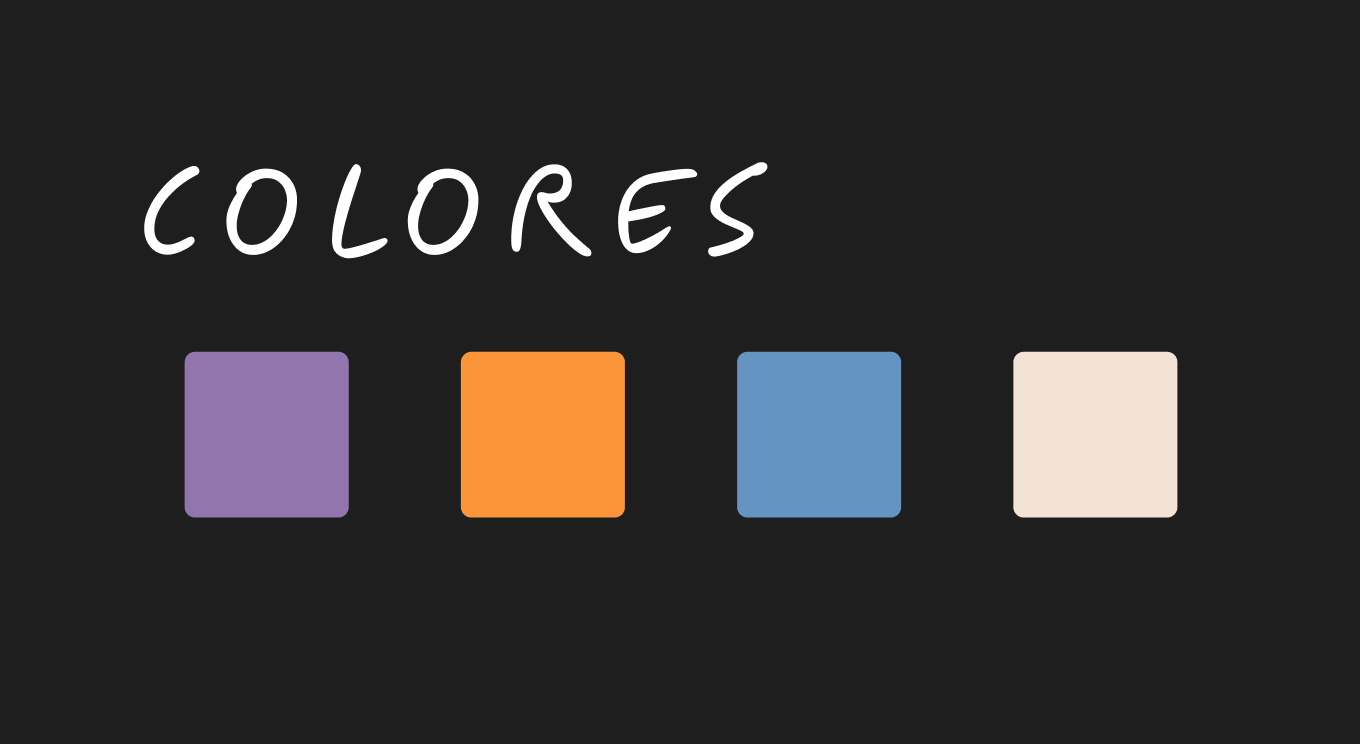
\includegraphics[width=7cm]{Colors.jpg}\par}
		\caption{Paleta}
	\end{center}
\end{figure}

Como fuente, se opta por escoger la fuente \textit{Nunito Sans}, que proporciona Google. Se escoge porque es una fuente bastante estándar y legible para cualquier tipo de usuario.

\begin{figure}[H]
	\begin{center}
		{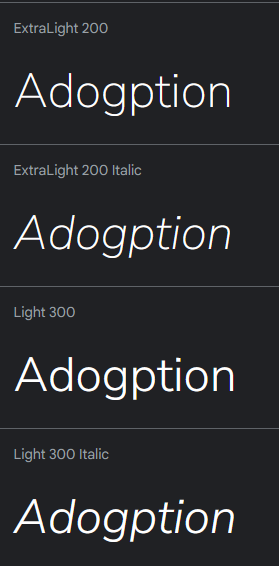
\includegraphics[width=7cm]{NunitoFont.png}\par}
		\caption{Fuente Nunito Sans}
	\end{center}
\end{figure}

\subsubsection{Nombre}

Como nombre de la aplicación,  se tiene en cuenta que inicialmente la aplicación está dirigida a la adopción de perros, así que se propone un juego de palabras. Uniendo las palabras \textit{Adoption} y \textit{Dog}, que son la traducción de las palabras adopción y perro, conformando el nombre: \textbf{\textit{Adogption}}.

\subsubsection{Logo e iconos}

La última parte relacionada con el branding en este proyecto es la de generación de logos e iconos. En esta sección se incluye tanto el logo de la aplicación como los iconos que se han hecho para incluir dentro de la aplicación. Algunos de los iconos podrían finalmente no utilizarse.

La idea del logo es que se perciba claramente que la aplicación va sobre perros. Los corgis son unas de las razas más populares en el mundo, destacan por que es una raza muy amigable y muy querida dentro de la cultura pop, lo que la convierte en la cara perfecta para llamar la atención. Además del logo principal, se ha diseñado un logo animado para incluir en pantallas de carga u otros lugar. Por último, se han hecho algunos iconos por defecto, que serán utilizados en perfiles o listas.


\begin{figure}[H]
   	\begin{subfigure}{0.48\textwidth}
		\begin{center}
			{
\includegraphics[width=6cm]{Logo1.png}\par}
			\caption{Logo}
		\end{center}  
	\end{subfigure}\hfill
   	\begin{subfigure}{0.48\textwidth}
		\begin{center}
			{
\includegraphics[width=7cm]{ADOGPTIONFIXED.png}\par}
			\caption{Logo animado}
		\end{center}  
	\end{subfigure}\hfill
	\caption{Logos}
\end{figure}


\begin{figure}[H]
   	\begin{minipage}{0.48\textwidth}
		\begin{center}
			{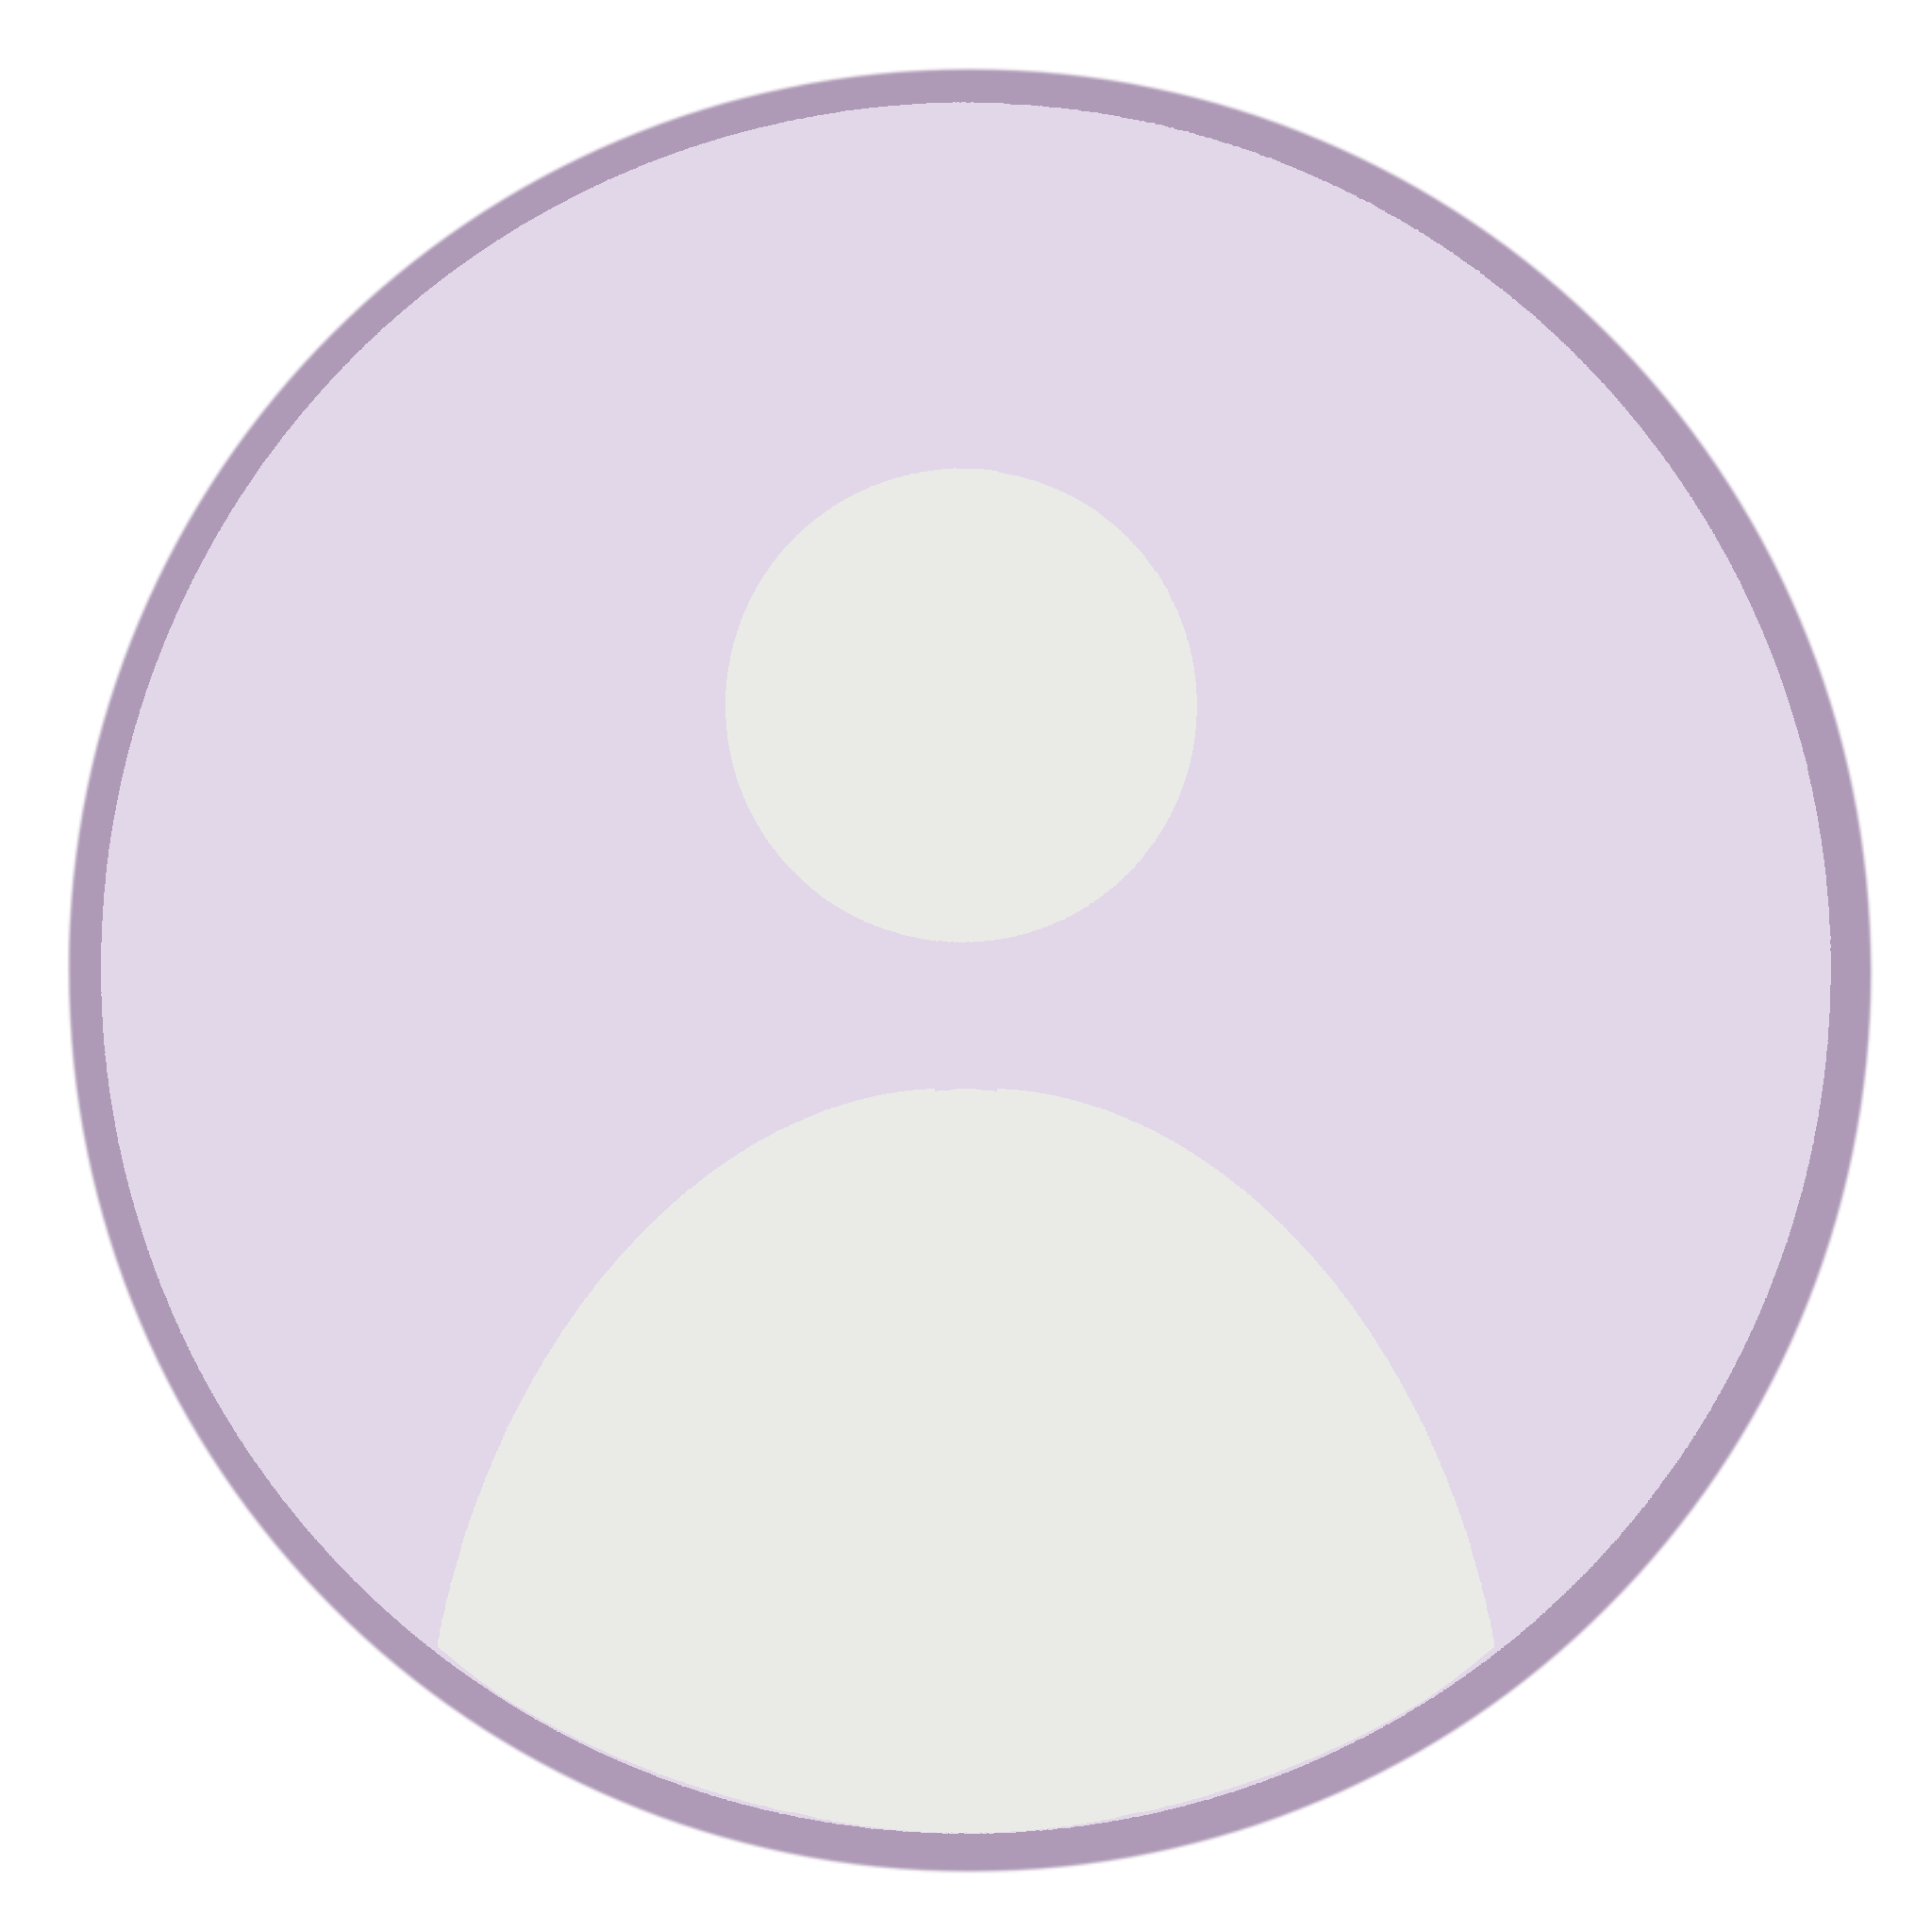
\includegraphics[width=6cm]{EMPTYUSER.png}\par}
			\caption{Icono por defecto para usuario}
		\end{center}  
	\end{minipage}\hfill
   	\begin{minipage}{0.48\textwidth}
		\begin{center}
			{
\includegraphics[width=6cm]{EMPTYDOG.png}\par}
			\caption{Icono por defecto para perro}
		\end{center}  
	\end{minipage}\hfill
\end{figure}


\begin{figure}[H]
   	\begin{minipage}{0.48\textwidth}
		\begin{center}
			{
\includegraphics[width=6cm]{Adoptar.png}\par}
			\caption{Icono para listas de adopción}
		\end{center}  
	\end{minipage}\hfill
   	\begin{minipage}{0.48\textwidth}
		\begin{center}
			{
\includegraphics[width=6cm]{Acoger.png}\par}
			\caption{Icono para listas de acogida}
		\end{center}  
	\end{minipage}\hfill
\end{figure}

\begin{figure}[H]
   	\begin{minipage}{0.48\textwidth}
		\begin{center}
			{
\includegraphics[width=6cm]{USERNV.png}\par}
			\caption{Icono usuario no verificado}
		\end{center}  
	\end{minipage}\hfill
   	\begin{minipage}{0.48\textwidth}
		\begin{center}
			{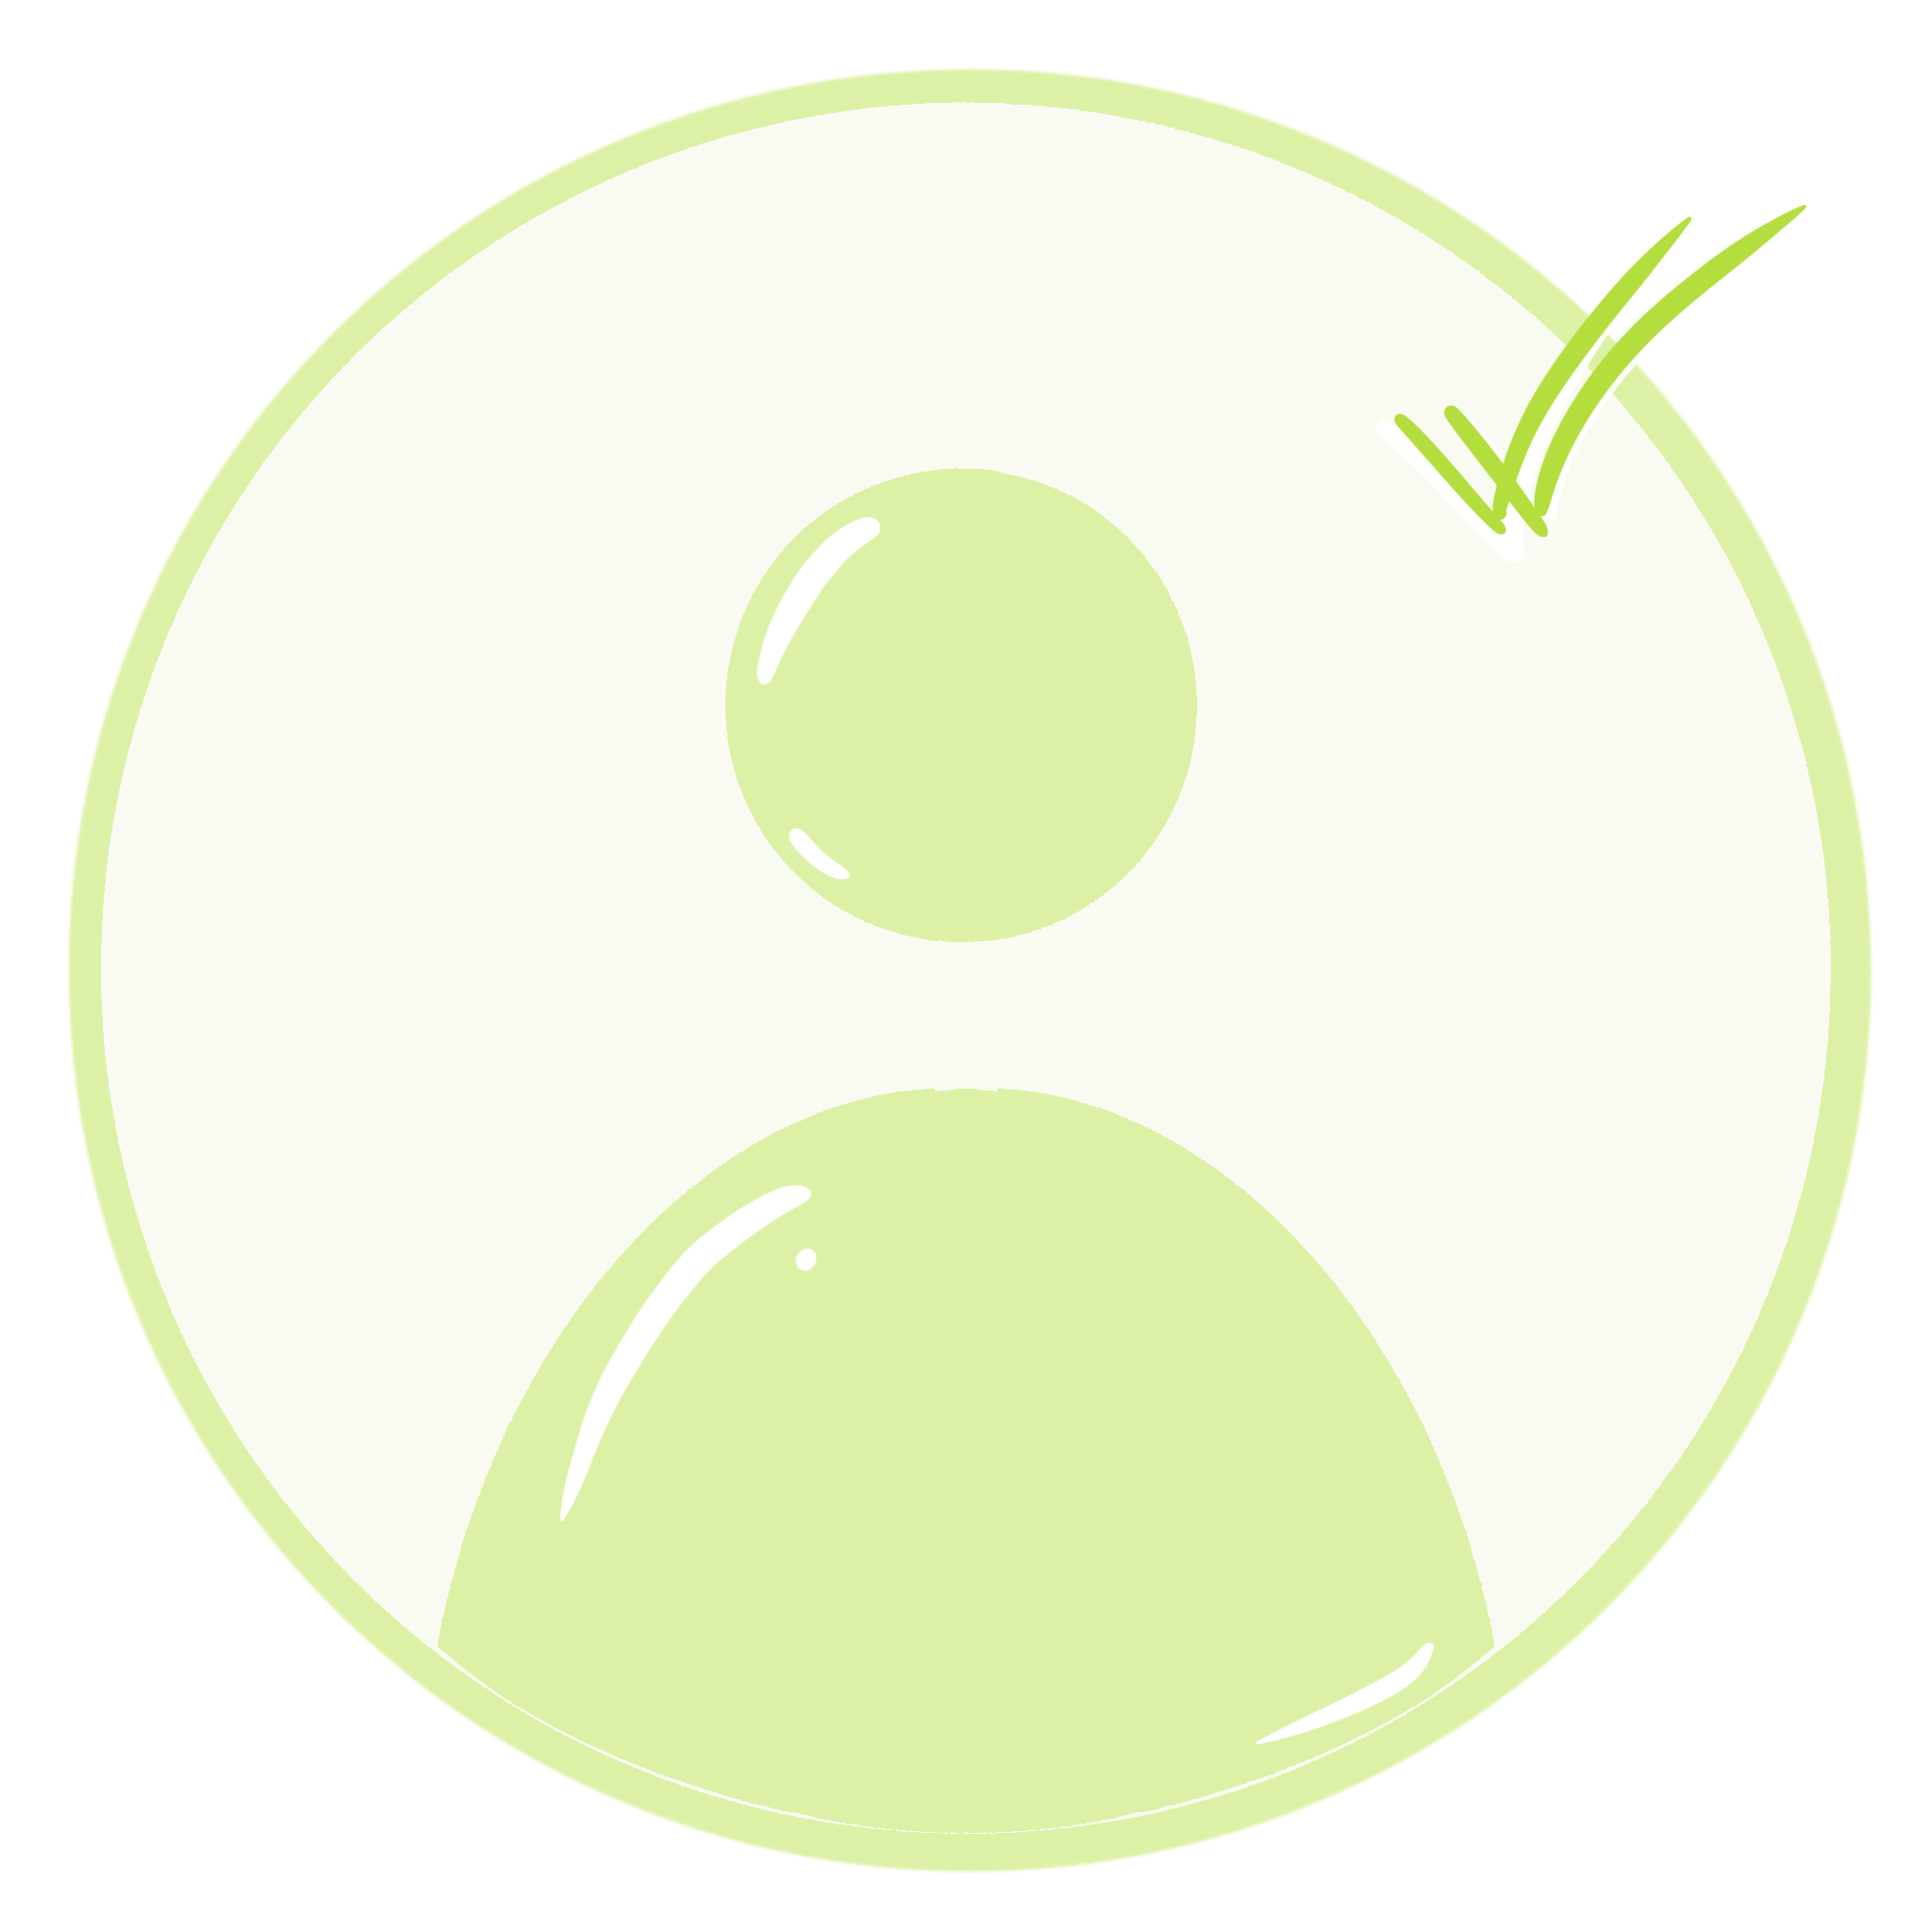
\includegraphics[width=6cm]{USERV.png}\par}
			\caption{Icono usuario verificado}
		\end{center}  
	\end{minipage}\hfill
\end{figure}

\begin{figure}[H]
   	\begin{minipage}{0.48\textwidth}
		\begin{center}
			{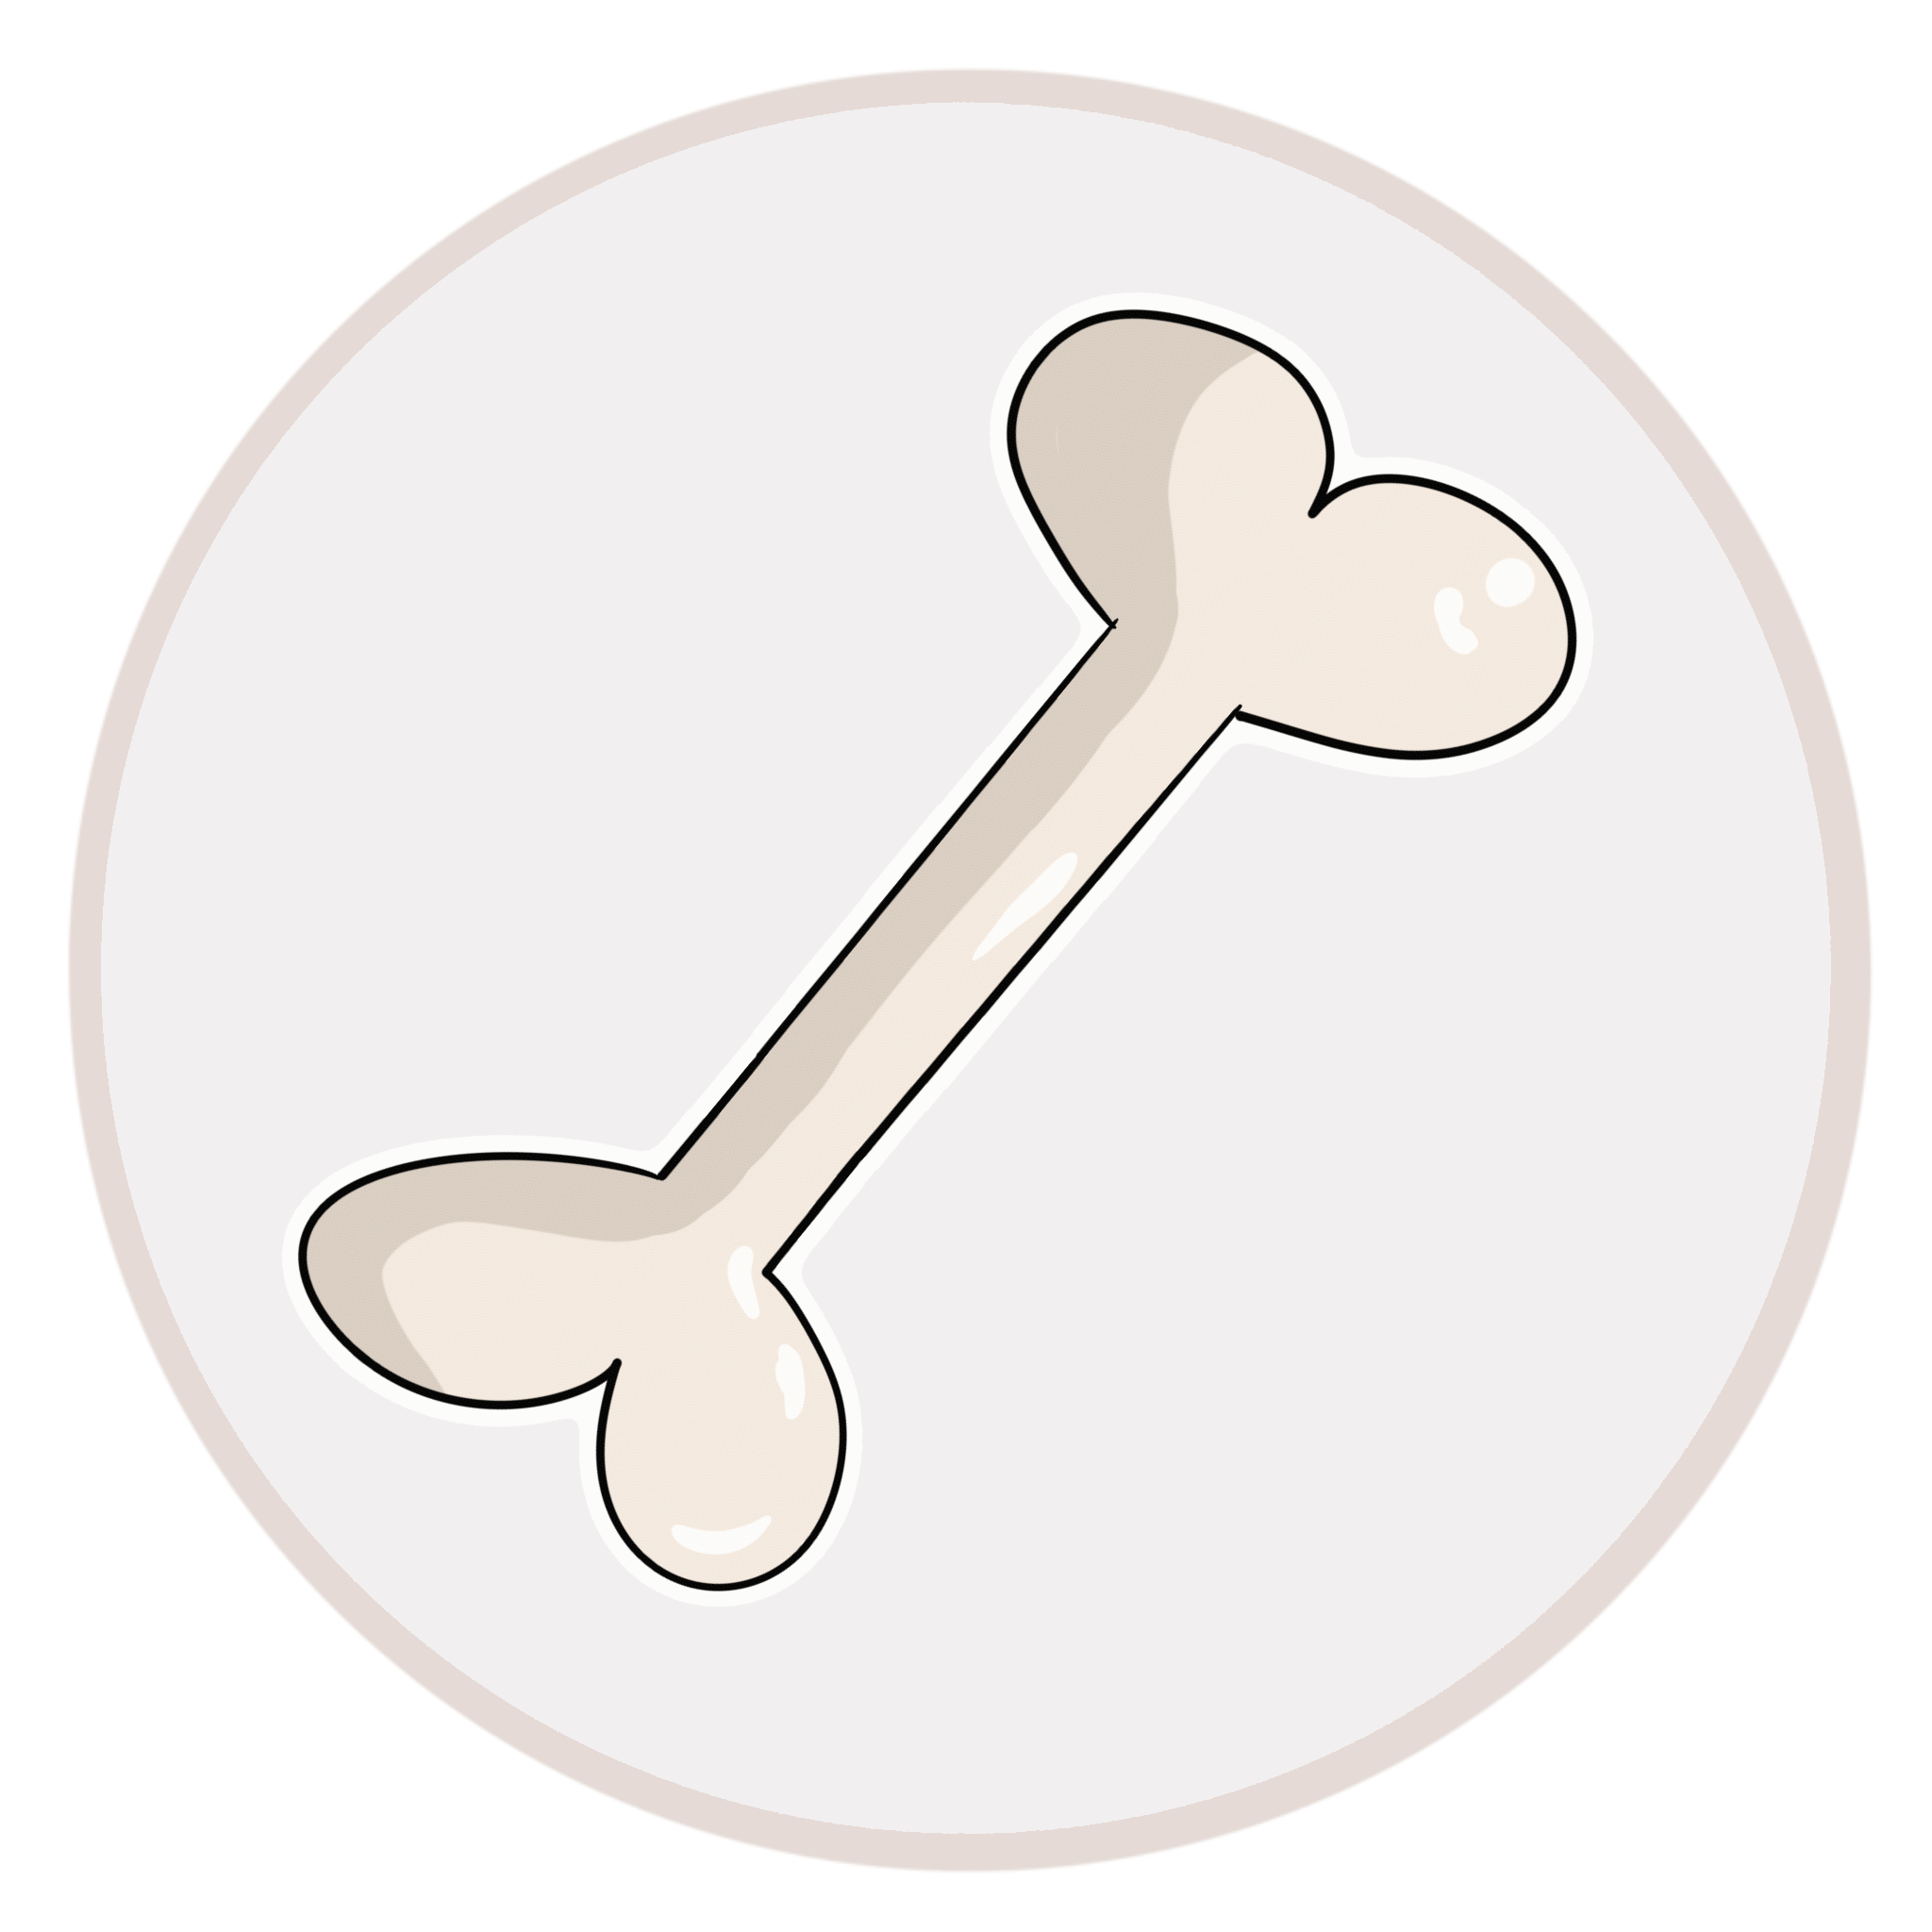
\includegraphics[width=6cm]{Protectora.png}\par}
			\caption{Icono hueso}
		\end{center}  
	\end{minipage}\hfill
   	\begin{minipage}{0.48\textwidth}
		\begin{center}
			{
\includegraphics[width=6cm]{Casa.png}\par}
			\caption{Icono casa}
		\end{center}  
	\end{minipage}\hfill
\end{figure}


\begin{figure}[H]
   	\begin{subfigure}{0.48\textwidth}
		\begin{center}
			{
\includegraphics[width=6cm]{ALLUSER.png}\par}
			\caption{Icono en morado}
		\end{center}  
	\end{subfigure}\hfill
   	\begin{subfigure}{0.48\textwidth}
		\begin{center}
			{
\includegraphics[width=6cm]{USER.png}\par}
			\caption{Icono en azul}
		\end{center}  
	\end{subfigure}\hfill
	\caption{Iconos usuarios}
\end{figure}

\begin{figure}[H]
   	\begin{subfigure}{0.48\textwidth}
		\begin{center}
			{
\includegraphics[width=6cm]{Pata1.png}\par}
			\caption{Icono en naranja}
		\end{center}  
	\end{subfigure}\hfill
   	\begin{subfigure}{0.48\textwidth}
		\begin{center}
			{
\includegraphics[width=6cm]{Pata2.png}\par}
			\caption{Icono en morado}
		\end{center}  
	\end{subfigure}\hfill
   	\begin{subfigure}{0.48\textwidth}
		\begin{center}
			{
\includegraphics[width=6cm]{Pata3.png}\par}
			\caption{Icono en azul}
		\end{center}  
	\end{subfigure}\hfill
	\caption{Iconos patas}
\end{figure}


\newpage
\subsubsection{Diseños}

En esta sección se incluyen todos los diseños realizados en \textit{Miró} para las pantallas de la aplicación. Entre los diseños se encuentran todas las páginas principales de la aplicación y componentes relevantes. En la sección de implementación se especificará la función de cada una de las pantallas.


\begin{figure}[H]
   	\begin{minipage}{0.48\textwidth}
		\begin{center}
			{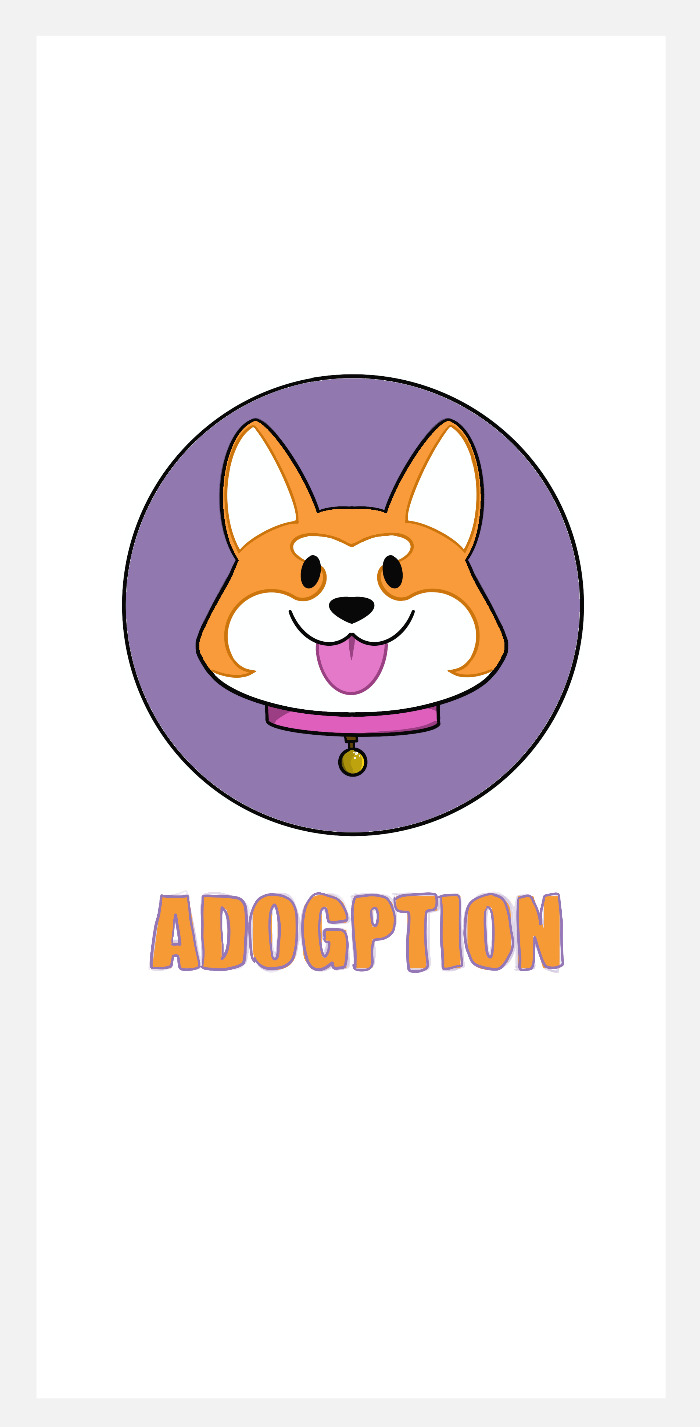
\includegraphics[height=8cm]{SplashScreen.jpg}\par}
			\caption{Pantalla de carga.}
			\medskip
		\end{center}  
	\end{minipage}\hfill
   	\begin{minipage}{0.48\textwidth}
		\begin{center}
			{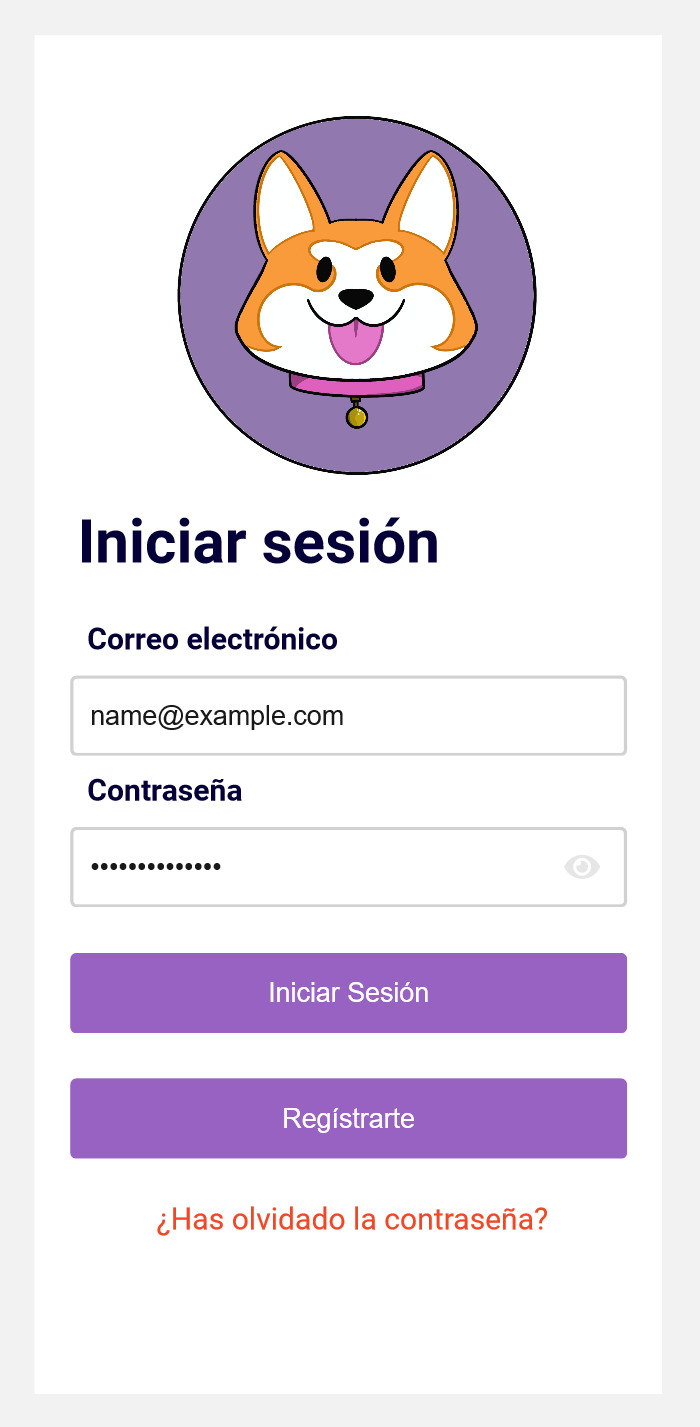
\includegraphics[height=8cm]{Login.jpg}\par}
			\caption{Inicio de sesión.}
			\medskip
		\end{center}  
	\end{minipage}\hfill
\end{figure}


\begin{figure}[H]
   	\begin{minipage}{0.48\textwidth}
		\begin{center}
			{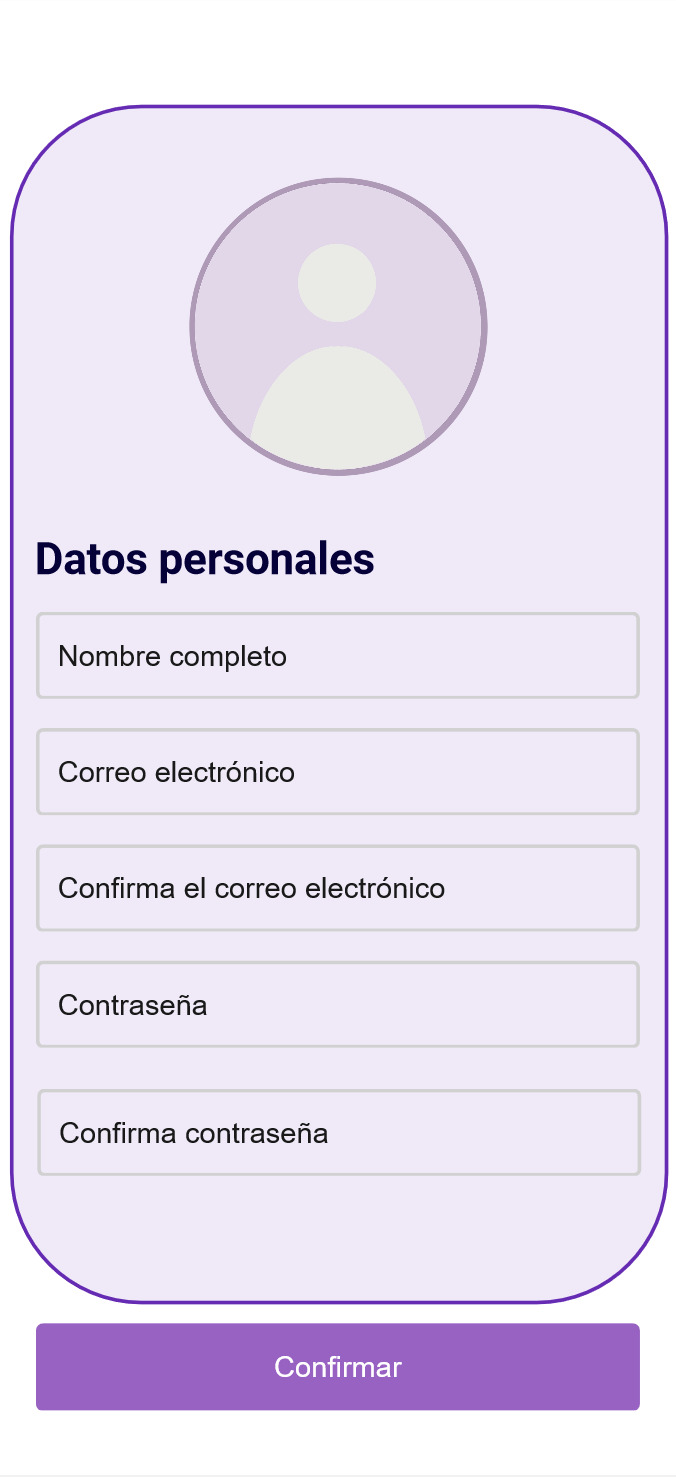
\includegraphics[height=8cm, width=4cm]{UserRegister.jpg}\par}
			\caption{Registro/edición de usuario.}
			\medskip
		\end{center}  
	\end{minipage}\hfill
   	\begin{minipage}{0.48\textwidth}
		\begin{center}
			{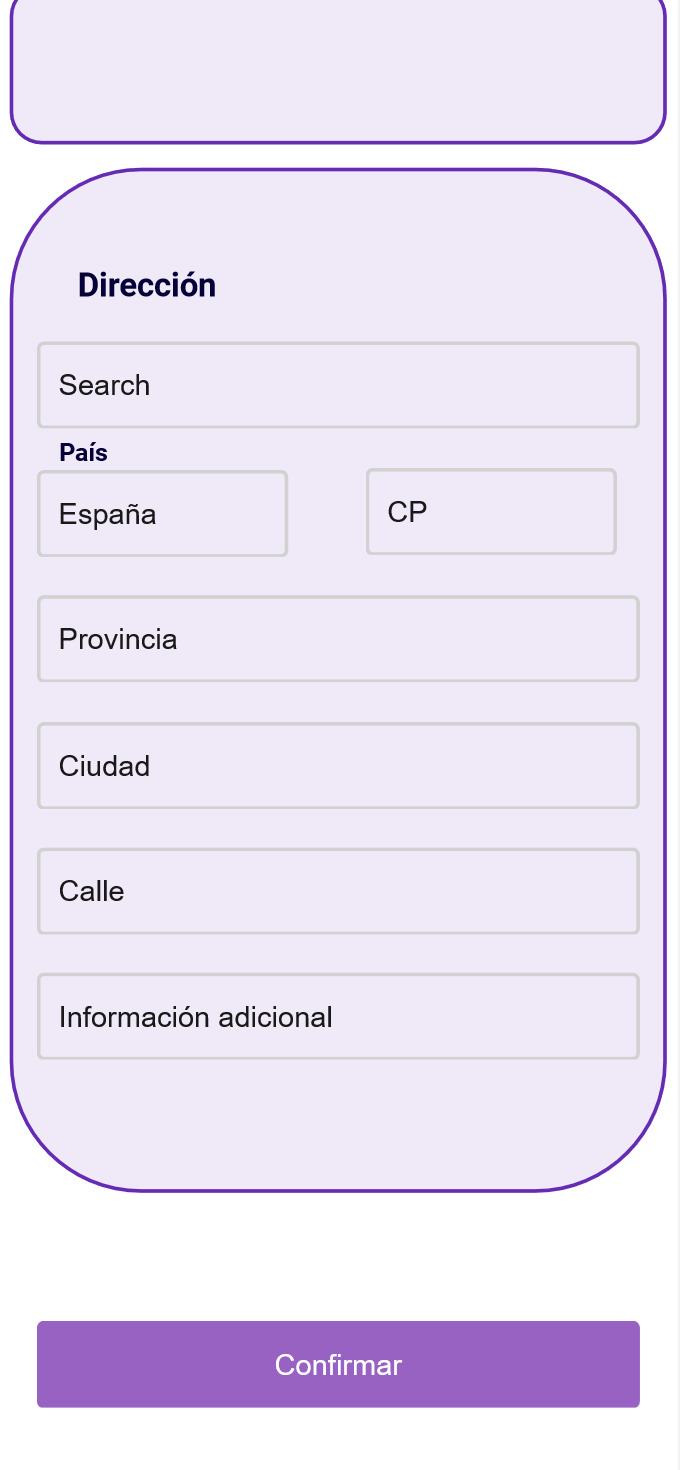
\includegraphics[height=8cm, width=4cm]{CompanyRegister.jpg}\par}
			\caption{Registro/edición de protectora.}
			\medskip
		\end{center}  
	\end{minipage}\hfill
\end{figure}

\begin{figure}[H]
   	\begin{minipage}{0.48\textwidth}
		\begin{center}
			{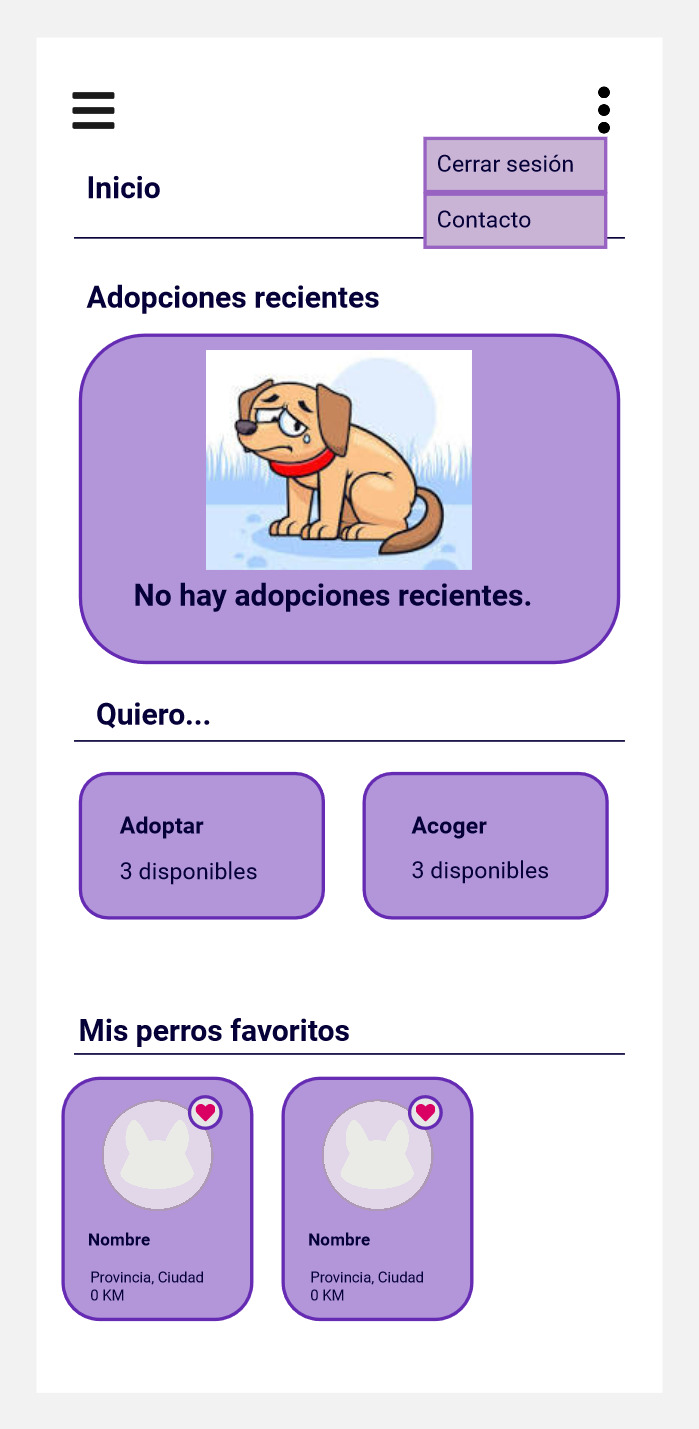
\includegraphics[height=8cm, width=4cm]{UserPage.jpg}\par}
			\caption{Inicio usuario.}
			\medskip
			\small

		\end{center}  
	\end{minipage}\hfill
   	\begin{minipage}{0.48\textwidth}
		\begin{center}
			{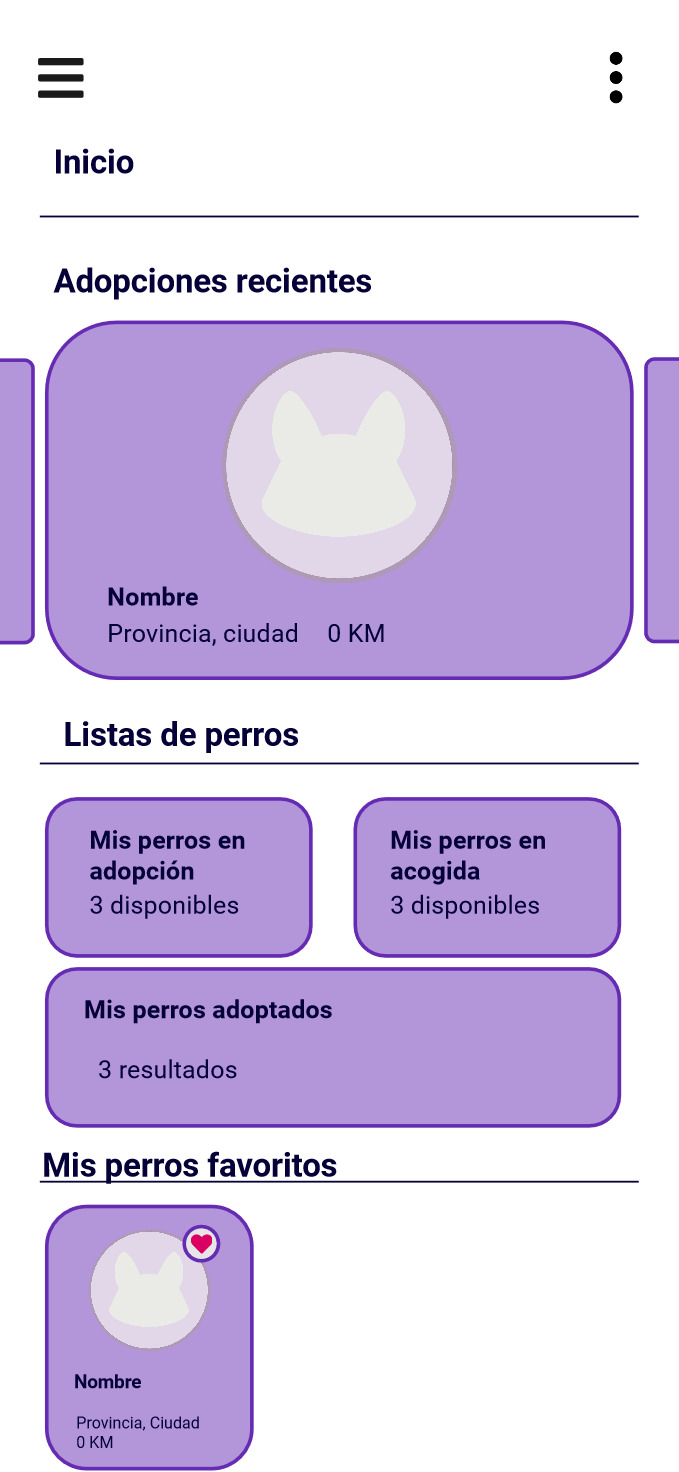
\includegraphics[height=8cm, width=4cm]{CompanyPage.jpg}\par}
			\caption{Inicio protectora.}
			\medskip			
		\end{center}  
	\end{minipage}\hfill
\end{figure}

\begin{figure}[H]
   	\begin{minipage}{0.48\textwidth}
		\begin{center}
			{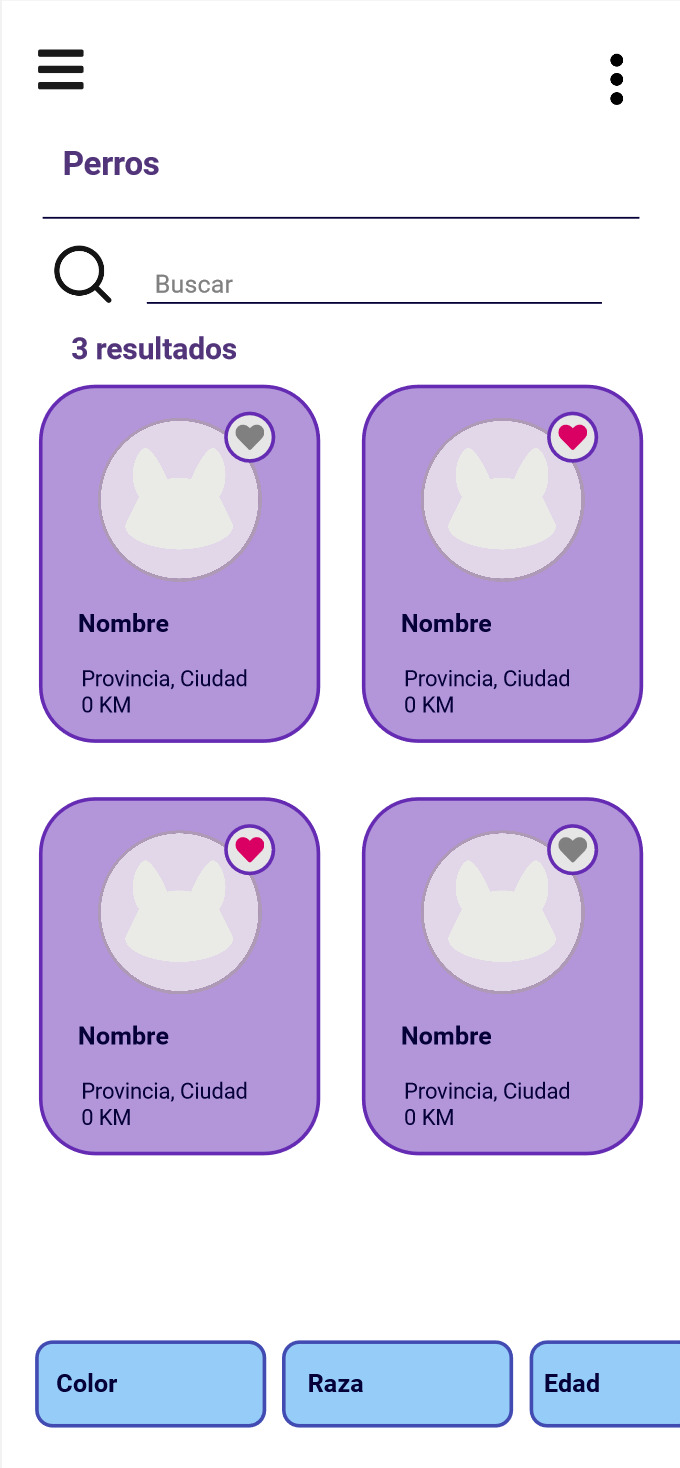
\includegraphics[height=8cm, width=4cm]{DogList.jpg}\par}
			\caption{Lista de perros.}
			\medskip
		\end{center}  
	\end{minipage}\hfill
   	\begin{minipage}{0.48\textwidth}
		\begin{center}
			{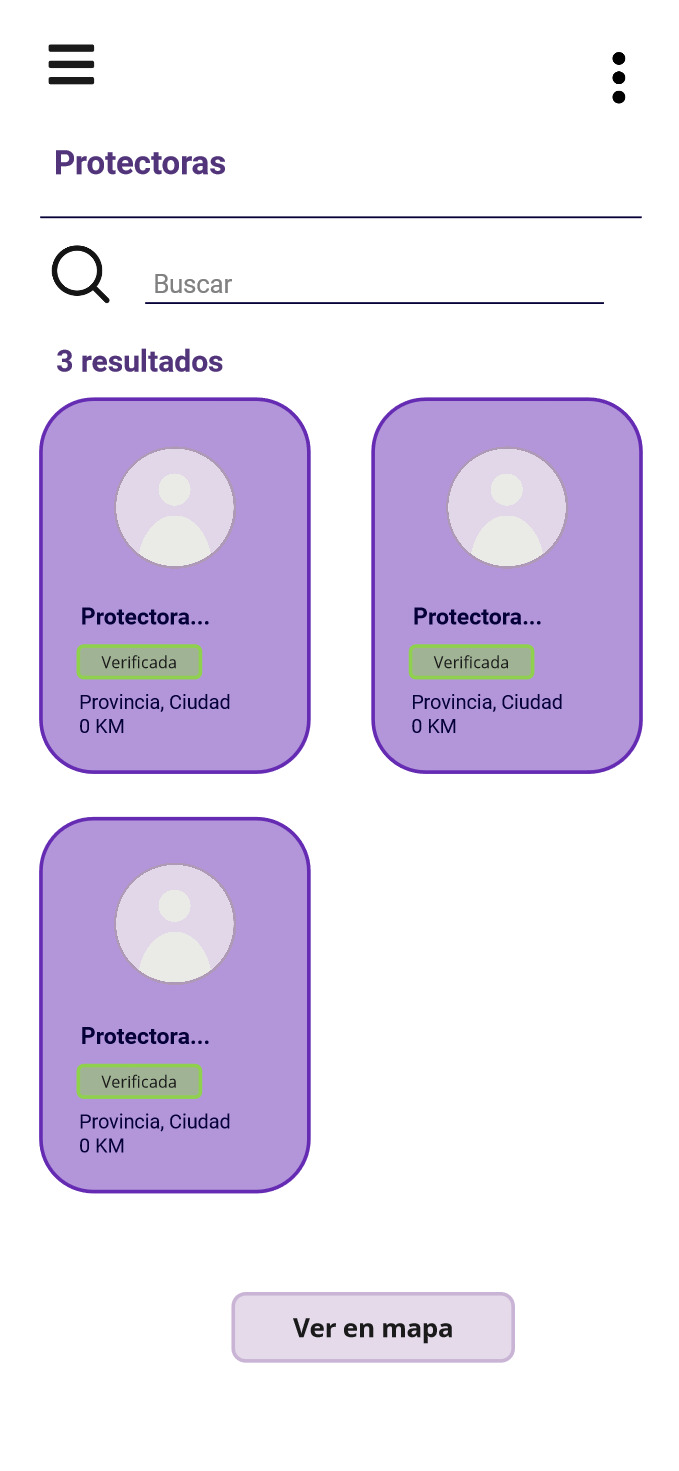
\includegraphics[height=8cm, width=4cm]{UserList.jpg}\par}
			\caption{Lista de usuarios.}
			\medskip
		\end{center}  
	\end{minipage}\hfill
\end{figure}


\begin{figure}[H]
   	\begin{minipage}{0.48\textwidth}
		\begin{center}
			{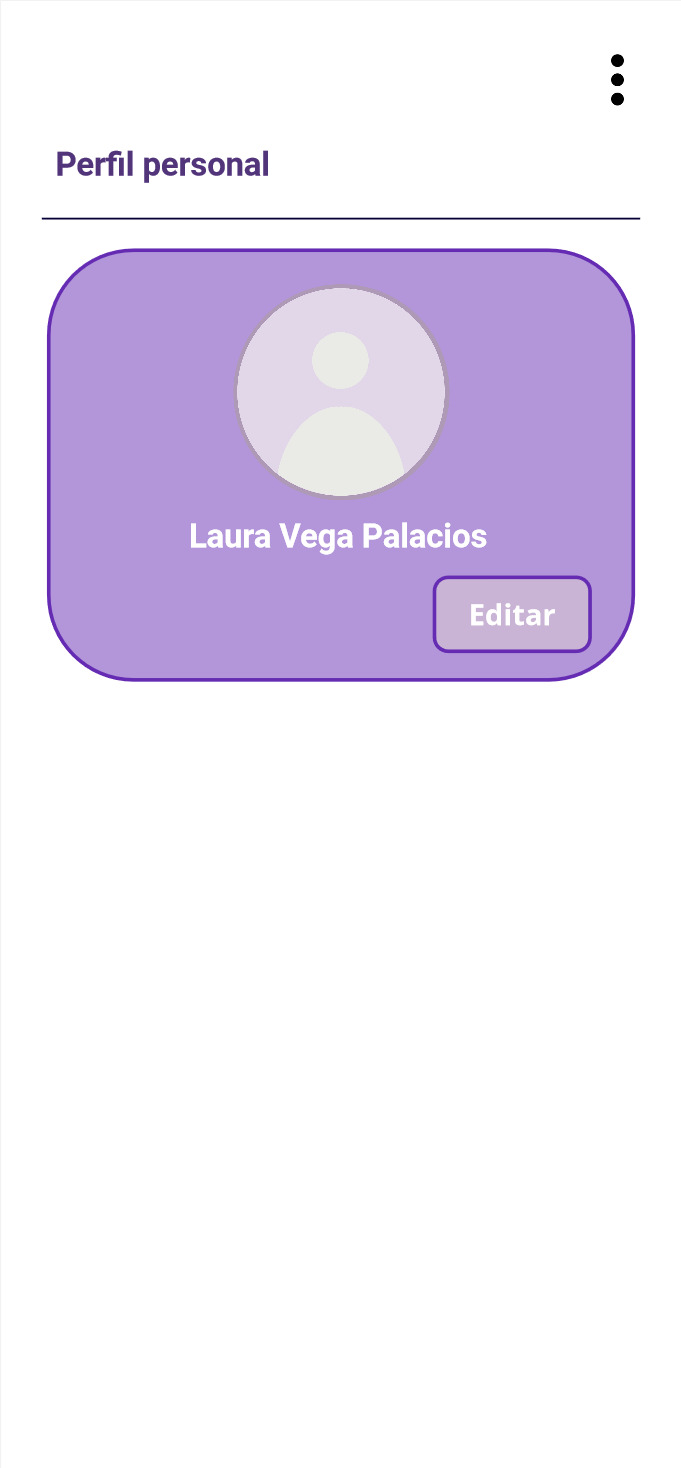
\includegraphics[height=8cm, width=4cm]{UserProfile.jpg}\par}
			\caption{Perfil de usuario/administrador.}
			\medskip

		\end{center}  
	\end{minipage}\hfill
   	\begin{minipage}{0.48\textwidth}
		\begin{center}
			{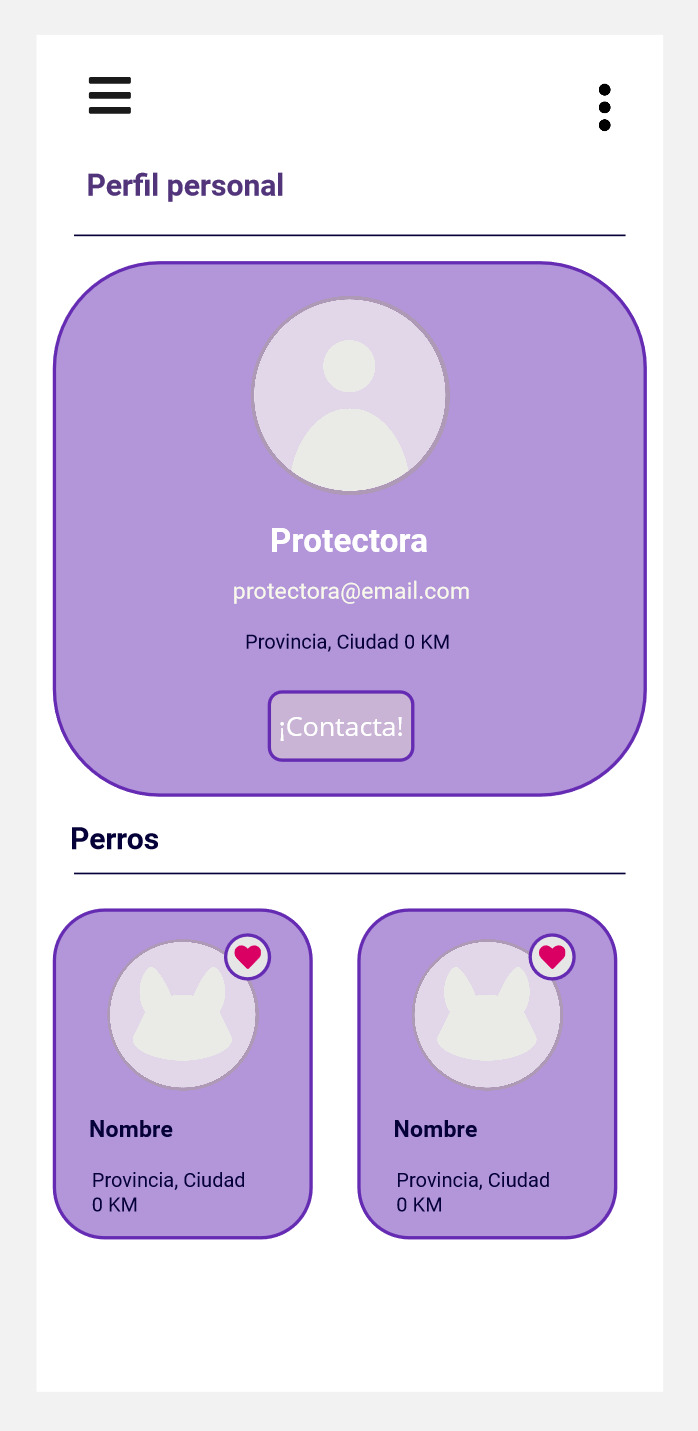
\includegraphics[height=8cm, width=4cm]{CompanyProfile.jpg}\par}
			\caption{Perfil de protectora. }
			\medskip
		\end{center}  
	\end{minipage}\hfill
\end{figure}

\begin{figure}[H]
   	\begin{minipage}{0.48\textwidth}
		\begin{center}
			{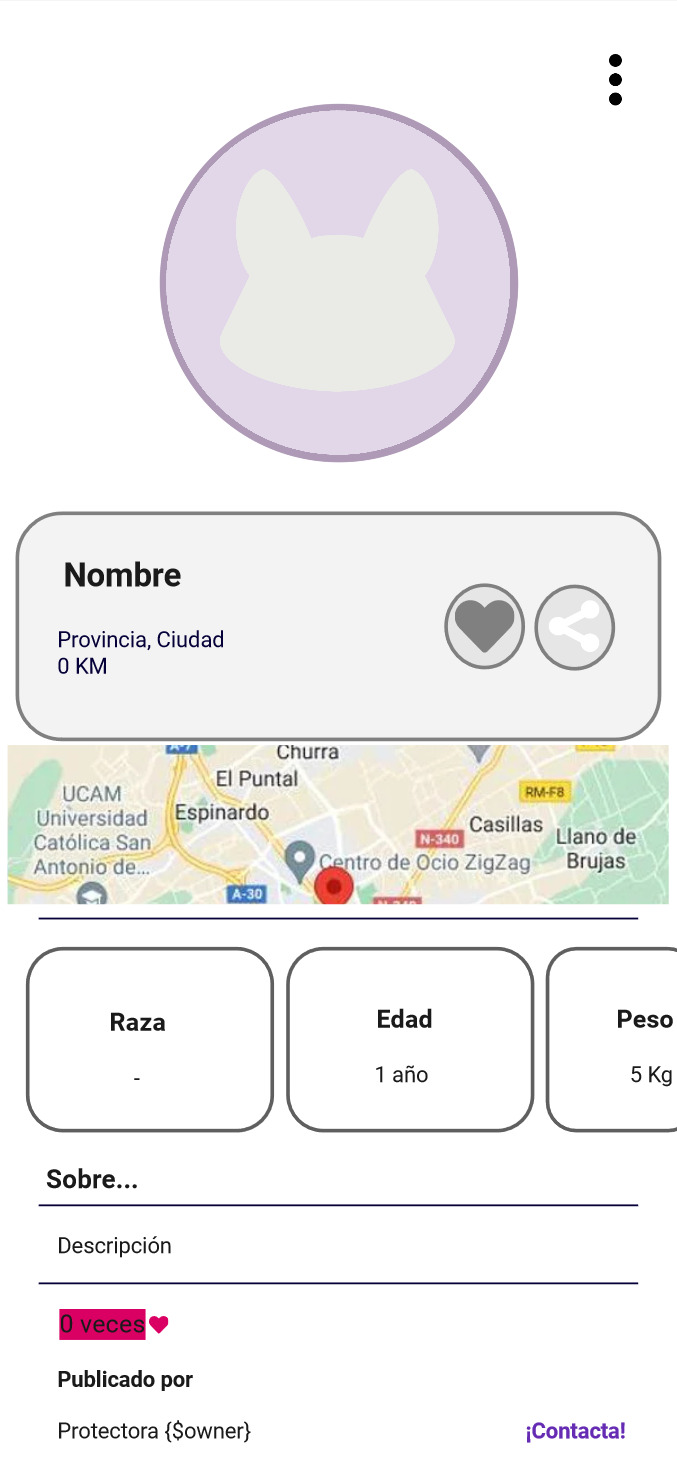
\includegraphics[height=8cm, width=4cm]{DogProfile.jpg}\par}
			\caption{Perfil de perro.}
			\medskip
		\end{center}  
	\end{minipage}\hfill
   	\begin{minipage}{0.48\textwidth}
		\begin{center}
			{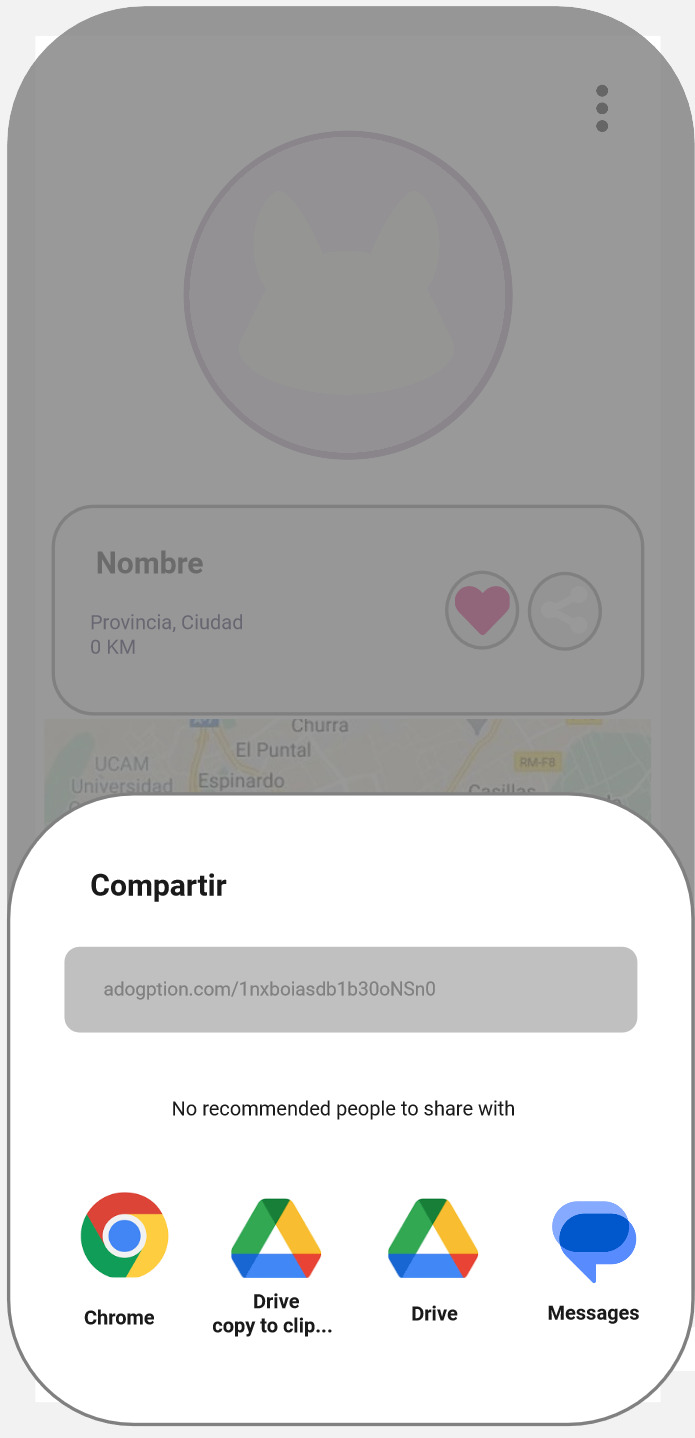
\includegraphics[height=8cm, width=4cm]{ShareAction.jpg}\par}
			\caption{Compartir perro.}
			\medskip
		\end{center}  
	\end{minipage}\hfill
\end{figure}

\begin{figure}[H]
   	\begin{minipage}{0.48\textwidth}
		\begin{center}
			{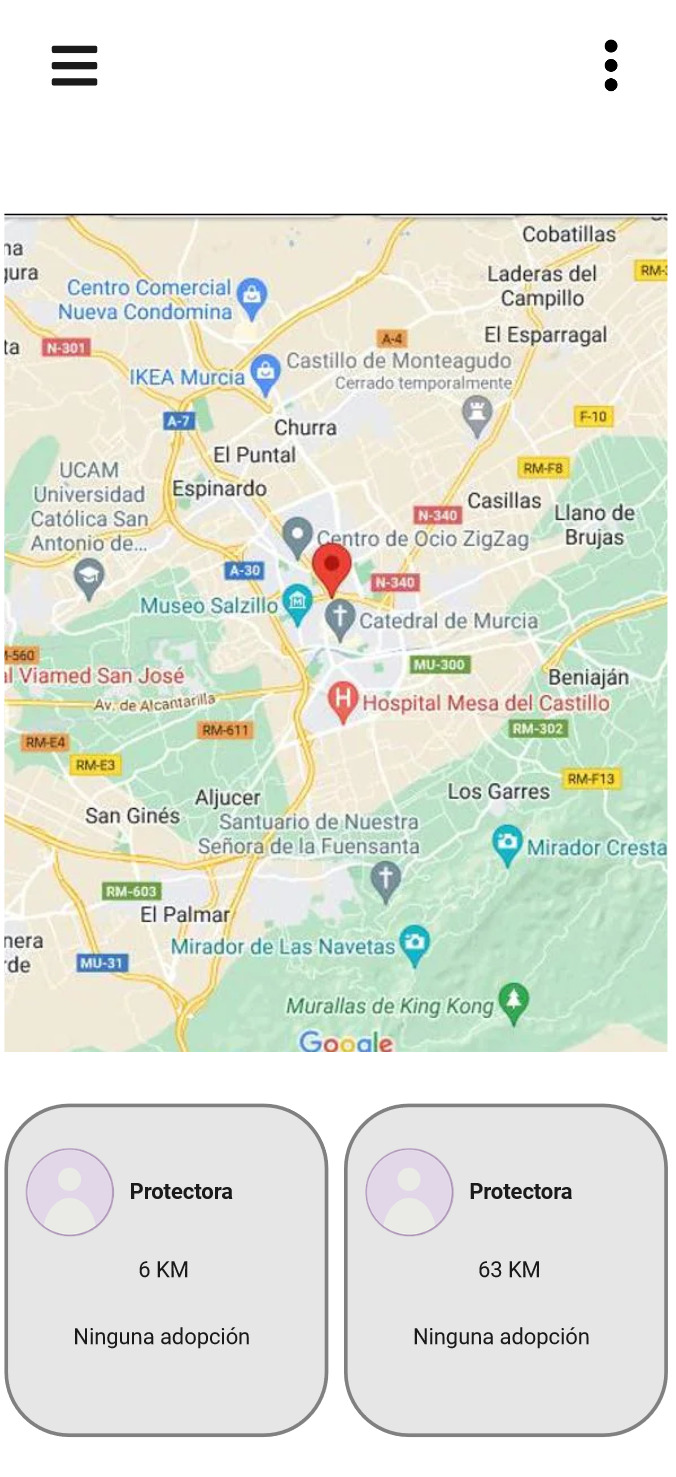
\includegraphics[height=8cm, width=4cm]{MapPage.jpg}\par}
			\caption{Página de mapa y lista.}
			\medskip
		\end{center}  
	\end{minipage}\hfill
   	\begin{minipage}{0.48\textwidth}
		\begin{center}
			{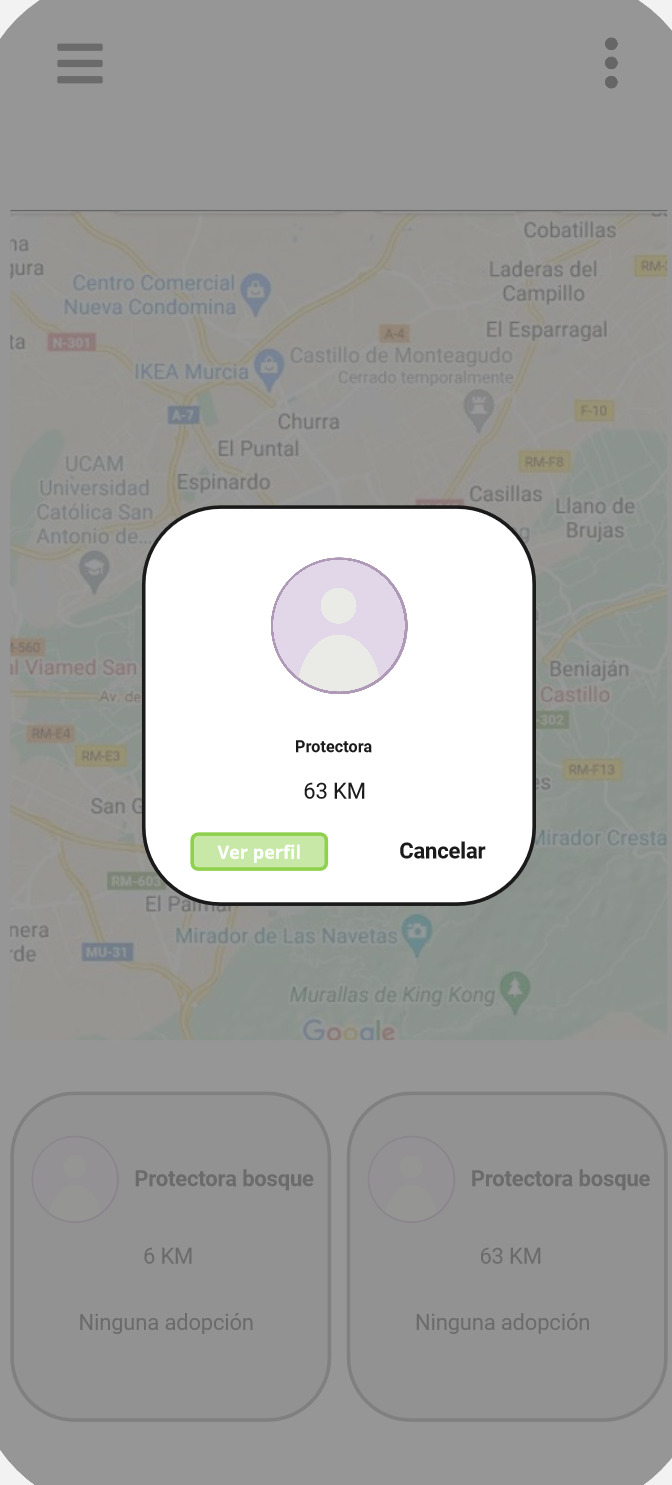
\includegraphics[height=8cm, width=4cm]{MapAction.jpg}\par}
			\caption{Acción de redirigir a perfil.}
			\medskip
		\end{center}  
	\end{minipage}\hfill
\end{figure}

\begin{figure}[H]
   	\begin{minipage}{0.48\textwidth}
		\begin{center}
			{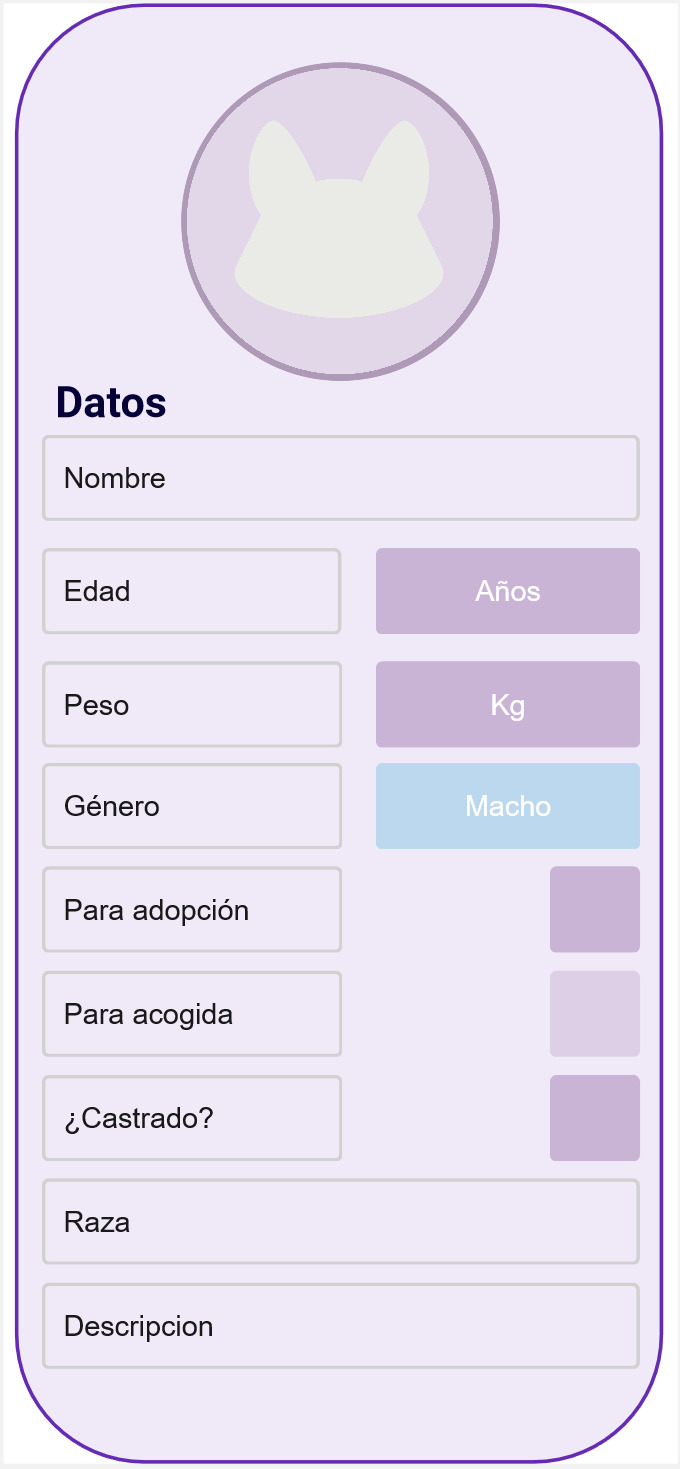
\includegraphics[height=8cm, width=4cm]{RegisterDog.jpg}\par}
			\caption{Registro/edición canino.}
			\medskip
		\end{center}  
	\end{minipage}\hfill
   	\begin{minipage}{0.48\textwidth}
		\begin{center}
			{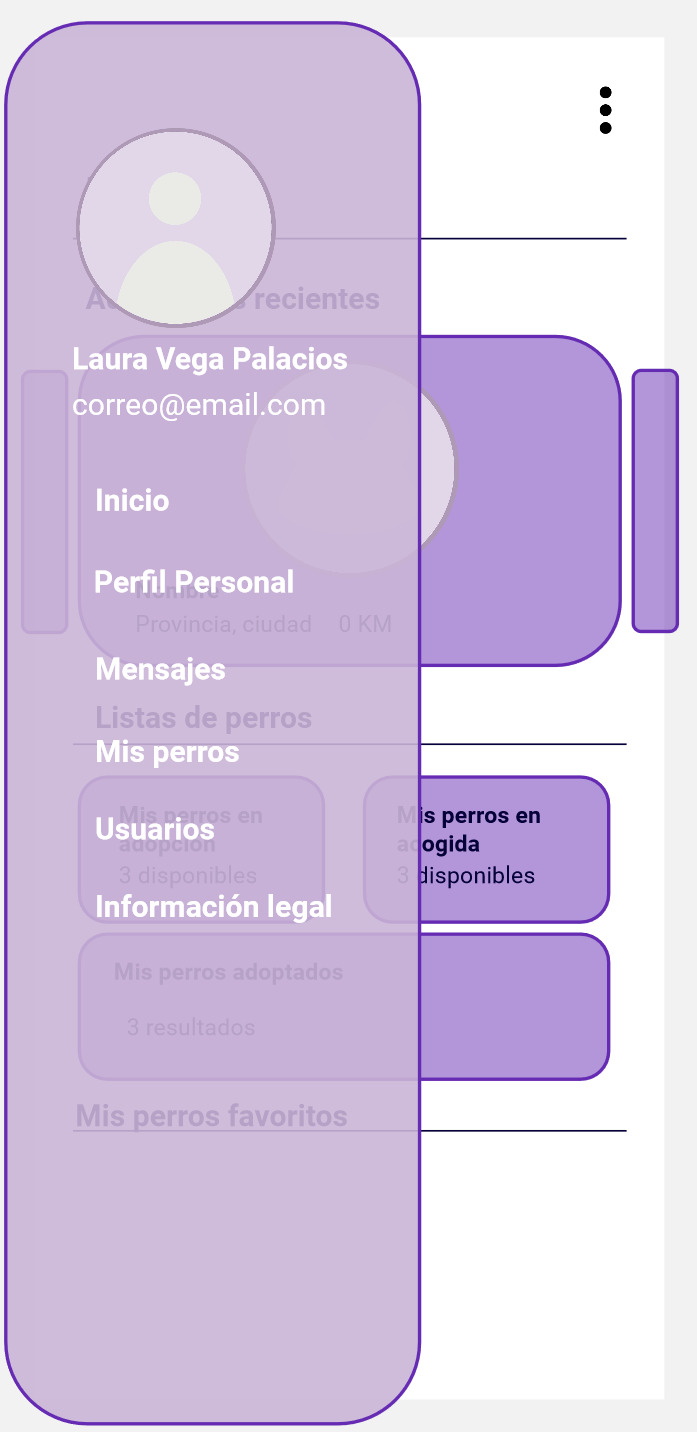
\includegraphics[height=8cm, width=4cm]{SideMenu.jpg}\par}
			\caption{Menú lateral.}
			\medskip
		\end{center}  
	\end{minipage}\hfill
\end{figure}

\begin{figure}[H]
   	\begin{minipage}{0.48\textwidth}
		\begin{center}
			{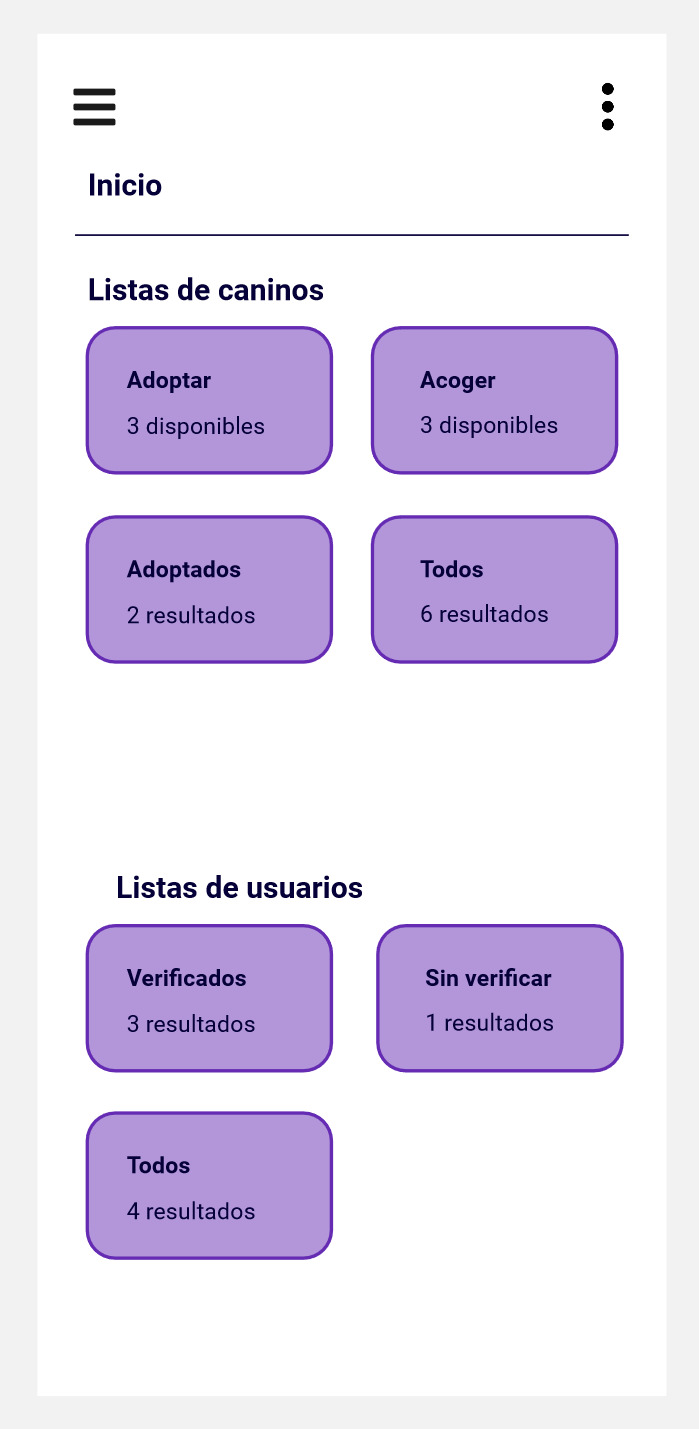
\includegraphics[height=8cm, width=4cm]{AdminPage.jpg}\par}
			\caption{Inicio administrador.}
			\medskip
		\end{center}  
	\end{minipage}\hfill
   	\begin{minipage}{0.48\textwidth}
		\begin{center}
			{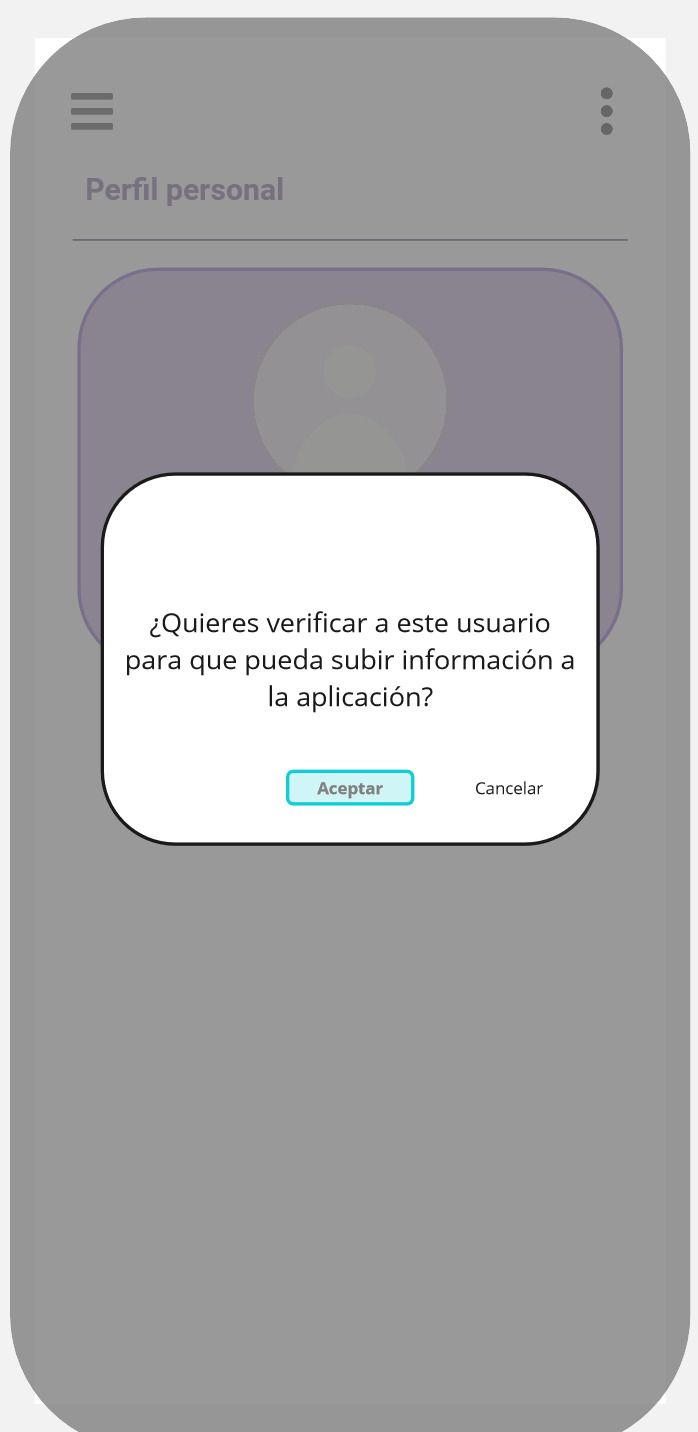
\includegraphics[height=8cm, width=4cm]{VerifyAction.jpg}\par}
			\caption{Pop-up verificación.}
			\medskip
		\end{center}  
	\end{minipage}\hfill
\end{figure}

\begin{figure}[H]
   	\begin{minipage}{0.48\textwidth}
		\begin{center}
			{
\includegraphics[height=8cm, width=4cm]{Notification.jpg}\par}
			\caption{Notificaciones.}
			\medskip
		\end{center}  
	\end{minipage}\hfill
   	\begin{minipage}{0.48\textwidth}
		\begin{center}
			{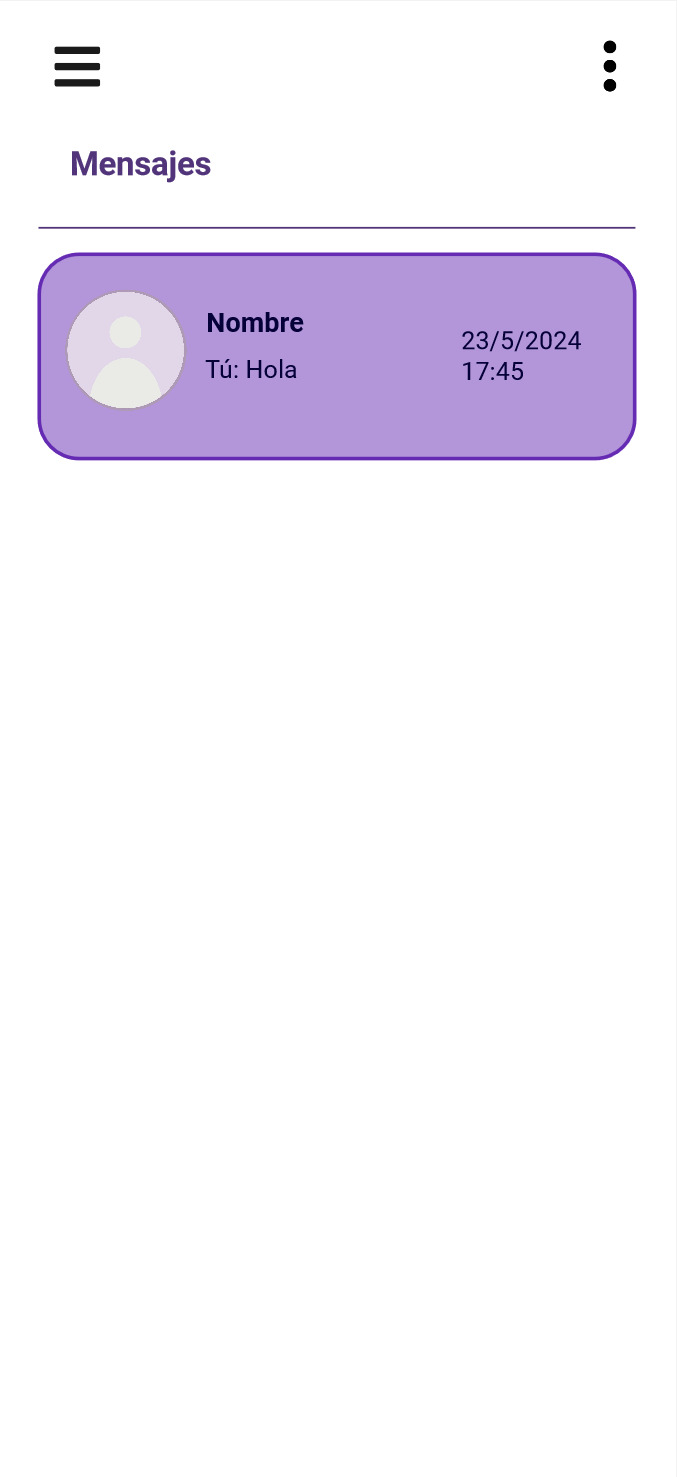
\includegraphics[height=8cm, width=4cm]{Messages.jpg}\par}
			\caption{Página de mensajes.}
			\medskip
		\end{center}  
	\end{minipage}\hfill
\end{figure}

\begin{figure}[H]
   	\begin{minipage}{0.48\textwidth}
		\begin{center}
			{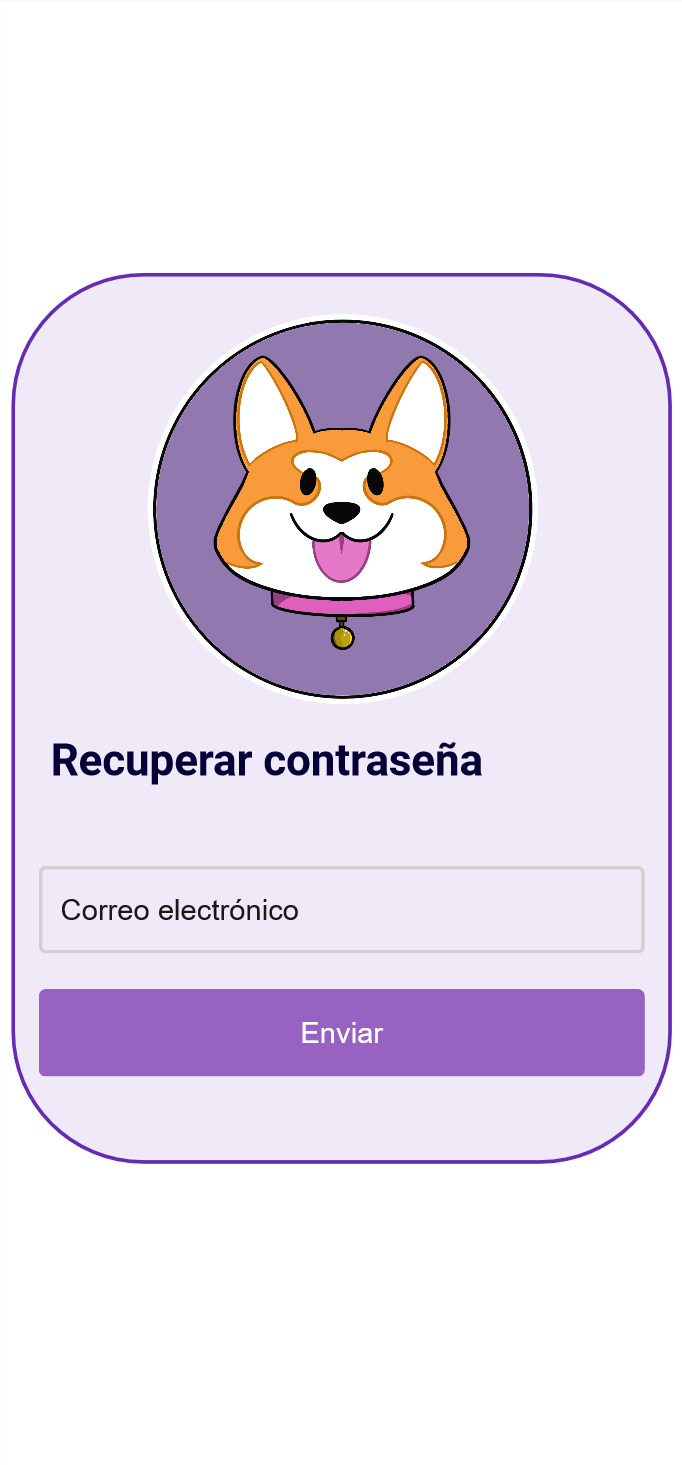
\includegraphics[height=8cm, width=4cm]{PasswordRecovery.jpg}\par}
			\caption{Recuperar contraseña.}
			\medskip
		\end{center}  
	\end{minipage}\hfill
\end{figure}


% Implementación
\newpage
\section{Implementación}

En esta fase se lleva a cabo el desarrollo e implementación de la aplicació. Durante esta etapa, se van completando los diferentes requisitos definidos anteriormente.  Posterior al desarrollo, se realizan pruebas para detectar fallos o faltas de funcionalidades requeridas y, si es necesario, se realizan correcciones.

Durante el desarrollo se han implementado diferentes módulos, cada uno con una finalidad específica:
\begin{itemize}[noitemsep]
	\item \textit{appbar}: contiene una clase encargada de proveer las diferentes app bars que se utilizan en la aplicación.
	\item \textit{auth:} este módulo maneja todas las peticiones que van dirigidas o provieenen del servicio de autenticación de Firebase.
	\item \textit{chats}: incluye todas las clases principales relacionadas con el sistema de mensajería, así como los modelos de los chats.
	\item \textit{common}:
	\item \textit{company}:
	\item \textit{condition}:
	\item \textit{contact}:
	\item \textit{db}: este módulo es uno de los más importantes de la aplicación ya que contiene todas las clases encargadas de gestionar las peticiones con las bases de datos para todas las entidades.
	\item \textit{dog}:
	\item \textit{drawer}:
	\item \textit{home}:
	\item \textit{init}:
	\item \textit{legal}:
	\item \textit{login}:
	\item \textit{message}:
	\item \textit{orderby}:
	\item \textit{register}:
	\item \textit{section}:
	\item \textit{services}:
	\item \textit{splashscreen}:
	\item \textit{update}:
	\item \textit{user}:
	\item \textit{welcome}:
	\item \textit{widget}:
\end{itemize}

Para profundizar en como se ha realizado el desarrollo de la aplicación, se exponen a continuación todas las pantallas con las clases y servicios más importantes involucrados en su implementación.

%Splashscreen
\begin{figure}[H]
	\begin{center}
		{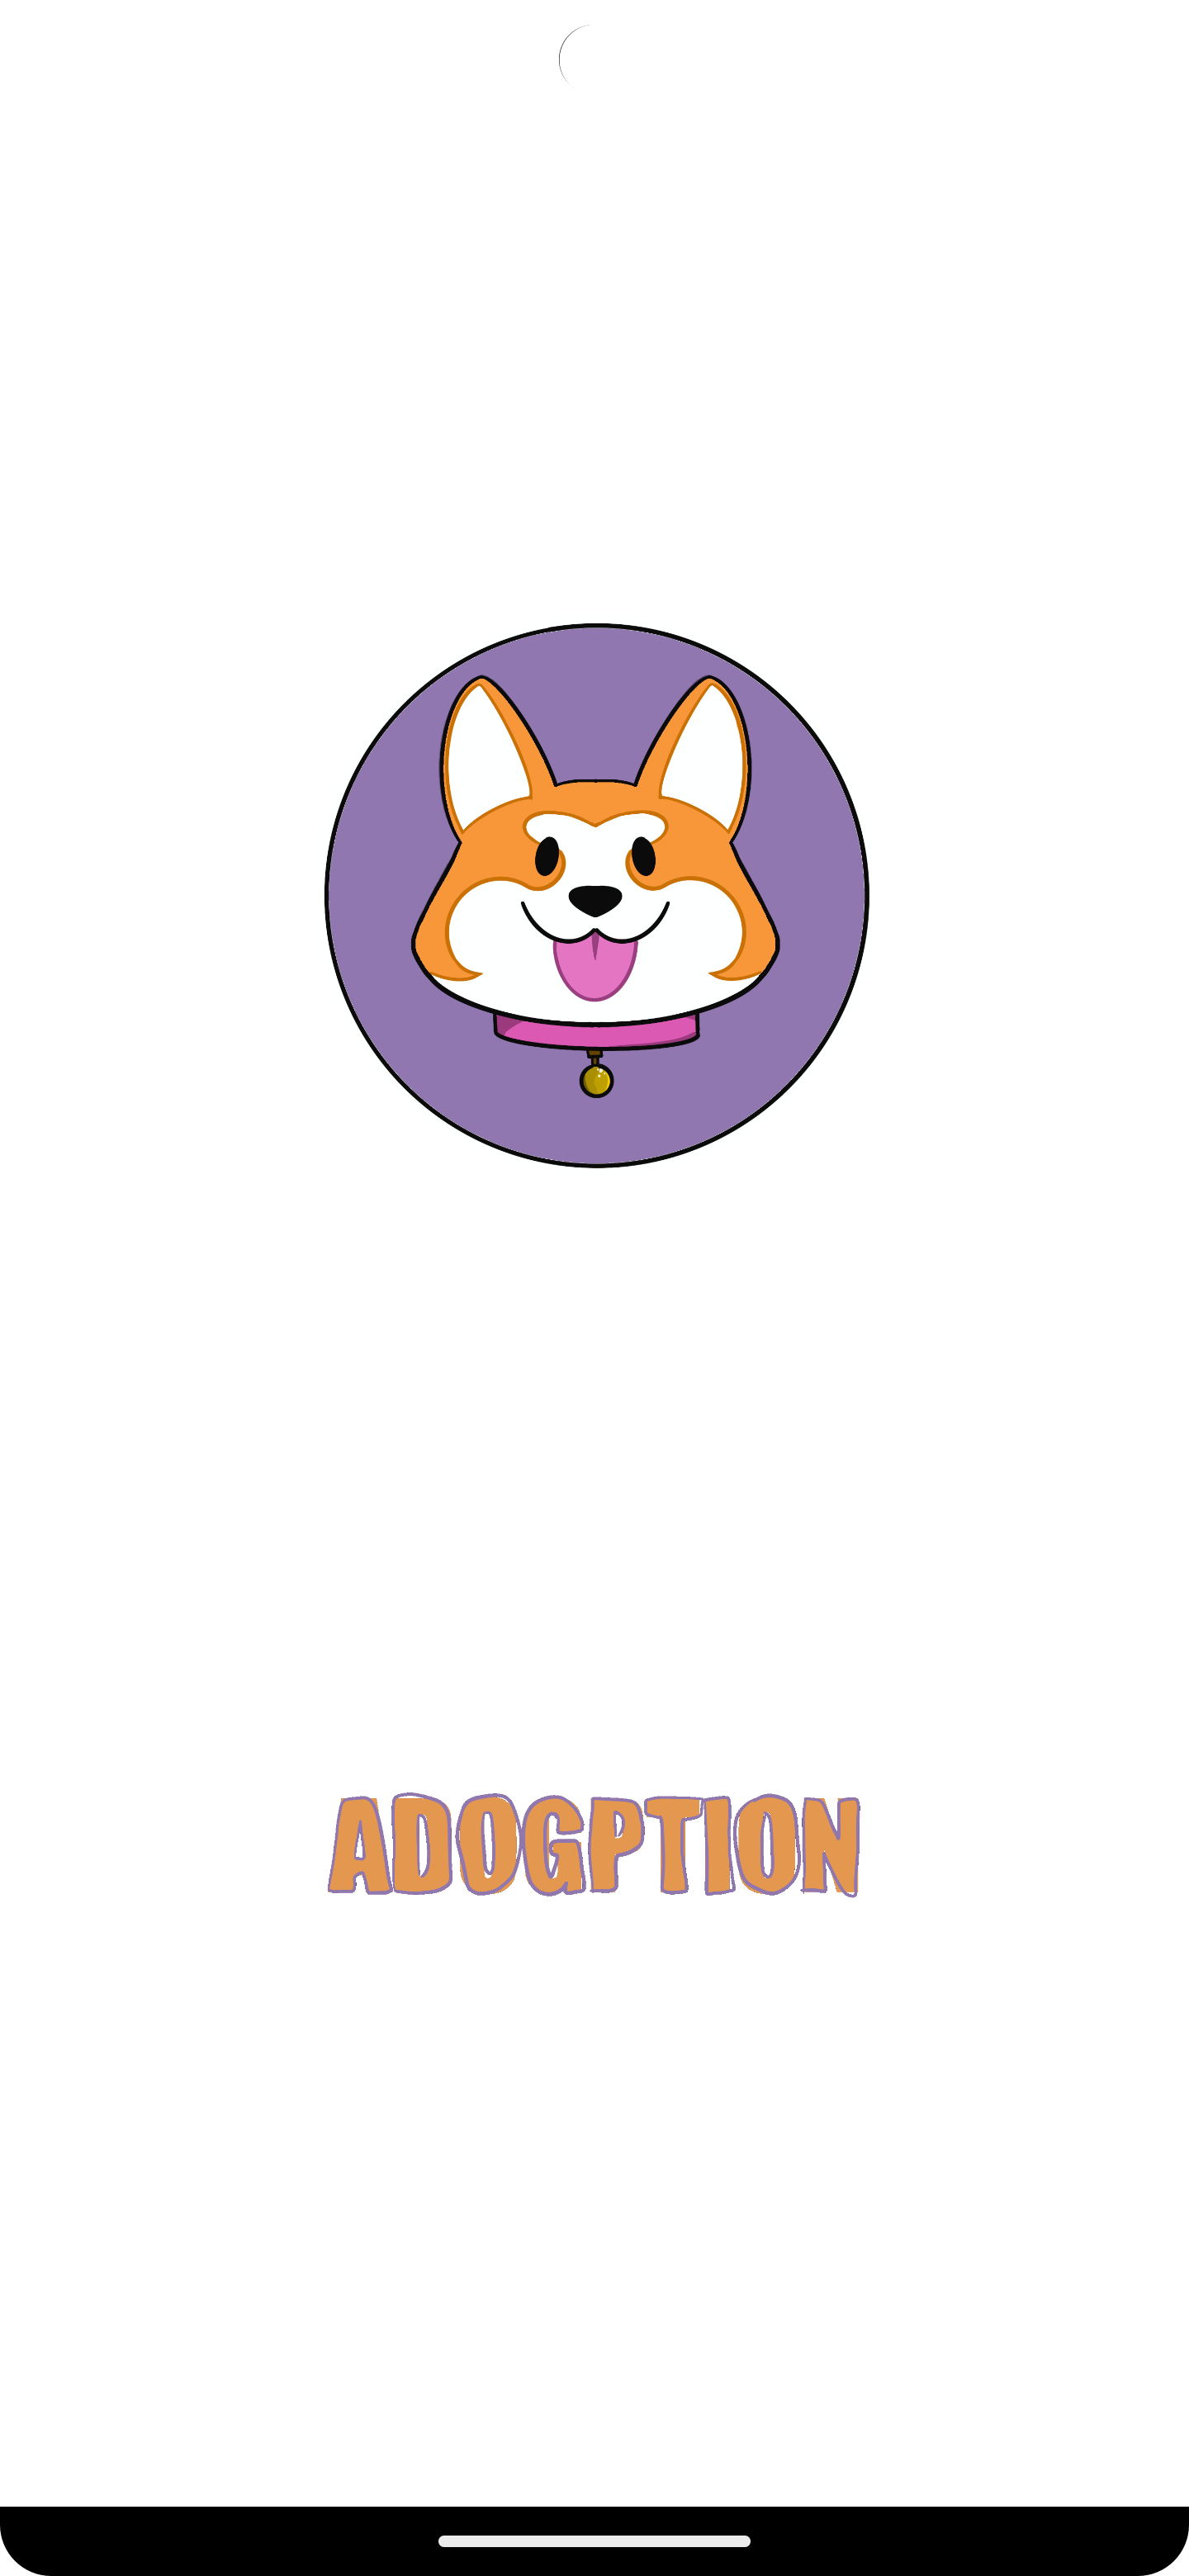
\includegraphics[width=6cm]{app/Splashscreen.png}\par}
		\caption{Página de carga}
	\end{center}
\end{figure}

%Login
\begin{figure}[H]
	\begin{center}
		{\includegraphics[width=6cm]{app/Login.png}\par}
		\caption{Página de inicio de sesión}
	\end{center}
\end{figure}



%Páginas de registro
\begin{figure}[H]
	\begin{center}
		{\includegraphics[width=6cm]{app/Login.png}\par}
		\caption{Página de inicio de sesión}
	\end{center}
\end{figure}


% Vista administrador
\begin{figure}[H]
	\begin{center}
		{\includegraphics[width=6cm]{app/AdminHome.png}\par}
		\caption{Página inicio administrador}
	\end{center}
\end{figure}

\begin{figure}[H]
	\begin{center}
		{\includegraphics[width=6cm]{app/AdminDrawer.png}\par}
		\caption{Menú lateral}
	\end{center}
\end{figure}

\begin{figure}[H]
	\begin{center}
		{\includegraphics[width=6cm]{app/AdminVerifyPopUp}\par}
		\caption{Pop up verificar}
	\end{center}
\end{figure}

\begin{figure}[H]
	\begin{center}
		{\includegraphics[width=6cm]{app/AdminUnVerifyPopUp}\par}
		\caption{Pop up desverificar}
	\end{center}
\end{figure}

% Conclusiones
\newpage
\section{Conclusiones}
Tras completar el período de desarrollo de la aplicación, en este apartado se comprueba la completitud de todos los requisitos funcionales. 

Se implementó el registro de usuarios por rol además de proporcionar diferentes vistas para cada uno de los roles, que finalmente se definieron como \textit{Usuario},  \textit{Protectora}  y   \textit{Administrador}.  Con relación a los usuarios, también se añadieron diferentes listas a lo largo de la aplicación, que finalmente incluyeron una barra de búsqueda para filtrar resultados. Además, para los usuarios se implementó una página de perfil en la que se puede acceder a la edición de datos y credenciales. Por otra parte, también se implementó el registro y edición de perros y se incluyeron diferentes listas en la aplicación, que aparte de una barra de búsqueda también incluyen los filtros de  \textit{Peso},  \textit{Raza},  \textit{Género} y  \textit{Color}. Además, en los perfiles de los perros se añadieron botones para compartir y marcar como favoritos, este último vino de la mano de la implementación de la sección de favoritos para los usuarios. Se crearon diferentes páginas adicionales, como la página de contacto o la de información legal, además de la página de mapas, en la que se incluyó un listado de resultados e hizo falta integrar las APIs de geolocalización. Esta misma API de geolocalización también se utilizó para desarrollar una barra de búsqueda de direcciones. Por último, se implementó un chat en tiempo real al que se le añadió la opción de mandar imágenes con sus correspondientes notificaciones.

Al revisar la lista de objetivos, se concluye que la aplicación cumple con todas las funcionalidades obligatorias. Sin embargo, algunos requisitos opcionales no se completaron en esta versión. Específicamente, el blog y el tema oscuro no se implementaron. El blog resultó ser demasiado ambicioso y no se pudo completar en el tiempo estipulado, ni si quiera dio tiempo a definir una estructura de datos para este, mientras que el tema oscuro se pospuso debido a retrasos en la implementación de otras funcionalidades obligatorias. Estos requisitos pendientes se considerarán para futuras versiones de la aplicación.

Para futuras iteraciones, se han planteado algunas propuestas para añadir valor a la aplicación y mejorar la experiencia de uso del usuario.

\begin{itemize}[noitemsep]
	\item Añadir la posibilidad de crear listas con filtros a las protectoras.
	\item Permitir subir múltiples imágenes para los perros dados de alta, además de vídeos y poder generar un albúm por cada perro.
	\item Permitir asignar a un usuario como adoptante/acogedor de un perro, además de indicar en el perfil del perro quien es su adoptante/acogedor.
	\item Sumar las funcionalidades mandar mensajes de audios y vídeos dentro del chat
	\item Añadir como atributos opcionales de las protectoras distintas redes sociales e incluso el número de teléfono.
	\item Permitir compartir perfiles de protectoras.
	\item Integrar los servicios de Google para iniciar sesión.
	\item Incluir más filtros para las listas de caninos.
\end{itemize}

Todas estas propuestas buscan mejorar la experiencia de uso de la aplicación, algunas de ellas surgen a partir del feedback proporcionado por los usuarios que han probado la aplicación. Además, aunque la aplicación está diseñada inicialmente para facilitar las adopciones de perros, se contempla la posibilidad de incluir otros tipos de animales, como gatos, en futuras actualizaciones.

\subsection{Valoración personal}


% Bibliografía
\newpage
\section{Bibliografía}
\bibliographystyle{IEEEtran}
\bibliography{referencias}
% Bibliografía
\newpage
\section{Anexos}

\printindex
\end{document}